%%==========================================================================
%% Title: There Is No Largest Prime Number
%% Author: Euclid of Alexandria
%% Published: 27th International Symposium of Prime Numbers, 1980
%%==========================================================================

\def\AspectR{169} %% Uncomment for 16:9 aspect ratio
%\def\AspectR{43} %% Uncomment for 4:3 aspect ratio

\documentclass[aspectratio=\AspectR,10pt,compress,t]{beamer} %% use option 'handout' for printable output, 
														     %% Use option 'compress' to get navigation dots horizontally
														     %% Use option 't' to align text on top of the slides


%%==========================================================================
%% Packages
%%==========================================================================
\usepackage{lmodern}                    %% Use Latin Modern font type
%\usepackage{helvet}                    %% Use Helvetica font type
\usepackage[T1]{fontenc}                %% support for special characters (e.g., accented)
\usepackage{amsmath}                    %% math typesetting; consider using the [cmex10] option
\usepackage{amssymb}                    %% special (symbol) fonts for math typesetting
\usepackage{amsthm}                     %% theorem styles
\usepackage{dsfont}                     %% double stroke roman fonts: the real numbers R: $\mathds{R}$
\usepackage{mathrsfs}                   %% formal script fonts: the Laplace transform L: $\mathscr{L}$
\usepackage{array}                      %% array functionality (array, tabular)
\usepackage{upgreek}                    %% upright Greek letters; add the prefix 'up', e.g. \upphi
\usepackage{stfloats}                   %% improved handling of floats
\usepackage{multirow}                   %% cells spanning multiple rows in tables
\usepackage[caption=false]{subfig}      %% subfigures
\usepackage{xspace}                     %% add space after macro depending on context
\usepackage{verbatim}                   %% provides the comment environment
\usepackage[UKenglish]{babel}     %% language support
\usepackage{multimedia}                 %% include movies
\usepackage{wrapfig}                    %% wrapping text around figures
\usepackage{pgfplots}                   %% support for TikZ figures (Matlab)
\usepackage{hyperref}                   %% implement hyperlinks
\usepackage{booktabs}					%% Use for tables
\usepackage{tabularx}					%% Use for tables
\usepackage{ifthen}						%% For usage of ifthenelse
\usetikzlibrary{shapes.callouts,shapes.misc} 


%%==========================================================================
%% TikZ figures
%%==========================================================================
\newlength\figurewidth
\setlength\figurewidth{0.25\linewidth}  %% set figure height
\newlength\figureheight
\setlength\figureheight{0.2\linewidth}  %% set figure width
\pgfplotsset{every axis/.append style={
    scaled y ticks=false,
    scaled x ticks=false,
    y tick label style={/pgf/number format/fixed},
    x tick label style={/pgf/number format/fixed},
    legend style={font=\small}},
    compat=1.9}                         %% PGFPlots package options
\usetikzlibrary{calc}                   %% coordinate calculations
%% Note: The TikZ overlay option does not work with external TikZ!
%\usetikzlibrary{external}              %% Create pdf figures from TikZ. Use PDFTeXify ...
%\tikzexternalize[prefix=./tikz/]       %% ... with --tex-option=--shell-escape switch.
%\tikzset{external/force remake}        %% Force pdf figure update


%%==========================================================================
%% User-defined commands
%%==========================================================================
\newcommand*{\mat}[1]{\mathbf{#1}}                              %% matrix/vector notation
\newcommand*{\matsym}[1]{\boldsymbol{#1}}                       %% matrix/vector notation for Greek letters
\newcommand*{\T}{^{\scriptscriptstyle{\mathrm{T}}}}             %% transpose operator
\newcommand*{\Hr}{^{\scriptscriptstyle{\mathrm{H}}}}            %% conjugate transpose operator
\newcommand*{\ud}{\mathrm{\,d}}                                 %% differential operator (upright d)
\newcommand*{\defeq}{\mathrel{\mathop:}=}                       %% definition sign :=
\newcommand*{\eqdef}{=\mathrel{\mathop:}}                       %% definition sign =:
\newcommand*{\ip}[2]{\left\langle#1\,{,}\,#2\right\rangle}      %% inner product
\newcommand*{\real}[1]{\mathrm{Re}(#1)}                         %% real part
\newcommand*{\imag}[1]{\mathrm{Im}(#1)}                         %% imaginary part
\newcommand*{\lsup}[1]{{}^{#1}\!}                               %% left superscript
\newcommand*{\hi}[1]{$^\text{#1}$}                              %% superscript in normal text
\newcommand*{\w}[1]{\mathrm{#1}}                                %% multiple character super-/subscript in math mode
\newcommand*{\Ln}{{\ensuremath{\mathcal{L}}}\xspace}            %% L norm
\newcommand*{\Lone}{{\ensuremath{\mathcal{L}_1}}\xspace}        %% L_1 norm
\newcommand*{\Ltwo}{{\ensuremath{\mathcal{L}_2}}\xspace}        %% L_2 norm
\newcommand*{\Linf}{{\ensuremath{\mathcal{L}_\infty}}\xspace}   %% L_inf norm
\newcommand*{\Lp}{{\ensuremath{\mathcal{L}_p}}\xspace}          %% L_p norm
\newcommand*{\Htwo}{{\ensuremath{\mathcal{H}_2}}\xspace}        %% H_2 norm
\newcommand*{\Hinf}{{\ensuremath{\mathcal{H}_\infty}}\xspace}   %% H_inf norm
\newcommand*{\Hp}{{\ensuremath{\mathcal{H}_p}}\xspace}          %% H_p norm
\renewcommand*{\qedsymbol}{$\blacksquare$}                      %% redefine the end-of-proof symbol
\DeclareMathOperator{\tr}{tr}                                   %% trace of a matrix
\DeclareMathOperator{\sgn}{sgn}                                 %% signum function
\DeclareMathOperator{\atan}{atan}                               %% arc tangent
\setlength{\heavyrulewidth}{0.1em}								%% Table stuff
\newcommand{\otoprule}{\midrule[\heavyrulewidth]}				%% Table stuff


%%==========================================================================
%% Miscellaneous
%%==========================================================================
\graphicspath{{figures/}{more_figures/}}        %% (graphicx) directory path for figures
\addtolength{\arraycolsep}{-0.5mm}              %% squeeze matrix columns a little
\fnbelowfloat                                   %% (stfloats) put footnote below a float at the page bottom
\urlstyle{same}                                 %% (hyperref) use current font for URLs
\hypersetup{pdftitle={Title},
            pdfauthor={Author},
            colorlinks=true,linkcolor=black}  %% (hyperref) pdf properties title and author
%\captionsetup[subfloat]{
%    farskip=0pt,
%    nearskip=0pt,
%    captionskip=0pt,
%    textfont=normalsize,
%    labelformat=empty}                         %% (subfig) subfloat caption format
%\captionsetup[figure]{
%    textfont=normalsize,
%    labelformat=empty}                         %% (subfig/caption) figure caption format
%\captionsetup[table]{
%    aboveskip=2pt,
%    labelfont={small,bf},
%    textfont={small,sc}}                       %% (subfig/caption) table caption format
\usetheme{TNO}                                  %% TNO presentation theme
\newif\ifshow\showfalse                         %% allow to skip slides using an if-then(-else) construct
\setbeamertemplate{bibliography item}{\insertbiblabel}

%%==========================================================================
%% Newcommands for this specific presentation
%%==========================================================================
\newcommand{\ontologytable}[1]{%
	\begin{table}
		\begin{center}
			\footnotesize
			\begin{tabularx}{\linewidth}{p{3em} X X}
				\toprule
				Term & Characteristics & ``has'' \\ \otoprule
				\ifthenelse{\equal{#1}{2}}{\leavevmode\color{red}}{} Scenario class & \ifthenelse{\equal{#1}{2}}{\leavevmode\color{red}}{} Qualitative description of scenario & \ifthenelse{\equal{#1}{2}}{\leavevmode\color{red}}{} Scenarios \newline Other (less generic) scenario classes \newline One or multiple tags \\
				\ifthenelse{\equal{#1}{1}}{\leavevmode\color{red}}{} Scenario & \ifthenelse{\equal{#1}{1}}{\leavevmode\color{red}}{} Quantitative description \newline Time interval & \ifthenelse{\equal{#1}{1}}{\leavevmode\color{red}}{} One or multiple events \newline One or multiple activities \newline Ego vehicle \newline Static environment \newline Dynamic environment \\
				\ifthenelse{\equal{#1}{3}}{\leavevmode\color{red}}{} Event & \ifthenelse{\equal{#1}{3}}{\leavevmode\color{red}}{} Time instant \newline State transition & \\
				\ifthenelse{\equal{#1}{3}}{\leavevmode\color{red}}{} Activity & \ifthenelse{\equal{#1}{3}}{\leavevmode\color{red}}{} Inter-event time interval \newline Quantitative description of (changing) state & \ifthenelse{\equal{#1}{3}}{\leavevmode\color{red}}{} Model that describes the way the state evolves \\
				\bottomrule
			\end{tabularx}
		\end{center}
	\end{table}
}

%%==========================================================================
%% Document meta data
%%==========================================================================
\title[Test scenario generation | \insertsubtitle]{Test scenario generation}
\subtitle{for the Assessment of Automated Vehicles}
\author[deGelder]{Erwin de Gelder \texttt{erwin.degelder@tno.nl}}
\date[11th of January]{Streetwise workshop}

%%==========================================================================
%% Begin document
%%
%% In case of colored elements, please use the standard TNO colors TNOred,
%% TNOgreen, TNOblue, TNOdarkblue, TNOorange, TNOyellow, TNOgray, and
%% TNOlightgray.
%%==========================================================================

\begin{document}

{\setbeamertemplate{footline}{} %% no footer on title page
%\titlebackground{Streetwise.pdf}  %% custom background (comment for default background)
\blacktitle                     %% black text & banner on title page (comment for white text & banner)
\begin{frame}
    \titlepage
    \begin{tikzpicture}[overlay, remember picture]
	    \useasboundingbox (current page.north west) rectangle (current page.south east);
	    \node at (-3.3, 4.7) {
\includegraphics[scale=0.55]{Streetwise.pdf}};
    \end{tikzpicture}
\end{frame}}

\begin{frame}{Table of contents}
	\tableofcontents
	%\begin{tikzpicture}[overlay, remember picture]
	%	\useasboundingbox (current page.north west) rectangle (current page.south east);
	%	\node at (9.3, 3.5) {
\includegraphics[scale=0.9]{Streetwise.pdf}};
	%\end{tikzpicture}
\end{frame}

\section{Introduction}
\stepcounter{subsection}
\begin{frame}{Introduction}
	Why generating new test scenarios?
	\begin{itemize}
		\item Probabilistic results
		\item Emphasize critical scenarios
		\item Prevent repetition
		\item Test scenarios that are not yet encountered on the road
	\end{itemize}
	\pause
	The following approach is used:
	\begin{itemize}
		\item Parametrize recorded real-life scenarios
		\item Estimate probability density function (PDF) of parameters
		\item Draw samples from the PDF
		\item Turn parameters into a real-life test scenario
	\end{itemize}
\end{frame}

\section{Current status}
\stepcounter{subsection}
\begin{frame}{Braking predecessor}{Parametrization}
	\begin{figure}
		\centering
		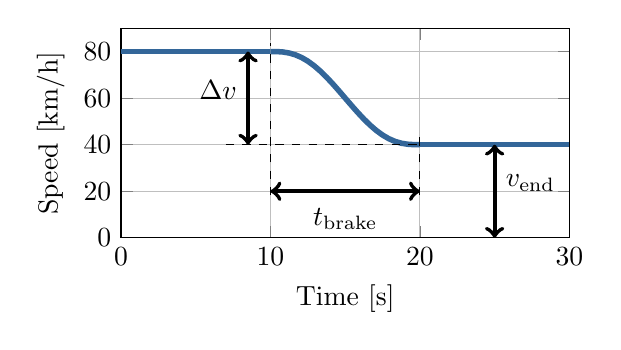
\begin{tikzpicture}
% Definition of the constants
\newcommand*{\tStartBraking}{10}  	% [s]
\newcommand*{\vReduction}{40}     	% [km/h]
\newcommand*{\vEnd}{40}				% [km/h]
\newcommand*{\tDurationBraking}{10} % [s]
\pgfmathsetmacro{\tEnd}{\tStartBraking+\tDurationBraking + 10}
\pgfmathsetmacro{\tAnnotationVEnd}{\tStartBraking+\tDurationBraking + 5}
\definecolor{mycolor1}{rgb}{0.20000,0.40000,0.60000}
\tikzstyle{my annotation}=[<->, line width=1.5pt]

\begin{axis}
% Define properties of axis
[
width=0.6*\linewidth,
height=0.35*\linewidth,
xmajorgrids,
ymajorgrids, 
xmin=0, 
xmax=\tEnd, 
ymin=0, 
ymax=90, 
xlabel={Time [s]}, 
ylabel={Speed [km/h]}
]

% Plot the velocity
\addplot[color=mycolor1, line width=2.0pt, domain=0:\tStartBraking]{\vEnd + \vReduction};
\addplot[color=mycolor1, line width=2.0pt, domain=\tStartBraking:(\tDurationBraking+\tStartBraking)]{\vEnd + \vReduction/2 - (6*\vReduction/\tDurationBraking^5) * (x - \tStartBraking - \tDurationBraking/2)^5 + (5*\vReduction/\tDurationBraking^3) * (x - \tStartBraking - \tDurationBraking/2)^3 - (15*\vReduction/(8*\tDurationBraking)) * (x - \tStartBraking - \tDurationBraking/2)};
\addplot[color=mycolor1, line width=2.0pt, domain=(\tStartBraking+\tDurationBraking):\tEnd]{\vEnd};

% Do the annotations
% Show vEnd
\draw[my annotation] (axis cs:\tAnnotationVEnd,0) -- +(0, 10*\vEnd) node[midway, right, yshift=3]{$v_{\textup{end}}$};

% Show tDurationBraking
\addplot[color=black, dashed] table[row sep=crcr]{%
	10	18.2\\
	10	83.6\\
};
\addplot [color=black, dashed] table[row sep=crcr]{%
	20	18.2\\
	20	43.6\\
};
\draw[my annotation] (axis cs:10,20) -- +(100, 0) node[midway, yshift=-10]{$t_{\textup{brake}}$};

% Show vReduction
\addplot [color=black, dashed] table[row sep=crcr]{%
	7	40\\
	20	40\\
};
\draw[my annotation](axis cs:8.5,40) -- +(0, 400) node[midway, left,yshift=3]{$\Delta v$};
\end{axis}
\end{tikzpicture}

		\vspace{-0.5em}
		\caption{Velocity profile of predecessor is modeled with three parameters: $\Delta v$, $t_{\textup{brake}}$, and $v_{\textup{end}}$.}
	\end{figure}
	\vspace{-0.5em}
	\begin{flushright}
		For more details, see \cite{deGelder2017assessment}.
	\end{flushright}
\end{frame}

\begin{frame}{Braking predecessor}{PDF estimation using Kernel Density Estimation}
	\begin{columns}
		\begin{column}{0.6\textwidth}
			PDF is estimated using Kernel Density Estimation (KDE):
			\begin{equation}
				f_h(x) = \frac{1}{nh} \sum_{i=1}^n K\left( \frac{x-x_i}{h} \right)
			\end{equation}
			\begin{itemize}
				\item Bandwidth $h$ determined with cross validation.
				\item A Gaussian kernel $K(\cdot)$ is used.
				\item $x_i$ represent parameter vectors from recorded scenarios.
			\end{itemize}
			Right figure shows marginal distributions (red lines) and histogram of data.
		\end{column}
		\begin{column}{0.3\textwidth}
			\begin{figure}
				\centering
				\vspace{-1em}
				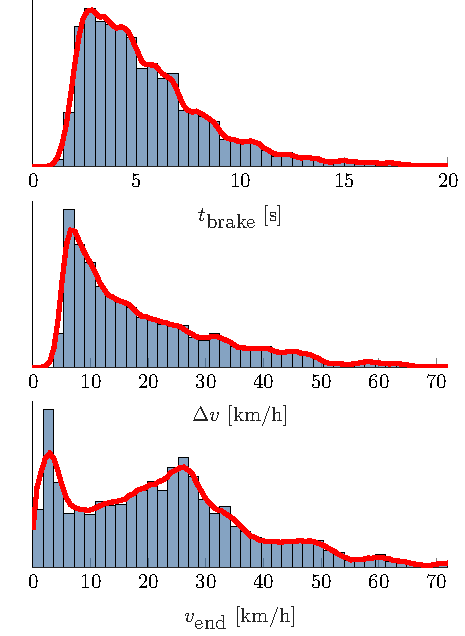
\includegraphics[width=\linewidth]{KDE_regular.pdf}
			\end{figure}
		\end{column}
	\end{columns}
\end{frame}

\begin{frame}{Braking predecessor}{Test results}
	\begin{figure}
		\centering
		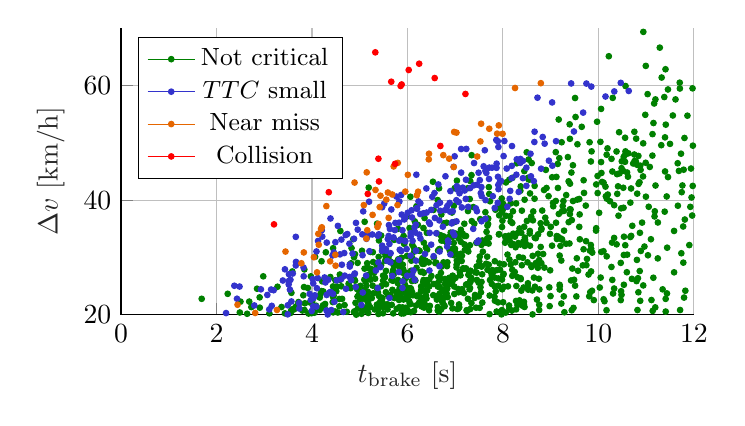
\begin{tikzpicture}

\begin{axis}[%
width=0.6\linewidth,
height=0.30\linewidth,
at={(0\linewidth,0\linewidth)},
scale only axis,
xmin=0,
xmax=12,
xlabel style={font=\color{white!15!black}},
xlabel={$t_{\textup{brake}}$ [s]},
ymin=20,
ymax=70,
ylabel style={font=\color{white!15!black}},
ylabel={$\Delta v$ [km/h]},
axis x line*=bottom,
axis y line*=left,
xmajorgrids,
ymajorgrids,
legend pos=north west
]
\addplot [color=black!50!green, draw=none, mark size=1pt, mark=*, mark options={solid, black!50!green}]
table[row sep=crcr]{%
8.32158404997322	32.4990183441476\\
8.69018477485853	29.0073161281332\\
5.7192915765925	33.0532061991575\\
7.96926055383733	20.0477439070678\\
6.27963680378662	22.9812285619239\\
5.04156864932705	21.1391131494147\\
6.98347916186596	36.1657475922906\\
8.60431942755366	28.5688500961669\\
6.31499588277288	22.3465721243166\\
6.94754342306139	26.8106144470288\\
9.18792329041439	25.2171888719362\\
5.69967267881371	27.7717415688243\\
4.81067267214372	24.7711893491549\\
10.4842314888387	23.4605013717425\\
9.4417810991641	20.7642150964074\\
7.93859782690857	27.8517551976808\\
7.19123663895397	35.8698450217266\\
10.8695827752074	34.2870446675879\\
6.76683253925445	35.9565185003456\\
6.60576646309487	25.3983923335072\\
8.88669417607032	36.9173266594838\\
7.24730355955678	20.6702156646384\\
6.3774899016157	29.4191808569557\\
5.99180708196716	20.9540376317105\\
7.86791511295173	20.541191786588\\
7.67554552163554	35.5321669368762\\
7.41736629887667	27.4196166605054\\
5.27540416805465	30.9081159604684\\
6.66163788744669	31.3656998587333\\
8.4194382588988	29.923382101173\\
5.90219636893769	27.314364865566\\
7.9894356298425	36.3940478997118\\
3.55382636721227	20.3067716052352\\
7.00642324061675	26.406601658394\\
9.00249545915566	35.3334668307202\\
4.20037101042806	29.3232146939167\\
6.78586167594864	25.3810240902838\\
6.08221732395755	29.4250399858392\\
7.93044510417625	38.6330012935525\\
6.66122207495063	20.5297066089088\\
8.66672687347409	33.4356922523257\\
9.10711775238433	48.3701638988017\\
7.72839288555361	39.7933943657306\\
6.27917839802492	27.4663014983407\\
10.8373282872961	23.9071080628703\\
8.14703461900668	37.1796581556879\\
11.1370850119417	20.6586240541769\\
8.36544840088233	32.2311380491971\\
7.34700407568075	36.3287875921954\\
8.25240419271556	33.6107983868075\\
9.18889132659392	24.3938054000464\\
10.5684368691657	59.9084178041459\\
9.28765303629356	20.4239273460326\\
7.6704491690938	30.1146805117152\\
7.1657718376999	28.101728123744\\
7.08316479694663	29.3278276740945\\
5.80230622312316	26.0554246793294\\
8.8227292498859	38.1723518126051\\
7.91625492296269	34.0022429692328\\
4.99079028064062	23.3338643271465\\
7.31511628125484	43.3269057818384\\
6.64364512778735	26.6192822052989\\
6.11288471013299	27.5311230256792\\
9.39752328738859	53.22152881416\\
7.11482572258955	30.6228575430622\\
3.65839940072381	21.3595765129636\\
7.54893750380987	28.4048226264434\\
9.74122584450742	32.8264468450706\\
11.4056009072	62.8380534297078\\
5.40390519454819	21.8958693452976\\
9.59935067872135	35.3256883223094\\
10.4115711503865	42.4066884859692\\
10.7846302287497	46.7329716109823\\
6.98955171339008	42.0767998602439\\
6.1335335123672	31.7142966479692\\
9.32228422671208	32.3782870977361\\
10.0563866938344	55.918108818135\\
7.18671217940085	27.9961677052972\\
10.7909368135678	50.7279841061752\\
7.3233454251679	26.0527247840623\\
5.4486483928623	28.6459373484522\\
7.11902611938908	34.8185292519768\\
6.63557193227166	21.3265143525763\\
10.6191072216781	44.0805973702018\\
4.94577694260574	24.814074669743\\
6.68093014293542	23.7237970470304\\
5.91952358080449	33.7399707064951\\
5.64219872494581	23.4399483136907\\
3.69035978549693	21.5581622376294\\
7.41523057163695	23.432447967575\\
6.65387201515708	23.3492094615402\\
5.90887864554808	20.7335192839063\\
2.97912679571778	26.6901396988471\\
8.71230957006057	22.6340504509179\\
7.90289899219565	26.3285246377764\\
9.80766375463803	23.20260588136\\
10.8609785522372	43.1205609545508\\
8.12785180908783	21.5937064885935\\
10.557828984711	46.6793582540553\\
7.49444557514275	23.191504511178\\
6.69797855821503	33.8533623396489\\
5.4892956277003	25.913240772799\\
9.41683833130479	38.3560155902977\\
10.7982711065137	25.8554753695368\\
5.45684843450454	22.1785583986189\\
5.32234623158164	26.2781849927643\\
7.34008048649538	22.0225425322114\\
4.90314365252166	25.9359804636783\\
4.86488874183451	33.1771970601578\\
7.4001821584353	35.8724652552385\\
5.99008991957187	30.2412278349648\\
4.04714392206324	20.6572111769716\\
3.59758889631095	20.96114183872\\
8.13664883757941	32.9668220635142\\
5.25285135037963	22.9029121063681\\
5.86139562449765	33.145773824255\\
11.4301831547335	40.6298838151594\\
10.935037007809	44.1306912318259\\
6.18838517810933	38.9230825599569\\
11.8210684825632	24.1745645184986\\
9.28105980524167	34.6683131564915\\
3.83305897604124	24.8177211286598\\
7.82437218549369	23.1303829540269\\
5.70814242632895	26.9244703582781\\
7.56812359976156	22.1084543871074\\
10.1272556839296	22.346887155953\\
4.47973722544707	24.6564506297384\\
6.68511076823537	26.3506976967714\\
11.1945758999245	57.5766172785707\\
4.5715365068157	22.7436743775799\\
4.54109988927661	20.3744706820089\\
6.63751815895568	24.8987442222679\\
5.99106270146536	20.5238360102252\\
6.36651599094815	21.7673525905759\\
5.9496680551296	25.1824430778293\\
10.8090893369742	46.1620644469642\\
5.38127571714945	23.9123653875733\\
6.96917834736881	30.396472829227\\
8.12184333543321	33.7771439956244\\
10.1700675511841	20.7726130824544\\
5.55243290241952	25.3084260748391\\
8.62081922184519	20.0469479882826\\
10.1483695641252	42.3459380732028\\
7.6768252681272	27.8227395405411\\
4.767441319072	25.4080167360681\\
7.22657294271828	28.0753696868193\\
7.2664283079441	22.7725977062406\\
5.40294662221397	23.2593839712889\\
8.36675578337194	22.2520348010406\\
8.45762780433402	31.986769142951\\
10.2999187105636	57.8407326309383\\
10.3294245663698	33.3947174327465\\
4.58329200241107	27.0029575868149\\
9.4053000101545	42.8622255362344\\
6.82014762116963	23.7080034067942\\
9.16847091564552	54.0635863425669\\
10.3901060537999	44.5254171651725\\
5.30003949397006	27.2993762984424\\
7.02762987389044	28.2432875500122\\
10.3071581203408	23.6948722728603\\
11.5855858472012	27.3914226553614\\
6.96987016035945	32.512250904827\\
10.8379113389597	47.7082571058977\\
9.95435578133343	42.7322504135002\\
5.47724923335724	21.4478926202296\\
7.97900526920803	20.7927795095407\\
10.1728442413161	47.9140974906151\\
8.44518353747411	35.3315450497527\\
11.9393535209049	45.5082677573107\\
4.00814108591965	22.4392408308418\\
4.59948321615013	26.5864728635615\\
3.71728038125613	22.2017607954158\\
5.54864544362768	21.5184711474089\\
10.806926085945	29.560029221816\\
8.73541879647646	30.631288582163\\
5.99910009427072	37.1760423326216\\
5.1738135997447	23.8485170995276\\
6.06663665109402	21.8507191071246\\
10.562542970653	32.1192161803257\\
6.38665726754033	23.3851113262326\\
6.9409416992427	33.8863817700842\\
4.44220052255129	31.6025220458977\\
11.076339927272	45.7856732015513\\
6.34311955748178	27.3007113218762\\
10.4209929264004	37.2770879182748\\
11.9790836494677	49.4999630741609\\
6.97967957471196	24.9123053837804\\
10.6691138460489	33.5547677667218\\
7.84245628613005	38.3187355614938\\
1.68992120357191	22.7662243479975\\
6.8330630190547	24.5320241892114\\
6.33774346486448	26.0570158166733\\
7.6246997087236	32.5620089248818\\
6.71060214912827	32.939059773688\\
4.89108664661679	20.577129733041\\
10.8416669846137	42.8273920494461\\
5.10731315169309	21.1969329748124\\
5.94219997650438	26.1962044624358\\
6.09167814001786	34.3360724123769\\
8.50175151574931	36.3563964084139\\
10.0562206034859	46.637368415544\\
9.87092570555433	30.8334741692555\\
9.79350074766234	27.0059652529562\\
11.0378644980321	30.3681669094071\\
7.40823137237338	22.9161324268831\\
7.53016983290435	24.7854263727564\\
6.31154438332767	29.8466256499069\\
6.64097224158644	31.1875787214033\\
10.3820245681182	32.2726071699157\\
8.73652145356621	34.0230709493553\\
5.96265918256527	26.4478343285368\\
6.67074144983895	24.8651441597416\\
8.31749603607712	34.2967808757936\\
7.67247074454587	33.3340355444709\\
10.5626956160419	47.9646829118533\\
7.06487155022817	24.4644742678255\\
8.20692280291141	32.3601331762641\\
8.09606330092999	30.4842261368771\\
6.80935499290505	23.8444920995552\\
10.5356688839085	33.6079514088572\\
11.1814254143834	38.0412837923758\\
9.15201416309456	42.1191925168552\\
9.81534660948749	50.0954885452602\\
6.07498644655937	27.6635546443233\\
10.4759665517934	38.5659486347164\\
5.92339168746716	20.2212766931451\\
7.03588589043733	43.3951853516331\\
10.521349807209	42.1491319688976\\
7.03401637349894	29.4637374429326\\
7.23918510265267	20.7709319873532\\
9.12034467416808	44.044207581766\\
9.82296145050226	31.1602628376824\\
6.0443450842061	35.1231511699984\\
5.82127023743441	28.4303301790783\\
8.76400698005394	24.4044148083608\\
6.39892822254642	22.809141882514\\
7.89774294979785	22.14008646966\\
10.1965224355715	40.9673190275032\\
5.27184373653597	25.060145145482\\
8.27588930151427	20.9219707686091\\
5.59743106407765	21.5524409463078\\
7.52369663105729	36.6751303479963\\
3.92822829795355	20.1920271785854\\
4.48310669507298	20.5598435734508\\
10.9643244376695	31.8859032552853\\
8.06215057274974	37.2562175505993\\
8.16260974631911	39.4200113181455\\
7.34496673829018	47.839186086647\\
11.7790171260749	29.0808127034685\\
11.7113279741559	20.8078846147139\\
8.56728933601402	32.0303019263465\\
5.80705694106609	29.659710217627\\
6.13758448250824	20.6492482754426\\
6.94203690955979	21.1006236178801\\
10.5297875200694	47.541461425599\\
8.39651586162857	28.6310968766739\\
10.3950263245185	41.0873094680677\\
4.88319859728213	26.1530327154226\\
2.64181117521385	20.1547540375772\\
6.1144781038924	23.3896119741275\\
8.33738803520874	30.0486448915779\\
5.84170641579351	29.1086074146515\\
10.4683857178895	22.5392178542785\\
7.86869642748035	27.7713915435023\\
9.36043571485327	47.5043118528398\\
9.60725780748327	37.4960505974391\\
7.1832743074765	23.7660592839446\\
6.02098144583266	24.6084368889195\\
6.82753762053879	28.4685054408021\\
7.07070301140875	23.9007007935567\\
6.99507724521685	31.5081429528362\\
5.9631913534687	21.1919935636931\\
5.28608710915146	23.7231167035655\\
10.8833821839132	45.2646765495252\\
5.38648544871103	20.9840151761637\\
7.30879295913863	32.1235731354027\\
3.91372155961543	24.6492226971981\\
11.1111694727881	22.5541701801521\\
5.52214064363783	26.6106833577469\\
8.17363366873702	32.1617105135162\\
10.6843355191643	42.0283364156019\\
5.92874948098215	32.3648426193816\\
6.41426482434232	24.214662953355\\
8.0086763224693	39.3143144438668\\
10.2861923166097	32.5814225313821\\
8.14618827516544	33.5260053124621\\
4.45292890631975	23.3350343892141\\
11.4579038215492	44.0118144237274\\
8.91166053599559	36.0206646587465\\
4.59482860115972	34.6078656274429\\
10.7009129133346	26.2500482772956\\
11.7369656627391	30.7172214853528\\
11.5852428602004	34.6135482559619\\
5.10713037661835	22.9008684715123\\
4.911465852831	22.0629472257845\\
7.68969457815536	35.8230592489\\
5.83040502099001	21.2947944624293\\
11.4092131934711	22.7548322820037\\
8.29123093125287	46.422886532995\\
8.27460021344563	22.389164266693\\
8.59775530321583	28.3323080845212\\
11.3248454557373	61.3934715421603\\
8.19531176970378	36.0009537343838\\
7.31842072524749	25.6811728459397\\
10.6865541009575	33.7513084844882\\
9.98293226043886	44.2080919114589\\
11.3453406395677	24.4165543279713\\
11.1333963897857	51.5124692159659\\
5.09609015143536	26.1090477120594\\
9.76067911436531	29.7245255145466\\
8.56776152929833	41.1619297575085\\
8.63471263446797	38.0192489943334\\
5.07762707448429	20.7630471225586\\
7.43725976741274	21.2162633531095\\
10.3303665164997	39.1060891919832\\
2.50233760570892	22.2756645871128\\
7.26834688076734	38.0790200744806\\
7.99772526044609	38.3251746786756\\
9.24003641633066	33.1100773548489\\
5.18012851875254	21.9168197398706\\
8.26562691915708	31.7661271919718\\
11.3169036638574	49.583946111349\\
6.77109554829068	22.9612458204485\\
7.20184116893962	31.2787205331101\\
6.98682167556184	33.8702259053034\\
6.46942132954323	21.5389665825858\\
2.72959010009663	21.3233221332937\\
5.1839055627862	21.2842296652694\\
10.9146007557807	36.0664380634287\\
5.53930649743681	30.2147245024423\\
5.13525854602915	22.581179895141\\
8.30384730021122	21.680658314368\\
10.6009094418439	44.8191498141557\\
6.98197337579341	23.6055605374892\\
9.68956615124974	31.4167532994458\\
5.98616679803335	26.7700384541634\\
6.63445194914669	20.7157738116548\\
7.98366293383012	24.4271990688812\\
5.46295743449256	22.3831678353079\\
11.5593099356659	54.7681407207474\\
3.73398806797533	22.0137310279465\\
3.56933574297038	23.8080048714523\\
9.95040494473612	34.6695582052466\\
6.32981946708113	25.704864528845\\
7.00685021111412	30.8302705969052\\
11.1681267291523	56.8616077773225\\
6.24486386846987	22.1180268835205\\
6.55179805202067	29.9774086548365\\
4.57312483089162	21.4582349245228\\
7.10114680005244	26.9196260256143\\
7.27559572126061	26.9449445026623\\
10.8889545269742	31.1237410550149\\
6.29721180078953	21.4342756942245\\
5.12217446420323	22.7679111011382\\
10.2733605739182	28.3254417405485\\
6.2866110548739	24.9403180109857\\
5.37706878114423	21.4793670089827\\
5.45340008071687	25.0073927186584\\
7.83053847752964	29.3221971605133\\
8.53763763465144	47.0860645286847\\
9.90391705164221	22.5378237847444\\
10.2744045755121	47.1975487173294\\
6.06906001502984	20.4332217528927\\
7.55628096774604	28.4263964048043\\
6.53351509743162	43.2002751299477\\
11.0306516764892	58.4973248084747\\
7.14461265305466	24.4539179177079\\
8.75930460854173	20.8087023737129\\
7.06738043455999	21.0634042794006\\
8.38413810181411	34.2989070045323\\
5.7008234605646	20.2200947653524\\
8.16137687007128	36.2584610493209\\
10.1085068526271	43.0276981860312\\
6.50177617642749	26.761194219929\\
5.68399591669316	24.3352912344557\\
7.18807125159818	33.7406064525999\\
5.39709030078204	30.0801405321041\\
6.66849609049699	25.9175469404795\\
7.71285253786293	41.0681414901418\\
6.45286213493814	20.7572414323836\\
10.5591993386893	50.87947429542\\
3.95742223759669	22.1333945800356\\
8.56029524405514	34.1681294883538\\
8.59055955272455	36.772900702471\\
6.06108686883471	24.6272187352692\\
10.5675111812995	48.5050405541064\\
11.3962839267413	45.0001598859619\\
8.42632487731562	32.7303700050333\\
6.15365967155054	36.2814789026044\\
5.18888078469557	42.1762525168485\\
4.61868270020879	26.5819784561102\\
9.53817122519163	23.1825739769875\\
6.61624558607046	34.199709633797\\
7.02740372246337	33.8560681603412\\
7.15343533575566	34.0269660278581\\
8.28148110387613	25.001617383951\\
8.61514220151363	24.232345986578\\
11.1507781636971	26.444467470288\\
7.76732344646994	25.3554601420254\\
8.34654116402383	22.5025206631393\\
3.97632044630519	26.6882316496398\\
10.1764817027858	40.2444581819869\\
7.78189761488438	27.1832284580032\\
8.80477421448449	28.9917432779499\\
5.0079530668033	22.6131100623764\\
6.87879797568323	25.312596984934\\
5.54876191839184	23.9256234795093\\
7.5125681553861	21.1872063233696\\
10.3799343285228	48.4819120955422\\
7.31117593555455	24.6679515154196\\
8.49810920434651	48.3465263465957\\
6.23537897701763	31.2258115013202\\
10.290938727354	26.0660477361204\\
5.4895127480501	26.8156554500181\\
5.58297235043943	20.9175687539103\\
9.18113726159808	47.3243564173341\\
10.5324812390636	30.419019777071\\
5.7134202142105	28.5664686648614\\
10.8285169042858	26.3628206862421\\
7.27459869998652	31.0236681010574\\
6.10139687083967	32.192829811609\\
11.7452255771298	41.3801861251666\\
7.26452191589296	42.0742323868798\\
11.3887761557815	37.982055649954\\
9.49116561009471	26.0890102089316\\
5.7037463772916	27.5262075321625\\
6.78542879333091	26.2318060232941\\
5.20861288444894	28.0578767291422\\
7.50519956511464	29.3000015761123\\
7.29274343213879	27.402760873374\\
7.97505830901365	40.2775958594314\\
4.80949886863299	24.6251731950876\\
6.75497305199611	29.1375802035891\\
6.14201695845588	30.9985758892031\\
8.04307322798735	38.7857280491311\\
6.07499629937281	24.4976514482831\\
4.92703382804185	20.0000232857693\\
10.7571860976856	46.8190906283383\\
9.25272081964223	38.9708946040191\\
6.20129844796728	23.2054077591967\\
7.9300395373962	28.9097273714338\\
6.70383922378976	20.8963474033885\\
4.08415499401297	21.5665350468041\\
5.10099477160641	28.029137963777\\
5.4494974981692	33.8108619505248\\
4.59124013471061	26.0872508767505\\
8.45891026880819	33.4515977916611\\
9.40269028682132	37.5649879514769\\
5.82919422764778	29.2154310898643\\
11.4358141334297	23.7092432052947\\
5.20283206393242	26.5783450924675\\
10.0593529321214	30.95088182743\\
10.9817185632946	54.884451709752\\
7.77867710891983	27.7747174392785\\
4.6139231509557	24.9528279810372\\
7.56763241256324	32.9508028687149\\
7.0700283916365	33.3445807528274\\
10.8778188859559	46.0046159930996\\
7.76889784770063	26.7947941647356\\
5.22263777891243	30.9492376767259\\
10.4421843829713	44.6638248251441\\
4.82878610418849	31.6152905710413\\
5.0367852651898	20.1546147546402\\
8.80664531871482	35.0500034637487\\
5.91675110338699	22.6390751626082\\
5.21556714973057	22.8242903685713\\
6.3354922106827	35.1271256777763\\
4.90230149515401	30.5669102548862\\
7.7295354742095	26.0469789123437\\
9.19142731368759	24.9676782318575\\
11.685817242341	45.0925970724781\\
10.0287649764228	24.7370332726903\\
6.45813482133286	24.9504199739492\\
10.9392606965799	25.1047558743056\\
8.13391404903712	43.5700070766643\\
8.2764336259645	39.4209274849085\\
5.50307446764384	21.2847022793847\\
7.31555310483966	20.9873954294763\\
8.10612859053873	24.939660900493\\
7.34162658620991	44.3596943197468\\
5.07160185215983	22.8330301662929\\
5.90191483521533	28.7268801752169\\
7.55116949677956	25.7198008987927\\
8.62325631074424	30.2625435722596\\
5.57373131454595	21.5139342460033\\
3.62468661314671	20.9112628919322\\
3.84358303580571	20.8087750367795\\
9.82864994112473	23.9285495285307\\
9.23000069991261	50.0947285278895\\
9.51166139283928	25.0578992430191\\
6.6304126871503	23.292382656646\\
2.90624034925275	21.2203668652913\\
9.37758542505797	36.1486975175468\\
3.85130792493688	21.9857105948105\\
9.13061422694092	33.2097347871102\\
2.84917988435961	24.5268756163452\\
10.595695949017	27.4076426262751\\
6.76371927483449	21.70134790049\\
3.84034798624938	27.8979361799875\\
5.24949596304284	27.9278645224715\\
5.8974047120781	21.2722419475511\\
11.7757936746255	35.391844694182\\
7.45428832989063	26.060629598172\\
8.55886965329059	43.5785480505001\\
5.28163526435827	29.1799331003535\\
9.52126324774798	54.5060390857044\\
3.58789613177299	27.5404582256975\\
2.90370620420772	23.0198270567858\\
6.87435584726408	26.4340163533445\\
8.86814477861502	28.2068963390644\\
7.70350706078346	28.7197634400255\\
10.9905727222356	46.513451051395\\
5.59633033410448	23.2714002850944\\
2.23461753572585	23.6374774765584\\
10.4335718932989	51.8454503461662\\
6.92789361779867	31.4329497909957\\
8.21578176677866	34.1360850960182\\
8.19927424586322	43.889462321539\\
5.35733455510253	24.6679040219659\\
4.98993775630608	24.1269335038268\\
5.15667238881435	28.9769749805948\\
5.42832616787746	22.2537489652863\\
5.6492810736014	29.2438949682857\\
9.20459062997367	31.9988065000592\\
5.13280591254752	21.1857964081297\\
5.45945185546691	21.5232564562871\\
6.08228915554226	27.4851792364037\\
6.45852809171462	26.1307858395097\\
8.02035859607405	28.7950023704884\\
5.97799702739441	26.5356671621368\\
8.89917393344673	45.2711369880536\\
6.18975324023709	28.1844798097092\\
7.33434596823165	26.442572303155\\
8.79122137005374	31.8202316602218\\
5.48917064376981	20.2414063659479\\
9.86660855839903	24.1709229972781\\
7.14195281179722	30.2911330042584\\
9.55604309702355	40.0793325489084\\
5.83514247724438	24.634385581368\\
4.05274787474046	20.3451303024007\\
6.10087080925548	29.9188427869243\\
9.10750727581441	39.8390275369358\\
6.44794402747445	29.1235390245717\\
6.7793675426646	21.4750613614448\\
7.70952959684258	33.4355822138582\\
6.80704075342585	24.5948534623378\\
5.52160022443791	26.6076885212643\\
9.84154224794242	32.1584874911288\\
11.9639977713887	37.3035022547149\\
6.82037894324438	32.6321804903936\\
7.15524491577599	34.1581166243875\\
4.3844182576513	26.5745406711622\\
6.90518835721459	34.3214000587913\\
5.39316413890605	20.1179989763513\\
9.4025801344194	50.6920929662203\\
10.2182582444348	65.1113161887287\\
9.47819256168326	21.1810408732896\\
5.40277067162968	32.9550539209245\\
8.4392261335251	21.8240138815947\\
8.51841170699392	25.0136121561008\\
8.51548253576108	29.1343844238266\\
8.44095268090704	22.2432615776249\\
6.02615619017841	27.1536733938126\\
8.19600332947772	27.8381822568883\\
7.92194482553498	37.3373926488384\\
10.6026818436613	30.4754397550872\\
7.69193736315632	36.7858943990197\\
10.2430910302651	39.7988456439549\\
9.05008096453591	39.5110671375222\\
9.84653182709156	27.5528807005821\\
9.57277175342577	27.6600378396201\\
8.76054066715446	21.7417783854683\\
11.1760080446904	37.1476150015389\\
10.077590070594	43.1667016156737\\
7.09753839429662	27.4425017086669\\
9.1122751688263	36.0442050908713\\
11.8028101870105	50.8430307145318\\
11.7035974253143	60.4986609506429\\
11.786286561932	45.3015609202772\\
9.67296565428887	28.601347267001\\
5.97535225367858	24.0027879261731\\
8.52928405664238	24.3607714662953\\
5.47020967251226	22.7729514337518\\
3.43371121702348	20.2245831203646\\
7.26225444422066	31.7381281563119\\
7.98076236535966	35.3051092196239\\
9.22247002685878	29.4444329967987\\
11.2440825261444	29.822731950124\\
4.44103368638374	24.926703526568\\
6.09759972609452	23.944692559023\\
9.84215545182114	46.7416288260101\\
11.7064955098289	59.4762310563291\\
5.53980453882073	21.7520013891724\\
4.52793928947768	24.9025079250946\\
7.32086317748109	25.9005564705891\\
5.87822548540507	29.9349016679657\\
9.27465298443489	23.1880541432946\\
9.8479414858904	31.5051778639811\\
9.45303373932657	28.0489405890622\\
5.36726681579596	24.5759621893931\\
8.06319374704593	43.0772438141941\\
6.35830928543975	36.8626069679023\\
3.56620380106373	20.7729966821781\\
8.25941629850976	29.1449867845018\\
5.04758858352259	31.152647375572\\
4.44346116655426	20.3911816872497\\
10.6275862962097	48.161071241817\\
8.53488742366672	43.6326122590081\\
6.84389543276916	23.0663619850159\\
9.44325530875272	36.504889705249\\
7.72148583514449	23.3338249756194\\
9.95339871677041	35.0931013177232\\
5.59528143099706	21.7379687726561\\
10.7518274248931	47.9541768601681\\
7.84962507876633	24.0688478344004\\
5.22628965410714	26.1051234862894\\
8.36874566585883	26.3667893440962\\
5.01628057373024	25.033792187359\\
10.0155777987108	37.780071332899\\
5.16706512244904	23.3359901631568\\
10.4750226758834	24.0916853811133\\
5.86700660191545	23.6369973848708\\
4.15123910672662	21.0393506492506\\
11.8101991906341	36.6037183882569\\
6.55232581579152	25.3509708509043\\
10.8182803765073	20.8053875242729\\
10.9383024811655	49.9072328624958\\
10.191082232951	49.0288799895703\\
7.70004312099445	32.4152331106223\\
5.87265560796448	20.209825116859\\
7.97530186520734	37.9082462436291\\
7.82474259511628	26.4704068913213\\
4.16305142016481	22.9840402350006\\
5.87549096454617	22.881863399438\\
10.8657504495907	27.6129109882743\\
7.01299050112803	34.1517748513571\\
11.4998695683504	49.812203678493\\
8.64978996485458	26.4675754777173\\
7.91958113317156	34.0611686122365\\
5.91276534353231	27.8962214256906\\
8.75866616417075	29.5421573034847\\
8.80398620481166	34.8443983863901\\
7.3011788526412	24.4092540849096\\
8.74640726318394	29.2709948071063\\
7.65691719599328	34.4523091758467\\
6.58406894202822	29.0066801032071\\
8.43294918772891	24.7406388275036\\
7.06792695760174	34.0499129068139\\
4.63117989261324	22.7583837540906\\
11.7938970295147	22.9821589836291\\
5.82499566741297	23.3836881730964\\
6.71361587887045	28.390477508218\\
9.85715017001789	48.5015174489545\\
8.98918320722587	27.7422097042844\\
6.40687010709936	34.2789969530282\\
11.6151927562927	57.5747402462458\\
9.7481051601856	28.643398264429\\
9.51164170060297	57.8187449061313\\
8.60342954948932	46.4620114106641\\
8.68781784803435	33.3427171544817\\
8.05843317467416	20.3626583671577\\
7.04509493270181	20.9853747453668\\
6.93259884819891	37.8301696631697\\
10.0633094362796	44.7297859520218\\
7.07516730804144	30.361050730708\\
7.56480142907096	27.0458138731288\\
5.57339684501928	21.792832462085\\
6.8210486010599	36.0482716191684\\
4.88080943452442	30.0140533914446\\
4.23059623940858	21.6254861255465\\
4.81731693305633	28.9652200879423\\
6.34252865493178	32.5661837395916\\
7.8317080925496	22.4313555354717\\
5.36392083223915	35.8822053476491\\
6.9723078423242	38.9951416758692\\
8.02102909484986	24.8594588426065\\
5.47890701324641	31.6096448425189\\
11.864795362632	54.7338572227065\\
7.25485254446189	25.3446015231072\\
5.35841029107193	28.5351030538516\\
8.24798519395409	27.44394387954\\
5.20647743409065	21.3315958787897\\
4.95332980711414	23.1640592045122\\
9.69031461175637	43.4609751912202\\
6.28844088685017	24.3168570277976\\
9.43451306569665	44.8059175975246\\
8.13548386476967	29.6246247304523\\
8.95592103025885	40.6812490121996\\
4.26054783267196	21.3017274240878\\
6.72811798349435	22.294981732697\\
6.88408301544672	31.2285244596194\\
5.76304976784199	23.9216110349402\\
8.99702483938824	23.2414337266331\\
6.80147536633176	23.1990065324568\\
7.75419148135168	27.305905892309\\
9.56062415381	49.7478742477751\\
6.38601752046515	29.3580980057584\\
10.6692923370993	39.5552590367349\\
5.73010089735138	29.0338822975368\\
11.9510406021679	40.4591461733191\\
10.4847379004886	45.5706673775937\\
7.64878450530544	28.8927546370199\\
4.95613573258589	29.0366611587183\\
10.7531055816046	51.9238204167331\\
9.39382721913277	32.4269190805964\\
5.35881572545395	21.7398578631468\\
4.94510438910878	24.4562149441411\\
6.18120570601801	21.6020632977492\\
11.1961261807079	42.5403188736382\\
8.59207848577151	37.1088334406\\
5.61171907475781	30.2579382533508\\
9.65091963221776	52.7858173813345\\
5.10376197059967	36.2112797541452\\
11.9038993151823	32.1425953082067\\
8.20984545195319	38.0461532026725\\
4.97950481778819	23.438124176808\\
8.00640840208754	26.9543681057838\\
7.31987224740887	27.6726402776233\\
7.02958615728074	28.7226125948183\\
7.19316377170365	32.2644746269363\\
5.46878415423751	22.9445579850838\\
7.44967912810517	28.4125931619528\\
4.06607093788544	30.1012935023217\\
4.44004023998575	23.1273388104817\\
7.53956309966743	23.8841521381302\\
4.73041945932947	20.506856855068\\
7.1355829720565	29.3651433797887\\
6.36520987596836	24.2230545437524\\
8.52388890086142	25.4843369492887\\
11.759697745185	42.5534189161619\\
10.9409149191662	69.3614895600771\\
6.32534088451649	29.7012006596995\\
10.4895243020147	46.7745780513118\\
8.04528054556941	32.5584263296105\\
7.07999396600724	21.787758570938\\
6.3883095832634	31.7176926508326\\
5.06750441058773	23.193586335612\\
5.89622550017041	24.3686994163062\\
2.68559070392777	22.2806218304134\\
6.8677487125712	33.5614572752752\\
4.62544901644731	26.4945890675364\\
7.71877380726652	20.0917756411216\\
8.30712980700658	26.5322657469564\\
8.34749322027807	35.0418827455506\\
8.13251898022199	21.0578321181598\\
6.34602828595149	21.2305213090596\\
4.88003322621203	20.4575692460403\\
8.16413141173624	28.745810470053\\
7.22654100892883	33.732081151106\\
9.239287711076	38.0601232082756\\
7.63276491886491	37.8852039712918\\
8.36530076876839	41.6346578723838\\
6.2858702456184	29.3084230015595\\
5.17879073810412	20.3048093732537\\
7.30525805849797	40.1834707906626\\
5.19582968853084	27.0094596505711\\
11.1907297121927	21.2683317442918\\
8.4727009650447	32.5477546072657\\
3.3618133215223	21.3365082748232\\
7.70513076467245	42.2616945454805\\
6.53968685039668	23.4033478535798\\
4.96071553425558	21.0579163669939\\
5.66413733187495	26.0354726823911\\
5.21942957418659	21.2989779177073\\
6.41239257470041	31.3527809526913\\
5.98850276035384	23.5488088264566\\
10.8125582511997	41.1228034280398\\
6.70135169300097	22.7419086709433\\
6.61549308306252	22.6323081110304\\
6.00714192339046	27.0973010322961\\
4.2140060093452	25.8140160393465\\
6.31073833827119	27.4881965548457\\
10.1557888421696	40.6693716601396\\
11.2456261379604	36.0894001589697\\
5.10518034065484	24.3219660195969\\
11.0538023244252	38.83202906483\\
7.57923697820568	30.9910494792431\\
8.44785160637542	45.0586472493114\\
2.4883177834194	20.3795540312782\\
4.1643044695954	20.8267055845027\\
6.20040773375442	23.3550568715168\\
5.68451997766773	27.184618404504\\
7.09673524820287	30.4963493286099\\
5.73022499810551	22.8899151078677\\
10.5333452588434	25.2163406959829\\
10.109612017652	22.6847462141768\\
6.91499687281759	22.0433021041722\\
5.82320943102294	22.562460812202\\
6.94601258139787	33.5754004253124\\
9.22366749173541	21.9371076916694\\
6.04767580439904	21.9020167356291\\
11.6607691945988	46.4298011238054\\
9.20838542162819	33.3110171243902\\
9.61097932217381	33.1533343631962\\
3.81827076283977	23.3831657444871\\
7.22895456778196	25.2493660273583\\
3.99410394914795	20.2591975870733\\
8.0470968579594	33.683650966667\\
11.411347980816	53.1680308977388\\
8.97876847340079	21.4898632120355\\
6.1488377559851	26.1734980588354\\
6.09461275266233	25.8660194992742\\
5.31365274796989	20.9091312991484\\
6.16622771759859	25.9464572760305\\
6.94091262752948	25.7834884302733\\
8.7532299820043	26.2678183014146\\
7.11794818547412	32.7134708325828\\
4.68285017163109	21.6731896857247\\
6.40298961458373	26.0075664698973\\
9.46767715582286	39.8358870801119\\
6.00970947226385	23.0932221571528\\
9.0291931564866	32.0423922134854\\
9.69879187621178	41.2515021014285\\
9.54771084281229	29.8419407924406\\
8.66963923041357	24.8768195873517\\
11.4098973878042	20.540354385318\\
11.1002377964647	33.1671783084097\\
10.3298385321594	24.5601512244011\\
7.54963507259806	32.174686109695\\
6.74964611007557	32.9332440845915\\
7.97982472865294	26.1192692738972\\
6.31221723550367	28.8717649566917\\
8.56375700117292	34.6086472787387\\
8.45232893577263	21.3419503033965\\
8.66257928307694	40.2371473827664\\
5.67084057850098	21.7112494545237\\
9.14778773251284	46.3115907959343\\
11.9717653032838	59.5082640263629\\
6.40616141441279	25.6226057043962\\
5.90453386087877	27.4019923445256\\
5.77578780762083	21.0268349583682\\
9.37616592981011	43.2748717902379\\
10.4681342721367	29.0372160751575\\
11.9756568728177	42.4731173222848\\
6.83757803621461	29.1403498832508\\
8.37390625208486	26.2041674982193\\
11.6647633389404	39.0134555471324\\
6.92288785233505	26.1091067904543\\
9.0308472329	43.9915254629818\\
9.23001317841717	33.1881754894186\\
4.27538889577965	21.863718216686\\
7.48995199575832	25.5914380877449\\
5.12297154578358	25.7524755901004\\
5.99552317621386	27.2437579920112\\
4.17191954513889	23.4828885234778\\
6.76099195789103	33.6501955916976\\
10.9928027639306	63.4247189473201\\
9.32514126657133	40.8756687205524\\
8.05688884870127	33.4924372466966\\
5.79736927328852	25.5025953789279\\
8.38441397159073	24.1904771905996\\
8.9854628188994	34.1057678069827\\
5.52483761838619	26.4854458168368\\
8.91281348746269	42.1097093309372\\
9.18845320801121	30.3120886034815\\
5.69466420751722	25.9123158421081\\
8.19645847494556	26.7780381772583\\
9.73579397315962	39.0351237889725\\
9.12666272724344	33.7127382431342\\
5.80163301083385	34.9759429888328\\
8.4112717065569	21.556454029181\\
10.526566340306	38.659812731424\\
7.44923280733354	27.3277549229541\\
7.44337064858222	32.5331591034586\\
10.9946284769992	40.5909435794809\\
11.7302453527369	48.0977668865882\\
8.45424637695255	40.0634737723428\\
10.0473492826256	26.4738761135532\\
9.27815316840743	38.1124340704972\\
6.85028829218165	26.1249246500995\\
9.59867742246082	40.18709525618\\
8.18171423635609	32.2455375896386\\
8.52461697612251	43.8887032608876\\
7.1106387464971	26.8644763112674\\
10.2921035826316	44.9872951932871\\
3.79897686756807	20.723955574288\\
11.9253579427266	38.8207097768602\\
10.0417839810264	50.1652366324167\\
6.28336870735297	24.011793609626\\
5.55134389583301	27.6362517262839\\
6.73422776511728	22.1674483138021\\
9.46606113617269	46.0774199465295\\
7.96919930331069	39.315119234708\\
3.10774813257008	20.2233385740914\\
4.23584148387487	24.0608754842761\\
4.19615806110112	24.1170674395123\\
5.61789033778615	29.4017914888376\\
8.86106190751607	41.758690360215\\
6.71017659781255	37.4853850701951\\
8.46328126047694	33.0760502537928\\
11.1309189874929	47.7639720281573\\
6.25493109742031	31.1326907004735\\
8.39687975623975	38.1553857792545\\
9.05406032057582	38.9189950852132\\
5.14022257825938	25.0824047276776\\
6.21834750914235	35.6700885485686\\
6.80551439058784	23.4432169310443\\
8.73187166428218	28.1732583602355\\
11.1531981660809	53.4520543844176\\
10.5161406718882	45.1138855506434\\
8.01456318532721	27.1213394330522\\
7.51488184095496	30.1398739662098\\
8.78939517274347	35.9576409151864\\
9.26709667484226	39.8284111410124\\
6.67416235057333	31.4554911432839\\
9.1515727562523	33.6410963258269\\
9.17093130400808	37.5838708674325\\
10.7094562781357	35.5103887525576\\
7.82761743462548	24.9446583542242\\
8.60287444299571	28.4521356135132\\
8.62842258490647	36.4612338200929\\
6.73862172531176	24.3566597123234\\
6.3822095115281	25.2133166381151\\
6.06128441179074	40.5797788261662\\
11.3803744353462	57.9834011113157\\
8.97097030827046	24.7680205802526\\
6.34508427738583	28.8695127439251\\
4.48934623520426	26.0044793327533\\
9.97243099567033	53.6730932658932\\
6.63378886959008	40.007518402243\\
11.2859006140952	66.6114158060865\\
10.7284287739254	46.3855778430485\\
4.50967196773032	24.0930479201177\\
6.95646332481983	26.1765004391785\\
10.1739938487461	30.1758240453327\\
10.1063731015902	31.0718495451266\\
7.90453859343042	25.0519060207811\\
10.8756428721881	22.4152242681589\\
11.4401786665149	31.6886490501015\\
11.4568406565795	59.3079062163143\\
5.16665998825452	24.0207567139018\\
8.00403097520429	22.1714372612535\\
9.98408430092724	41.2237223780611\\
6.60336861119222	29.0695544209846\\
5.91997505585164	22.7222347807753\\
8.66381430512963	42.4789239693032\\
6.70109531378213	27.2817481664406\\
11.3952730066764	50.9496940298619\\
7.37818461082517	38.7797325063478\\
6.54657817336877	38.2845385445509\\
6.66250465254439	42.0590664296389\\
5.48174682805415	31.0000829078175\\
5.53391803602142	29.4401875986509\\
8.84220824575781	30.5877234901437\\
6.03635790882911	22.3595579067178\\
8.1871569099793	20.7156584955905\\
4.43460686138114	22.1947385301081\\
4.29018281394864	30.8889986435119\\
9.40412524829491	38.4015098543077\\
9.42654995428867	25.9696677897472\\
5.88043693488851	21.0178692112077\\
7.0856402890499	21.2912543780482\\
8.37260757280341	42.3907237146309\\
3.27760752880359	24.872117586508\\
};
\addplot [color=blue!60!gray, draw=none, mark size=1pt, mark=*, mark options={solid, blue!60!gray}]
table[row sep=crcr]{%
6.85762650215953	32.5851490746723\\
5.64724966655957	30.7259267019107\\
3.49307600786663	21.6346416530177\\
4.65503076948529	20.4738835584006\\
4.92214261598459	36.0226856131087\\
3.06465607564013	23.440514138554\\
8.72375165405176	57.8767872942184\\
7.5522539770234	36.302179673817\\
5.66206015053303	38.363620278889\\
5.39987006343106	34.0263354962588\\
8.58674075359203	44.1499985268227\\
5.86744043762407	31.1014455678889\\
5.62316898665287	22.9157835972076\\
5.89539792395115	24.6686169504266\\
6.06698284052135	30.302707315157\\
7.59618128575503	45.8986879186093\\
3.82287400851446	28.2285779401968\\
2.20051353662104	20.2761814445342\\
4.46945325089633	22.2553194854816\\
8.49123529075513	45.6551937066125\\
7.90514652466857	49.2781132214233\\
4.61629134724011	33.1027255414058\\
5.26246477404412	33.9979349026205\\
5.51274011953905	39.3835492732717\\
6.18604687409	44.4278449732736\\
5.95631541784787	32.8129081801825\\
4.45722149663774	30.8631296272758\\
5.37960936609362	33.7677728840843\\
8.6472244063461	43.3154783111297\\
6.19373977126523	38.5424675062905\\
4.3875791013288	23.963253497007\\
9.42902420425334	60.3605426008263\\
5.07299187787184	38.0284405479638\\
5.1641214503429	33.9304222173698\\
7.86034675895188	50.4936097089469\\
5.76873264923428	40.6169009140071\\
4.38800944210527	36.7878749826129\\
6.1790650747251	31.164744157112\\
5.19600019778746	39.7147133645107\\
5.94780052482047	32.8994384649898\\
8.28950169722189	47.110969501179\\
6.16465346089457	34.3299775735867\\
7.07341776990135	39.6493238446597\\
4.01451129144244	26.20678406192\\
4.1037001475423	24.6097085009227\\
8.57787420566509	48.0819432892732\\
7.93595443513734	43.1709933906834\\
7.86758012375209	46.3618390644993\\
8.01375566756028	47.682713331615\\
5.43539128794246	28.3022164390308\\
6.64712671512944	42.7330533307034\\
4.36291449100877	23.8516323260325\\
6.06836340132375	33.6517351111736\\
3.517623277722	27.0611638416905\\
6.20144239599615	38.5199366507606\\
5.46966796674863	38.7499531550336\\
4.09407325651409	31.0322631717771\\
4.26403025317279	26.4930106417735\\
8.09288155457927	38.8239517471807\\
6.33345217527105	37.6962162327468\\
10.3325579687761	58.9662434625577\\
7.13967952006632	38.7173751173386\\
6.66730796151075	36.4536055345269\\
8.41891509756879	46.8447812644103\\
6.94890289103733	38.0609038821953\\
5.95516370764177	36.9880971929549\\
5.99437562496372	26.7954634742382\\
3.97590743391573	22.5534091751481\\
5.86805181500163	40.8926829493161\\
5.37848961594545	24.6449378201062\\
5.57589340261584	29.389212452373\\
5.39150330161317	29.122472283925\\
5.93280749559971	36.6192885121286\\
6.09620245908614	36.9601057350969\\
6.17509292494141	35.7008878236137\\
6.12556883655162	27.7268029460537\\
5.89548200982639	34.7337191273945\\
3.14400737141368	24.3848053685014\\
6.27034533596845	39.4413419483014\\
7.43278704856039	38.5634801018\\
5.20297969258536	31.0699086715344\\
4.02656739022374	25.4646446556743\\
5.68260670135222	26.7598367311053\\
4.12096165286986	26.3843443236758\\
6.67005573062994	28.4626706228653\\
8.03039923049676	50.3068637369548\\
4.40456680344521	20.805265646246\\
7.89092953568029	39.5163505751779\\
4.32913542971911	20.0380450710745\\
6.9532469756298	34.3399729695039\\
3.52077371486927	25.9306676997637\\
7.22605410374188	43.5473958545789\\
5.70824901848443	33.4804661924687\\
4.30406884646953	20.7406721383438\\
6.09624639481177	26.9002126433999\\
4.30718439362468	23.4381919542655\\
2.79225479815192	21.6092936441669\\
4.8983264749984	27.1896088456206\\
6.40193246968096	37.824249596103\\
3.99367100891937	20.6332253769903\\
6.45980112648671	27.7084191257253\\
4.03460857879725	22.923723286503\\
7.37772791158316	34.9787217718422\\
4.60992630516783	26.1877421739872\\
7.51610686656684	43.48901111325\\
4.78358503777251	32.3911617343781\\
4.78678060747294	26.5872653514533\\
7.65313027503547	44.738937091976\\
6.15273263685453	26.0545071320028\\
7.554027632776	40.6985661313931\\
3.19744005378773	24.2663352669652\\
7.70878565294255	43.6865736902253\\
6.10775281327448	32.8772461097723\\
3.66113726888425	28.5864510068061\\
5.64333996186894	29.1261032989807\\
6.89322407007062	37.9713654625877\\
3.95100996202898	23.6301343410114\\
10.6357319642187	59.0518497666604\\
4.95852269384624	34.8441014158283\\
9.85072427002332	59.8126421463047\\
7.89642922270605	44.0664408359295\\
7.02789652371565	36.2862366973504\\
8.18970727187507	49.4278591982987\\
4.73947829388961	34.0708688285524\\
4.12697202039009	32.8649397677312\\
6.07224943711717	34.2617065811788\\
7.89351427130236	50.283570443834\\
3.73281943806186	21.0736571091017\\
6.93601859357697	36.1223466660218\\
3.54849347608129	26.0839647078773\\
5.58819158593101	33.1918843595324\\
7.7718615344913	45.651246097336\\
10.1486031434982	58.0791728013895\\
8.49128352345106	42.4886119318632\\
5.16319712375027	33.6775907199776\\
5.05450212722838	34.0190071766708\\
6.17891279703194	29.4279747533854\\
5.83095459321353	39.7482567477785\\
5.87993284133834	37.4643489651833\\
4.49016505274605	32.6537481488012\\
7.78831115479022	40.6759892857539\\
9.03557709131817	46.0011547221219\\
7.62030660323102	48.6967487326561\\
6.68154467615923	39.5416155396007\\
6.08588348758947	38.2144288513956\\
6.84911422834692	32.9426780240196\\
2.48311249261434	24.9045485627887\\
4.31018901737014	32.5804094255725\\
7.05157184726582	41.8121710063529\\
8.96264173416523	46.8789048874887\\
6.2664462670678	37.5666689243163\\
8.18601064743027	45.9703624808205\\
7.5486901549885	42.2737197893444\\
4.79267976326832	28.4006863940292\\
3.15816686391327	21.5372901334363\\
6.23147234762262	39.7752930570654\\
6.3959815703148	42.0285255592742\\
7.09062312100951	41.1898268515851\\
8.79961900245687	45.4846720412143\\
7.63357548199351	36.7440688590338\\
6.78821155499662	38.2538902150621\\
6.49691260778269	32.2230622667823\\
4.58666619643921	30.5220975990222\\
7.90233128289314	42.642438958035\\
4.79061321938643	28.7532299019863\\
2.92971574608031	24.4244131628249\\
7.15798405292157	42.1745211430278\\
6.92798120744734	35.9285312796384\\
8.15311665563665	41.606863484869\\
6.51914536686274	40.5656478606631\\
9.7488944169803	60.3397865673565\\
7.63505089845313	39.9950341080468\\
3.43344958830475	27.9134352120062\\
6.96803322975136	45.8017787139536\\
7.71354755635111	45.6683348616514\\
2.37348631936834	25.0475003931384\\
7.95868330950975	43.3500909086287\\
6.60322509292125	34.2095886377457\\
8.41849086187975	43.8273939432076\\
5.55237728795175	31.1455928263277\\
3.51240359526028	25.296037031223\\
6.68621821948909	38.1329375133665\\
4.67594436033003	30.7505967818564\\
3.82641945711697	26.6978894288348\\
4.68639647094572	26.8125161135131\\
4.091998998908	21.3998463475911\\
6.00545717598402	37.7869775472762\\
3.39002349273261	25.9618594681369\\
7.22204070770166	40.2085769444372\\
8.6586158618736	50.1377270509582\\
6.54774316263306	30.2062033205881\\
4.88100494558616	33.2515001511376\\
4.43084434390609	30.3329945664447\\
7.45582577026191	38.0555218597938\\
6.89958988007048	41.5683252793993\\
7.12458933515624	44.7966208301481\\
8.87410027335385	49.848203752192\\
6.17962447534583	31.15091079018\\
4.62608961449628	28.7163430020324\\
5.13446201990492	26.8209461845234\\
7.82712323925382	38.6140994538989\\
8.14050473375981	40.2151218615056\\
3.53774204109479	24.3666403195278\\
8.33040168245642	41.4265981078832\\
6.60917010458108	39.0967841381363\\
5.06337903407995	23.8673482151303\\
2.42938918065391	22.7772592741211\\
8.36447275230674	46.5042527148569\\
6.98278463256532	33.8807484918263\\
4.3433337278879	26.1039092787982\\
5.85107107983247	33.0478750668702\\
4.06092056402449	23.3832205436381\\
7.03522093540286	42.4342983723891\\
4.71229275303629	24.5164446314336\\
5.46713883791802	31.1384109784148\\
8.28150574263158	44.4303289127066\\
8.36668939120423	47.1756402310698\\
4.70662621709006	33.9023696930292\\
4.28240257661449	25.6207107821742\\
4.20594736260552	34.7372899388692\\
8.07951416915416	45.5000199657887\\
7.31205940803589	42.0838728658127\\
7.53606940470115	41.2276175399105\\
10.4685144881467	60.4617853620472\\
4.88707122149166	27.0582758783544\\
7.39532625176345	46.4654211214852\\
5.82473086132751	32.9083537200391\\
7.9073893868169	41.9092168163811\\
4.52049655660206	25.9800629346798\\
5.81898785143198	27.4473732208068\\
6.47068688195474	35.8183244567354\\
6.83192574541897	31.8668121470604\\
7.46195795013457	42.6974187807948\\
5.47115520471318	32.0344722734906\\
9.68016822971591	55.2707873391101\\
5.61186259917322	35.6311555090321\\
5.82327728558872	29.567372318731\\
5.14155496496358	33.2434029007149\\
5.82477079503933	36.063247294187\\
7.38916245442468	42.5703285964882\\
6.74149886091129	35.3588787887965\\
6.24737240620721	33.9739719441672\\
3.10513738790516	20.9194326189974\\
7.23301878833243	48.9329553812023\\
4.02516486389591	21.46808555282\\
6.98844936641318	47.6422268045794\\
5.03550161454859	21.6815712291903\\
7.12424159765317	48.9162725697349\\
8.83335207619132	51.0148440194812\\
6.4508002246213	36.1007116699713\\
4.43961092980256	23.6286261867718\\
7.49007347594696	44.779859449066\\
3.66542166093245	29.2107751770671\\
6.46495494515572	34.2779331089706\\
9.03037154486599	57.0467157500617\\
5.73706237354304	34.7536238283425\\
7.6326234488506	45.1047167972246\\
7.48763417934172	32.9418023071903\\
5.89819855143536	25.8045207594989\\
5.74706050624953	36.0113658733859\\
3.597657626531	27.1821283273041\\
6.14949943931037	35.2393269542481\\
8.18241466836165	43.8149380944447\\
5.63283104018079	34.9637728149012\\
6.19181813771881	38.5493992957224\\
7.45835484884744	32.6252210938703\\
6.56641551074211	41.2361189250963\\
8.66345556241798	51.9366064436303\\
6.67298113654366	31.0286477133225\\
6.57538512800398	36.8799541173283\\
5.83868831286284	31.3315804625744\\
4.39822500158382	23.8731687477922\\
9.11232065174463	50.2848140349799\\
6.89955100575682	30.5208324137686\\
7.86564492404716	45.6250522224321\\
6.7961579768385	44.1545574320034\\
6.49738071323466	38.291696302453\\
4.82037396629759	26.0109504473356\\
5.55082024684078	31.430600955364\\
5.98195090603328	31.4444441833779\\
5.60523975324459	33.7364850678597\\
5.62177623912482	32.3397751890332\\
3.7293818498852	22.0255030513857\\
5.33831437430584	27.69301288752\\
9.4875338002867	51.9750034244803\\
7.02490912371515	39.9776987168088\\
4.85014452630761	30.6744184371765\\
4.21525023285202	33.624390569983\\
3.56921888014358	22.3052239735185\\
4.54255270507426	35.4967747996424\\
7.19795268219817	41.674307588236\\
4.91634984072288	24.8382619331367\\
5.05909369694657	30.3804535889753\\
6.83552442934252	38.9635134220226\\
7.27142269576665	38.8183209161246\\
3.49233785294453	20.0551016921724\\
3.66121206033651	33.5815028468581\\
6.88367127065895	39.5077221853636\\
6.36677533910256	30.5955745737687\\
6.27232758129676	33.3038646971268\\
};
\addplot [color=red!60!lime, draw=none, mark size=1pt, mark=*, mark options={solid, red!60!lime}]
table[row sep=crcr]{%
3.44554433502004	31.011440019517\\
4.10578032460727	27.3848380059416\\
7.52800489584759	50.2410126401212\\
5.55726389306168	40.0742417689167\\
5.79633352097216	46.495843969496\\
6.45109271789559	48.0875689195751\\
7.91302302713251	53.0383438792265\\
6.9693624135913	45.7700404168859\\
5.13944560654152	33.288600694464\\
5.71144942208482	45.8758085651109\\
5.43501239806397	40.765748866228\\
7.87878667892446	51.5976747884943\\
6.9782803155731	51.8961209985923\\
6.00853878104291	44.4117423451714\\
4.1901318925769	34.9728681028612\\
4.14221600084796	32.2015579532413\\
3.82927256729183	30.8630570062217\\
5.41926226520563	38.782726972108\\
5.60541913010199	36.8968598678407\\
5.39464512296326	35.843223572868\\
6.75072870436072	47.8426892390474\\
4.89204500199321	43.0576420901663\\
4.38084847003952	29.3047376591972\\
2.81078064607227	20.2929306288708\\
6.22283862177954	41.4659725013491\\
5.15851980709555	34.7375809004475\\
7.46153712701141	47.6062479905535\\
7.71377375342423	52.4560848323267\\
7.02601814324148	51.7758731629809\\
4.13242414201402	34.114682556204\\
8.25374348624157	59.5648390478973\\
6.44649680705519	47.1081987695598\\
5.33042658290869	41.7663087277692\\
5.14699106962819	44.8407986346783\\
4.2063228445753	35.2492966662424\\
6.19725614412773	40.8422717939841\\
3.77793388478848	28.9687331592716\\
8.79397824903821	60.4088842795399\\
7.9932552898347	51.5693555404181\\
6.87400525504036	47.2338346884761\\
4.04010652914827	30.0256256335315\\
4.49497975188677	28.5485222023832\\
5.58959507554471	41.3216347706389\\
4.30157812528931	38.945908223672\\
5.37224536473233	35.3087241864174\\
5.26999767951436	37.4194482420514\\
5.79211208292308	39.1292784843004\\
5.08591913784222	39.1224829994758\\
2.44069322859403	21.7323336760335\\
7.5429614313081	53.3300666999079\\
5.68071109456311	40.9757780391177\\
4.49020408547245	30.4534532925144\\
5.954887732416	41.4801255209878\\
3.26686000449605	20.8218197358394\\
};
\addplot [color=red, draw=none, mark size=1pt, mark=*, mark options={solid, red}]
table[row sep=crcr]{%
5.16940425258471	41.0819723971469\\
4.35207815661708	41.3721449720703\\
5.85677184163268	59.9158029954566\\
5.39158278793481	47.2212395699493\\
5.66055434324008	60.6608395050171\\
6.24541916671684	63.8051008336559\\
6.57068897215593	61.3043435682857\\
5.74098215410626	46.3273340196719\\
3.20449807558549	35.7613434609281\\
5.40363753514993	43.2516844978039\\
7.21463452423104	58.5251697445595\\
6.68966245424361	49.4466166277091\\
5.87897594817956	60.1816860904561\\
5.32671009719892	65.7931813592859\\
6.02628884458123	62.710589218847\\
4.31004240225444	48.0706118205882\\
};
\addlegendentry{Not critical}
\addlegendentry{$TTC$ small}
\addlegendentry{Near miss}
\addlegendentry{Collision}
\end{axis}
\end{tikzpicture}

		\vspace{-0.5em}
		\caption{Result of Crude Monte Carlo.}
	\end{figure}
\end{frame}

\begin{frame}{Braking predecessor}{Importance sampling}
	\begin{figure}
		\centering
		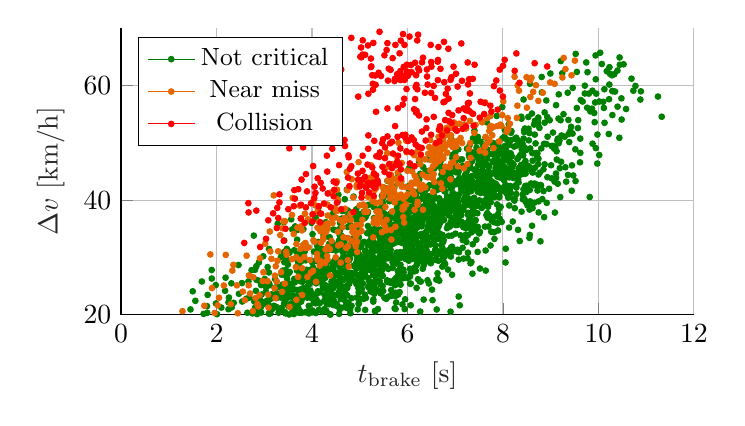
\begin{tikzpicture}

\begin{axis}[%
width=0.6\linewidth,
height=0.3\linewidth,
at={(0\linewidth,0\linewidth)},
scale only axis,
xmin=0,
xmax=12,
xlabel style={font=\color{white!15!black}},
xlabel={$t_{\textup{brake}}$ [s]},
ymin=20,
ymax=70,
ylabel style={font=\color{white!15!black}},
ylabel={$\Delta v$ [km/h]},
axis x line*=bottom,
axis y line*=left,
xmajorgrids,
ymajorgrids,
legend pos=north west
]
\addplot [color=black!50!green, draw=none, mark size=1pt, mark=*, mark options={solid, black!50!green}]
table[row sep=crcr]{%
7.17542881174978	29.7840563596156\\
4.55617151892067	27.3429918859236\\
8.66275590051315	39.5574026533982\\
4.29850967001865	20.7167323954455\\
8.74017277399291	53.4343778342959\\
4.59110156267563	28.2148183421491\\
7.36101980852965	27.1543516128806\\
7.67667922333516	47.7437962920532\\
6.58486890470633	37.694048488668\\
5.87523654902274	32.7343216842973\\
7.65867354283969	41.7680681592722\\
6.78066496045229	30.1765817490313\\
3.6891463837418	22.444810489471\\
4.49462696894261	23.4052201152934\\
7.06778987702025	45.0226661168115\\
4.9517939205747	31.6219900091734\\
4.58348578855334	24.6255542250829\\
2.69114098244439	22.9716906826664\\
5.0827629776924	22.753381378235\\
7.16490323517043	38.2909313088035\\
5.05517998373386	29.0741411035104\\
4.1689735591204	23.9050366988375\\
6.45721048463881	36.1589221020025\\
8.16369835753466	48.1632366776267\\
5.41630431365946	25.9324230615407\\
5.01553804971997	36.8040390357654\\
3.11346868071245	20.3756462944282\\
5.57662510013303	25.7006389005336\\
6.05698977365607	38.4087997508758\\
7.45216940133372	45.1645844533616\\
5.2999630636237	27.0318275096857\\
5.71781062872398	39.7205115449718\\
5.53785021559835	36.2100333953243\\
8.38349275039509	54.5558119073953\\
5.04628408811557	36.8651183148702\\
5.94322308061429	34.9914017549236\\
6.92474014205025	42.0953368951764\\
7.69820973212272	45.7566577058937\\
6.27007331530374	40.122008976608\\
3.68656983779073	23.2369655270838\\
4.6925611643958	24.3250784701848\\
10.4817600389956	57.7570529887008\\
4.83907305917774	26.1265851106518\\
3.11176750314958	25.147124247341\\
9.41105661803418	52.0458851235647\\
5.43882102474495	32.6056016869758\\
5.66830908249206	29.9633554821764\\
10.7759600924796	59.9290931930817\\
6.09560837753898	33.9087164098207\\
4.63876846640512	29.0208152142491\\
4.51280580696867	25.1654054516445\\
5.5146791318396	37.3695455006271\\
4.52940898991141	21.6248291767967\\
7.63956475075811	41.5160924061271\\
4.82867924704898	22.8667488973688\\
7.37198858417559	50.7990561779075\\
6.5526244127272	34.7880588807784\\
5.65746374841106	23.280495722366\\
7.29070573415116	40.2701984317555\\
8.37770900818681	46.0477259198795\\
3.901926792098	22.9746407489985\\
7.95836065427418	41.5536356416854\\
5.30707960449246	24.9991872290967\\
6.55006367562332	39.0730722251294\\
5.90037892100342	40.4815181450969\\
4.20720676400914	25.8696878475552\\
9.71610443472294	58.6090204591487\\
4.7867587052075	32.0942700330191\\
7.30552925122118	37.4275334748794\\
8.78625930763551	42.6308427933125\\
4.93394154394281	33.4447123508943\\
6.94001243796454	36.8993857588221\\
4.94303979777326	34.9256864072869\\
5.36003988901591	25.8916810040161\\
5.00326905336198	30.2587920634024\\
5.07959003136865	27.2373335733906\\
8.45815633451856	49.1187927369302\\
7.81629720093892	37.1067237849439\\
5.33600399673104	27.5853175855607\\
6.17547160683213	33.107596020375\\
5.63954364165616	30.791547822926\\
4.77170728790178	21.3073626790657\\
4.41416013112751	27.9685918780384\\
3.93354625560901	21.5325132212745\\
8.13448262875451	49.9688602008514\\
4.75701459060955	37.291341425726\\
6.71235948305944	33.826104827799\\
6.32035236851526	28.0057318776745\\
4.51778014911949	29.2011497441325\\
8.15794448684542	46.553568708971\\
6.38657502163884	32.7344335562632\\
7.75363961269089	43.1609594072175\\
6.22245658222502	36.8691487083002\\
4.12668705949156	32.6973532259233\\
7.46980204843372	30.9491990402061\\
4.93600009929707	27.0202090977503\\
4.788888254823	25.9876698414708\\
9.66989715735079	57.205190180646\\
8.45504250803507	45.914735622295\\
9.83135147538302	55.4818597251802\\
7.62401073702891	35.3709492303983\\
6.70250246806608	42.1330468790552\\
10.2854548568479	61.7882342000866\\
5.40443976446877	38.2383988192293\\
7.46417672586357	37.7091520932182\\
7.05261328116229	40.4667770110944\\
4.15008881326129	29.7243155639789\\
2.3185407487708	21.2653948215204\\
7.97475686411129	36.1877005773109\\
6.93046698851753	33.8075558601331\\
5.17079043222769	37.9610385906362\\
9.21763758872846	46.6927687545368\\
1.89957756208021	27.7999674459568\\
3.38621654828018	24.0920652859822\\
2.93663254857288	20.3660520354429\\
5.95935223309628	29.7183522509856\\
3.35302884150774	30.1006097650305\\
3.43399860614669	22.3981795885611\\
5.15598657935917	34.2196173372872\\
5.77616283696274	29.4582297767375\\
6.74829580312615	32.6671747665184\\
5.01879829340074	29.3726487609168\\
6.32171819594799	33.6591329158979\\
2.9447322828412	21.8200257339731\\
7.599578070293	46.3640129829181\\
3.85491357471212	32.401866636072\\
5.36777265161089	27.5763837582128\\
3.47376971363152	31.4868077161715\\
5.64178408140898	32.3729750141059\\
3.73790303844732	26.1752361553153\\
4.042717977618	31.0025415004291\\
7.9672800086321	45.9906266585066\\
8.42439898657383	47.7915078198065\\
7.88387203912547	35.9648812900294\\
8.03318569906542	51.1057294963055\\
6.41233239366805	37.4316915692195\\
3.99287758098374	23.4912464055124\\
8.91597246857202	49.7527270987391\\
3.41997031950892	29.1601005799893\\
7.65638809854543	43.105862851464\\
7.4627942794668	47.4862664801261\\
6.97726211368677	40.125805534553\\
5.47453205428729	27.8342673831902\\
4.51699317893243	25.6680874535794\\
3.07124094369921	28.3064366932975\\
7.02192714865712	37.5513662686083\\
7.13910661597048	38.2425807762951\\
5.80307057764156	34.7671770673741\\
5.2723013536311	23.9185844439061\\
7.51711147371981	34.4553673700623\\
7.73268881934024	41.7418945862053\\
4.22622953104337	25.0192271220394\\
10.8896669892777	58.9836604762446\\
7.33177853940452	41.7765629870789\\
7.17803341576245	40.0601563927711\\
6.55356158518646	35.6195037575231\\
5.4431649348831	33.3465850353922\\
5.56055862495187	36.0296471970681\\
5.16385442835041	37.6595239976908\\
5.87286606424578	32.6889071720535\\
6.29795036298282	35.4147645659931\\
4.58924652911925	33.9032494916648\\
5.17986865574874	24.8085406242283\\
4.98247881033315	33.5227773338502\\
6.14491676820979	28.1884060283267\\
3.63916671935114	25.6184016532412\\
4.60199499698046	33.323610446747\\
7.00547062570811	35.6558803997528\\
8.41760746964488	40.1313553871003\\
7.23322625553386	39.0990659814419\\
5.9479076125803	33.8241407290392\\
4.49776472726933	31.8424629453253\\
3.76211603726132	24.3246067097056\\
7.13425741002732	43.2748462295384\\
8.9311501808198	43.9899859611265\\
5.93862735651659	30.3673786433123\\
4.71666719121066	28.8560365552325\\
4.13053888359503	32.0855837443758\\
9.12453481946721	48.5177281600457\\
6.95239246388422	38.7790362067817\\
7.92515548873094	41.9835357143298\\
6.0296745974094	29.41996758269\\
6.3940357001526	39.6521802914236\\
2.91237449371353	22.6314745047367\\
5.71889478615087	34.5199215553203\\
8.87364498436586	55.3026780556186\\
4.35848193081132	28.0354479894329\\
5.92967234401231	26.6999433050419\\
6.07834392514062	38.7177064525662\\
2.25092007330979	22.1472588752202\\
7.30516301061166	42.5093342492765\\
6.96080116379863	46.1273642725282\\
6.2969815151902	29.3610305356824\\
7.79475870619665	49.2805797871547\\
4.6735289720621	31.3747763904635\\
7.39603089232188	40.4011989204249\\
7.14240264862714	47.1154676574028\\
6.84978812486701	35.5796661873408\\
3.75519672763012	20.5995609558843\\
5.74026208897214	23.2537724937277\\
6.12482214859211	33.85670682267\\
7.44739769550339	41.9965471288887\\
3.9783774414123	27.1947680074154\\
5.35365365955201	29.0280652107349\\
3.41855770012371	32.9428930784136\\
5.60666923077253	35.8906221054876\\
7.62487578790894	44.2462059514843\\
7.31445217688998	42.0324370115099\\
5.94195121068235	20.9778127092283\\
6.79019427801194	28.8455933091129\\
3.77208663202199	22.2629962633572\\
9.37663317901187	51.535328999356\\
8.74065799684191	54.4095348020386\\
4.52258810371817	29.3802567872969\\
6.22213024486092	26.1935783930287\\
5.43166853324639	36.7594371022308\\
3.87597826238029	24.2617651876311\\
5.48996154786819	40.3413786346591\\
6.49376365166426	30.5821569863773\\
6.37997034998272	30.6291047444932\\
8.32271705832022	47.4122523502751\\
4.58782282129977	36.0221474177026\\
4.08301284223564	27.3576455963946\\
3.0955182704901	20.1889015624895\\
4.11020069378978	31.9694883060088\\
3.70453628947751	20.9638162678468\\
9.05025143852437	49.4574406905811\\
5.94493929263907	33.1945662076429\\
7.4042618246101	39.3223114863823\\
4.20626164243636	31.4605999368246\\
3.82002005202718	24.6298634940724\\
6.19136064796854	24.6726022324845\\
6.39059087141028	34.315693424093\\
1.45511488563808	20.9159464311755\\
6.17294257096488	38.3219889951113\\
6.58264340971097	37.6494971414415\\
7.68700642817417	38.9032325470887\\
7.96180137312447	43.90624569887\\
6.83694791306538	38.3661523748495\\
5.17083806343689	32.1288016688074\\
6.0153162452005	33.7259580175745\\
6.10317554297945	39.9110030424243\\
7.12681260615716	36.2309264547133\\
5.36247669023686	29.5223618694049\\
3.73872666352261	20.3303744245198\\
6.33126913654188	38.8933863013055\\
5.10527664054673	29.1033357642556\\
5.74064844708747	25.1532082153834\\
6.03510458252575	41.7736066399576\\
5.30391517318164	31.2011702537628\\
6.95606327027634	31.0524843311366\\
4.92781793560548	28.1146418826675\\
4.90860461297827	31.228947191725\\
6.79684860690265	39.8387281170614\\
4.79636717504673	29.8356122536337\\
7.67852560020288	40.3279759581323\\
6.34212229155073	33.7544759428966\\
7.0184605671525	38.5281483970056\\
9.54798444823949	56.0751122566905\\
5.4122111055527	27.2591853279382\\
5.73196375473826	21.1063589989481\\
7.17000204374358	35.2681586167632\\
8.17008637253505	52.0522104254261\\
6.44903605161901	25.440623897131\\
10.1748539262216	62.5058668964861\\
3.56515630360276	36.6518434618105\\
5.96294231053259	30.750333211907\\
2.88783605549557	29.1127088788711\\
4.56527720771632	23.9773609880188\\
5.35605153089222	33.959769623042\\
3.52945819908136	30.8001526512566\\
6.63825358842818	26.2356022936165\\
2.31169519946233	25.4682322520618\\
7.40326214456038	38.8949461218176\\
5.58683756925507	35.0548137053308\\
7.21536026534839	40.4511534212131\\
4.94459038538361	29.4975618290329\\
7.95951315502021	41.9598279905829\\
6.05575665618713	25.380795417979\\
6.08304152040394	30.9058033947113\\
3.28116961842868	35.8508268915053\\
4.57761590660049	23.3621533663728\\
5.72181553133926	33.934665441043\\
4.26637047257895	23.3948922353063\\
4.05360153812254	23.4657623312948\\
4.22772413468253	24.5409351877564\\
7.88849849813701	47.1991171229156\\
6.71407540307728	38.8465423723597\\
6.11081950426018	35.9726891769503\\
6.67824559960906	39.7270440543965\\
7.06548170273543	48.8599538694805\\
5.18565959683553	30.7891163459947\\
3.55948333379429	21.9467495710817\\
6.91591034043259	39.9541918496639\\
3.91947048237549	27.0350528697312\\
4.35913142982043	21.8124325193006\\
6.62785031448926	42.1847712799336\\
7.55200212279357	43.1180134445421\\
3.53481993660269	24.3826517090554\\
3.12980589480615	20.2149668094155\\
5.33232409815367	28.6704973520894\\
5.23891133850101	33.7564652590262\\
6.76172775040391	38.2348769602117\\
6.30301706437754	41.5609648500969\\
8.86055372656214	49.8196033078337\\
5.3411031321926	34.6888237321277\\
7.07464423782156	37.0148116543172\\
5.7762024255047	38.5621163195273\\
7.07437047813131	29.6014875729914\\
4.74019672360292	24.6495100669066\\
6.61021325614429	31.1184895726541\\
6.66209952740415	35.6008223807924\\
8.41214827033464	48.4349044261542\\
3.03433283295917	24.017857262201\\
6.6114246570269	41.736567150135\\
6.28003942673769	38.6187474069286\\
8.32894212558644	43.0718093374875\\
5.11448209052599	20.8250803670248\\
9.74468432354766	64.0273260370369\\
2.84960860628919	20.095286738462\\
5.60004951531718	35.639617339884\\
6.55269384670336	32.9093161484464\\
8.39476173017322	50.1485874398407\\
9.16887800810292	49.9274088514858\\
6.55214052023469	37.4369538452816\\
5.76317556539561	22.1250209714363\\
6.08860075927355	40.4587633022849\\
3.48606078171776	29.409812499709\\
8.86277166810227	37.0158379554691\\
4.49020050242506	34.746510437374\\
6.84970767234003	27.8649729928101\\
4.30226466552361	25.0163939717871\\
6.06930903796308	21.6341887273716\\
6.24511405010752	30.7998149723331\\
6.74562373369763	33.658222821749\\
6.03665106838508	31.6323158506022\\
5.88870936742147	27.4985551034986\\
4.95318875829263	28.6397173863861\\
4.4593890337447	28.8811883665247\\
7.40319629249323	45.3106875953585\\
5.96603221074505	31.8747361818038\\
5.46897537563939	28.3708657636213\\
6.45922217663909	35.8828072739505\\
5.27479618631695	27.6102850309164\\
4.61864482885342	21.2024814443005\\
8.1202243974504	47.6019510992167\\
4.42278438294955	28.1708149554583\\
7.88999818663546	42.4090709801771\\
4.43460700727328	31.5487067585279\\
7.411368596951	39.5200438000693\\
3.1291761856917	23.0194559419868\\
7.55226583162326	38.6949454279561\\
3.75045528314815	30.5387958058574\\
4.70048454564996	27.2660141741432\\
6.9081178633834	36.2147131120369\\
10.2439628415331	62.0333387625376\\
8.84973219761408	41.5727251514518\\
8.43109610256435	41.8920741724329\\
8.23000347886425	40.0631632207148\\
3.09704663516278	21.5946101344534\\
7.8463244135177	41.910862067676\\
5.7611340964819	35.855821598588\\
8.52949184263144	45.9782315633992\\
4.06862371169535	26.2688768016964\\
3.62686269332485	26.2225114140548\\
5.81668277775605	37.4141798531723\\
7.07781176503375	30.8933398047517\\
9.02170942864637	43.7889857755818\\
3.86800073577509	29.4764612192487\\
3.68899596271165	33.0933017836144\\
7.35951492252799	35.5724920065263\\
6.04112725385395	41.6724502955127\\
7.20535814395048	44.3615729190993\\
5.11736678278624	31.1547687732665\\
3.38881677658467	25.2874340763547\\
7.78972214053095	44.6459957441286\\
5.98544117441349	38.0060524066343\\
4.4309833997848	31.32659215954\\
8.4748073045877	44.6146760205885\\
5.29173473425043	38.8208008287126\\
10.2177325239555	51.5349304819855\\
5.7257857833612	42.3366727936178\\
6.42317062183112	40.6694862039918\\
5.94507221955136	37.4406061280572\\
9.87750755307775	49.8491819838816\\
7.5417260053252	44.561277217521\\
7.21405461275827	35.7969213481083\\
6.23294341721596	29.243622886967\\
6.70138252903665	45.809666661216\\
6.7725353342839	41.605529088\\
2.79138266205743	22.2989613058678\\
7.0957549790219	36.121732834067\\
7.98579724667135	56.2478021715229\\
2.53302330108576	25.5101272779538\\
6.05407380766323	26.7528976171795\\
7.71568570308972	37.3057392622366\\
7.24672907593032	48.9749573483891\\
7.74385154436831	39.6233872184205\\
9.52170384078956	43.3197974036011\\
5.91112964767285	35.805144557752\\
5.22979119781626	27.7898449339248\\
6.20917690416232	33.901110583155\\
4.32637519295117	27.4396647395034\\
7.53014003163886	50.2003211942768\\
7.98507987161634	45.5440216261056\\
4.32845994350656	24.2327432965805\\
2.78196078017326	33.7996647975799\\
5.14482871495393	28.947438089623\\
8.24994100666409	38.5783105074688\\
4.21596184490506	20.4623400777211\\
4.04646274146554	26.6470376505207\\
6.04096975560108	30.5639512754031\\
4.60880006818596	33.8467799082429\\
4.63757305280383	38.0867318426068\\
6.33697384982385	31.2120215109531\\
7.78441169170562	46.7671393514595\\
7.20721090861714	43.597140018342\\
4.5699356232484	32.3887636296077\\
4.50978818207528	31.556538006976\\
8.71207391778701	42.6873599280465\\
8.44421497637396	52.1458723749165\\
7.68792280353319	38.8467328595469\\
5.62150440927707	40.7051116624609\\
6.25158776848379	40.1246506807245\\
8.12272098204435	42.3606563060082\\
7.92039261301364	40.7256682109577\\
6.42319965128977	34.9300558859356\\
7.96134015567447	41.9909636455143\\
7.34731068123095	44.1739329542698\\
7.1057567112317	42.5788524942555\\
7.76681226090347	43.2634299203937\\
6.91035758632009	38.0950551550435\\
6.53058675694252	44.3676205830318\\
4.73298792320254	31.7682368412293\\
6.24924215876347	32.1780415714249\\
3.60291689865075	20.5276341873946\\
9.94564309667963	49.0728863723256\\
6.02709756493983	39.9644430385259\\
5.11405237010941	31.0478880925646\\
7.93074372293371	42.0768186023932\\
7.09557508340368	47.0596126609049\\
5.6887932436752	29.1423098939527\\
7.22516512618951	33.9863009248387\\
5.65945528417015	24.299485674374\\
5.69008926984983	34.64563168042\\
7.24916969081989	35.2341054958049\\
5.68744095458193	32.3407545151222\\
6.04026306477362	36.0811675196649\\
5.23978971301459	34.8454823372668\\
6.19968638769796	33.9117100491414\\
3.04110210341262	22.3596242822154\\
4.62527858151915	36.7805261940361\\
6.5145107508085	24.3665380418748\\
1.81479850866855	23.4478586309557\\
5.01931447208551	25.0826674865346\\
5.83286248751284	40.475373718463\\
2.62592545102814	22.7924609748823\\
5.3349821397107	35.4980746168824\\
5.4916456642168	24.1412963774867\\
7.8466130478788	45.5967564312283\\
4.44620495562962	24.6315565660921\\
3.90624794887589	23.1460510898257\\
9.62118114231377	48.2341254562429\\
5.8435373936544	35.4687238291588\\
8.62322188403881	46.868458012148\\
8.59268204517169	39.3642560446982\\
5.95484523224951	32.953466390687\\
4.94705703233706	36.2920268291096\\
3.43328850684677	20.44806838957\\
2.10101169821499	21.2350997870535\\
6.11894914536088	32.6301253597654\\
7.31154939657982	43.8868858904845\\
5.63484263415106	40.5944724396381\\
6.42134567848612	33.5379382465486\\
8.13232119612162	39.0589485200068\\
6.0081254813931	37.0227181231335\\
8.56307010055464	41.76783015681\\
5.74498896200942	32.5535903930905\\
6.91629623013448	50.696512771123\\
6.64077088173728	38.5677830685016\\
5.31519208121506	23.9131718372744\\
7.6929219236546	40.6840154153145\\
5.04873436768127	29.9701242137804\\
6.72694163080127	37.0822362386695\\
5.442116048706	36.9772704985484\\
6.71730729027999	38.0962566976199\\
8.44633738534603	51.8575284019863\\
6.50620043645087	36.7758081443467\\
4.67346318160402	22.5913817711686\\
9.5707870741251	52.5697621952002\\
3.49678000255438	27.0950103612653\\
7.97900169104463	48.4146798252887\\
8.3942588066219	48.8671597897443\\
3.78179672900596	20.3142055516888\\
3.96710935076718	22.9525861822054\\
5.61570231200636	32.8516969459758\\
6.0542261025901	37.9921976760548\\
4.38606285683709	20.0070096779331\\
7.09596209681557	21.632120436796\\
4.73188966385255	26.7929943735055\\
3.10051632969312	31.4738581458076\\
4.75043506303595	30.1511802679789\\
9.97928930315102	51.439397640065\\
3.76038769689492	22.6908739926812\\
6.26866473825459	32.010790255949\\
5.77855952654012	37.4705133070052\\
8.07741808036768	47.3458773446972\\
3.66542392375055	21.2686945286229\\
8.49770028176175	41.4336385176696\\
5.41420287177628	36.5663405185817\\
5.71681535311847	33.6085282073231\\
5.86656426628735	29.9404431255064\\
4.00439934009854	20.4100823447137\\
8.0979334184071	45.4596369003311\\
5.47513908499311	28.3570934870024\\
5.85398539255867	36.096631854225\\
4.76139926820035	22.0701460190551\\
7.67962577543504	36.9158385249093\\
6.54385356691989	33.6818047552963\\
4.91417790702055	37.3176000151006\\
8.8747247776963	53.5099182739146\\
7.93211519162982	36.7391303660704\\
5.23106141389185	42.9754040499058\\
7.94848084038547	44.691989288455\\
7.33696425786854	44.0166012764257\\
4.85397347737436	31.9957622729715\\
5.76479795017289	23.3731456910151\\
8.5319243178549	54.510943531634\\
5.34693050640027	25.8431072356195\\
8.3378961220844	44.2767398710389\\
4.64613516941356	26.0318461639037\\
6.85806205708995	43.1407699649197\\
9.16448740316802	54.2232046624774\\
6.99073615586064	46.4078621889453\\
5.86622979244378	30.5359042548392\\
7.90884140053383	42.0834212661326\\
3.44783079954376	20.220668125234\\
8.46055271735804	52.4900851959543\\
7.8220248226081	33.215517725873\\
5.64209216955302	25.5670412898997\\
8.12104478348325	53.2665728117348\\
4.97922777354278	36.3412953506556\\
6.59739851024052	29.6671416596362\\
7.66592045778124	47.2025812593524\\
3.68627354211855	27.700722844722\\
7.32038957435696	28.9617950265793\\
6.40392465546409	29.821907358811\\
4.3610139436388	32.3815884782352\\
8.38998241086905	37.9784053303401\\
4.30114295691962	22.9680248006975\\
5.31216918663138	28.6055118328903\\
6.326553949596	40.4316394634358\\
5.04216348191961	24.5369812923485\\
2.82608354994815	24.1568318311722\\
3.74458416688728	27.0386910179824\\
5.88548329873623	32.7583731105159\\
8.3522317870041	32.8519293345623\\
6.09002344999959	35.5893340347221\\
6.31879007518386	37.729156566448\\
5.81347679758627	35.5810462601131\\
8.2454764798372	42.4148864711117\\
5.24415015907931	33.1079384551637\\
6.37461755306428	34.360733637997\\
3.64644080185008	22.2311727145889\\
6.48602629481414	29.7079347223509\\
5.1900842896846	34.4554426459326\\
8.88237687226562	49.7992573525462\\
6.0906303892375	32.5830624348865\\
6.2683140332123	44.5944284201439\\
6.25241591100075	41.7118865361785\\
9.07331624014293	48.9785794476222\\
7.30746074247224	45.9258782338857\\
5.0158851935554	29.3635194081444\\
4.40244415066842	22.4267229093791\\
3.69597507312824	34.8104615320548\\
4.08717325516018	25.4749210620274\\
5.03993601946216	26.7589276717703\\
8.40881472865355	44.8663186413644\\
9.13937247569177	50.3686443561015\\
9.02044316057559	49.4421417459307\\
7.33971840693861	29.2009156037702\\
4.7628940874598	26.4128582108168\\
3.56381171386785	25.3970991393666\\
6.55210363384346	36.5809931381307\\
7.80883807460977	46.5657038397627\\
4.53198311322115	28.75417780049\\
3.67373420793627	22.7756685310063\\
7.47786477586144	42.0159557815564\\
7.75509326452321	34.4791835826516\\
6.26397387094245	36.0508301740359\\
7.28689491049442	47.9931519376614\\
7.34564641110031	34.3831107393621\\
7.82177414032822	44.9072584319283\\
6.82822829408426	35.0994865458788\\
5.40667453056209	29.3851308990261\\
6.42838385238262	38.5677182154384\\
7.93378242470107	46.7549584903351\\
1.98473426178495	25.1671550099981\\
8.00936663219289	44.2332816952332\\
5.96880829905351	33.9294870230281\\
5.28574027716563	22.6480305674359\\
3.60899440056678	20.2243600389813\\
7.00520919362037	34.1415764642236\\
5.62929340828647	25.8030897508659\\
5.52679003758852	31.9003422551683\\
7.35899577082414	42.1215611550957\\
5.62035799728796	39.800236562303\\
9.15029570643025	50.7207684403125\\
4.58140710931494	20.928536747496\\
5.82120801846429	30.0259165365472\\
5.44437011631256	33.8836012221038\\
8.05121326484537	48.9830946601745\\
3.2633666164334	23.7122100401807\\
7.40362477342404	52.1346514699081\\
6.43255209806215	35.4634127292517\\
7.05794779746473	39.6842232904584\\
4.27735345136768	30.560944731293\\
5.20653334553955	25.2361995233116\\
4.24964529952202	20.7612414904825\\
8.62297188071945	48.2208606132894\\
3.36463917961354	26.9791276852681\\
6.35057988376672	38.4303572874981\\
6.98641440537924	43.152050211925\\
6.51828877271544	36.8599531955988\\
4.00831248292395	29.0497212285753\\
5.28074682575251	26.9099087117796\\
8.4336505772631	50.724735530227\\
5.57993071168223	34.557181011522\\
6.420119298322	25.99972122962\\
2.994397347416	21.9601214346388\\
6.66658455332973	25.9239236733964\\
2.25152253306015	20.9474592271864\\
6.31320168374916	36.0198168860729\\
5.09878502190543	28.3884684607273\\
6.12906378767763	41.5139493098343\\
6.57725566181666	37.0481926995251\\
7.12920283476989	37.394400748678\\
2.90118464820837	25.9041542737385\\
6.52225169649616	38.328333740549\\
7.30784940126072	36.6808000042565\\
4.73464732171813	21.5354055204228\\
7.06397917011548	44.802329299755\\
1.55747818122806	22.4146114884353\\
3.78067482981238	29.3717504873335\\
5.1745583400352	26.4094879873197\\
8.0859847901634	41.8568924796316\\
4.74203993018583	33.3713662500083\\
7.65924067364128	53.5855365305475\\
8.50458884187947	42.505105385268\\
10.5797374759122	55.9015760390125\\
5.45708034912636	31.3585852001499\\
3.79326876649595	22.7824981461484\\
7.50370508013745	34.1807189745496\\
4.41582261618886	22.8489353718385\\
7.27131532641847	39.5280872566563\\
8.76535534009546	52.6146565950323\\
6.20228977635556	29.0471429631645\\
7.45527045823424	47.9791719475829\\
6.51604093587515	42.5973162092244\\
8.01894690260357	45.9168137927601\\
9.51644904956237	48.8624202641107\\
7.04710142455011	31.3373705641472\\
4.93000660769546	25.3569835410517\\
5.61880972610577	36.1503153820716\\
3.75121478219557	27.9343578971092\\
10.2925702795965	54.8375856045967\\
3.94214271474197	27.7796793928868\\
8.78546307047453	32.8024093124473\\
3.03921701986848	24.8159475020399\\
5.57201682919513	36.2481185811639\\
6.80580127998244	38.0808200814448\\
4.79834878847352	30.7809901573207\\
7.87006499788313	54.6820018649067\\
7.6379500042382	31.1957850326255\\
6.38530296323201	37.7580083505529\\
6.19709972805319	36.8939403922434\\
6.17714492600811	27.6357404594036\\
3.22914813440295	23.1761581280235\\
8.43133366797614	48.562313858937\\
7.49055745913483	43.9119540656532\\
7.53087222072645	41.2519968303713\\
4.74998620782273	35.3087452355985\\
10.2233059471038	57.6087430506238\\
3.7497784397404	30.3711707230317\\
7.37296859448639	43.1759126696461\\
5.60516594797888	36.6239907222728\\
7.57771016099281	48.6166579193782\\
3.77967037082163	24.4131194846757\\
6.23632162105195	30.7172004306575\\
4.52693455129985	29.0664058725293\\
8.57112264758554	49.0116862408809\\
5.61061239447428	31.0206092731686\\
6.28717163837225	37.4149714159172\\
5.83569965540956	23.9365281353906\\
3.76989031955172	22.432170299756\\
6.16568343694624	39.2832512732874\\
5.35972337248804	32.3844342969023\\
6.03192339564236	45.5615794043018\\
7.4504129756562	42.5853172539136\\
6.89537802279736	38.6460928463893\\
6.19885689001415	36.4818926472915\\
9.20088077963985	40.517874415065\\
6.0519072608764	35.5998413487902\\
7.05523775837411	38.8346331303497\\
5.69383431954234	33.6885636148518\\
7.23826639587508	35.9707135129824\\
7.63489215914629	50.9270819994435\\
11.2475517557364	58.0751207241178\\
4.42253919944082	22.9794772868639\\
4.77728567753222	29.4813147376336\\
3.73280727981182	28.5766061004651\\
3.93630448136423	20.216481543137\\
5.78085348117761	34.9104148225746\\
6.69010597485695	39.3641296647878\\
7.68141707725299	42.7587735916722\\
4.03596890676222	26.2906516549569\\
3.27755957971557	24.9280239069321\\
6.4545584463195	42.5947932627942\\
4.97501915538947	29.2062057117673\\
5.76623577682703	35.0531356462039\\
7.073311707924	23.1593178184291\\
7.91104242949082	48.0122509176963\\
4.21750128804526	28.1223696461486\\
5.82535111553851	40.0912047087848\\
5.82426915291989	39.1131270067018\\
5.12968424242789	22.9230375533293\\
8.6706294464184	45.6579096186682\\
5.87677631249708	35.0758475481754\\
9.11099003963389	44.6328289468001\\
4.61294094324659	25.0096154434865\\
3.68977422231539	24.3098783421244\\
5.00338810625076	22.7841095606888\\
7.7980976899577	41.6439995901896\\
6.36219786463535	38.3459078906773\\
8.24576029539488	40.2667729184249\\
4.56329343248571	32.8933294578169\\
10.4486431777023	63.6232400652706\\
6.79195036799312	44.5781063486938\\
5.13781916488848	30.7454025783041\\
3.82048682200679	34.9433870329957\\
5.41138304615306	32.3453580673341\\
5.4352941942632	34.8477445210308\\
6.76172041444198	38.436846463355\\
8.17331224651872	47.6632011384371\\
7.70913040029295	45.8544710108134\\
4.1355905338717	38.6662138132017\\
5.84514028785569	37.5093147096662\\
5.27260074373922	32.9715168055751\\
2.64717464757062	20.3326942105416\\
3.77522811180902	27.6762311721738\\
5.19935939424121	29.2762988070088\\
6.49506455003263	38.9208197255578\\
7.94716448923618	44.2438278700749\\
2.73413492661044	27.7584666930621\\
5.80693072689645	39.7891571047442\\
4.30965629551718	28.9932024467811\\
4.3166487787678	22.7520290555171\\
5.36790150219903	27.0554523453183\\
7.42566564463216	44.2847379504855\\
6.69199605748883	42.8906482841464\\
8.40921844281225	49.0600936702217\\
5.8100260281821	37.3290292537618\\
5.54810645579192	32.2852830862346\\
6.07024757509026	25.4280232681981\\
8.18539844920877	44.8213969795097\\
4.44678032470318	28.0521603448908\\
8.00570382922735	43.7712492432542\\
4.72571331985359	21.1878257096843\\
5.48282552789531	26.7812664507067\\
6.80040281223094	43.2016330802302\\
8.11788667263106	40.5362504446616\\
3.45267764698639	27.7980409125926\\
6.33217912045212	36.6706707814546\\
3.89954408264909	27.0349371316333\\
3.67135376989665	29.9123977853387\\
6.19258821164542	28.6483486530747\\
8.05889749784052	49.4997724883553\\
8.93543229370594	51.0578773931159\\
3.84569170203145	30.9856446592387\\
5.7725698309902	37.8582862866736\\
7.20831008759234	33.3969100824998\\
8.02608982640239	47.4004440987861\\
6.89296464334636	39.8538142318269\\
5.41047847194922	31.962105031751\\
7.01348383625728	45.4158962186226\\
4.21752099698967	27.25225931632\\
4.98280540306927	24.7264448144852\\
5.76066070813296	34.8477815305008\\
7.48373500269025	46.2027318985649\\
5.50468638222321	32.1179514033132\\
3.8172924510877	32.1345411827342\\
8.98053109361966	53.9318132188444\\
8.00340393622437	47.9712503514754\\
8.40028334045511	44.8718337407989\\
2.01007691805792	20.0844218205235\\
5.98749725945956	32.2398061611926\\
6.22161273074207	36.0656898389567\\
8.17556210985915	44.7531459666773\\
4.26516968606739	20.9803003763753\\
3.10392038022611	22.6685610950041\\
7.17349972741822	33.2543124418787\\
4.84027662200453	30.7406462376692\\
6.93355747475204	31.866267104734\\
7.1588083907579	46.0036782102062\\
6.00277354490565	36.5039934075981\\
4.14736246399941	22.1317068204502\\
4.10392839122531	23.6632365419863\\
6.90639804319692	31.2288583867254\\
6.24666650240434	35.5325986967064\\
7.46629065912856	39.040725748001\\
7.10048177692133	38.8334427457697\\
7.44356012814818	45.3197261029659\\
4.47464059206673	29.4935492104258\\
5.40592889792229	30.0066814496536\\
6.88844050419392	35.3750443654662\\
3.22799756598167	23.3935550074817\\
4.80131987200518	35.6675598020322\\
5.24447964964808	30.3901798191042\\
4.98315479243133	22.0010561667637\\
6.75803694772352	44.4794619240178\\
4.71336405574662	21.7423540043195\\
3.15908108359027	20.9507732022482\\
4.74056425123794	28.5017734999873\\
10.2914555551636	59.0392140742143\\
6.16221779117344	40.7337232266607\\
7.7140073686164	44.0862670692476\\
4.25257456205321	30.1295195026994\\
5.28421469016412	33.4402657295181\\
3.41349262108728	36.1228910199553\\
6.52989137514493	38.1604673340293\\
4.45227698270712	26.5263211550694\\
5.71516996998812	29.9806999046207\\
6.37274600572267	33.9656258000742\\
7.43383681028533	42.0635074417822\\
6.0790161876643	27.409893555552\\
4.79643684889573	20.8311963630007\\
5.31903181936133	20.6350017759149\\
5.13101250397329	28.3233711912677\\
6.40119006943095	31.2291988654584\\
6.41309142220431	42.0263737142291\\
3.41566409680107	21.9610590200588\\
8.32562798269215	44.6418037128523\\
8.28114561028687	41.0510771259326\\
6.35742187696382	37.318060042029\\
6.27169808121843	32.4573359727613\\
7.54831323435473	43.8765892580848\\
5.94618135709185	34.4401593141572\\
4.49294135195264	29.3537552074052\\
7.24208906948612	45.9722007562762\\
7.08666001657472	43.8354422032379\\
9.19094446506597	45.5631452833338\\
4.78001741647944	21.3056900367774\\
7.47381615227104	35.3280381885127\\
4.41744790143343	23.6429146408275\\
4.37157250494327	33.5116952396705\\
7.3460474430249	39.7236565034026\\
5.46415073257986	40.7268435624765\\
3.43691261161083	23.2181964895368\\
4.5958579590992	26.1439775323881\\
4.51700182455796	21.9050891356415\\
4.44196834351733	21.6946972571087\\
6.81346544314543	38.766777227183\\
6.68114260629106	37.8608641411901\\
7.48313932241345	47.6168559075706\\
8.28308676498517	42.1828961861774\\
1.90140849047962	26.3049614053053\\
4.44346391544187	28.6627222975656\\
6.60141202713509	45.8564845399803\\
4.51047362652761	31.3659959310413\\
4.23520946013483	26.198576320525\\
6.27941127622082	25.771981331217\\
4.70996281759974	28.8081874321907\\
4.677062092256	32.8419798186194\\
7.16741690014364	38.3305094155081\\
4.25664961865369	22.4071397309986\\
7.67402755206388	48.8137272409645\\
4.89305539525025	27.2225506811777\\
8.15218450891519	42.4607175631745\\
3.65495680662325	20.7870557844065\\
8.8489929411937	45.3688260159183\\
5.06720344668222	32.6294908976171\\
5.32652117895025	27.4458501402897\\
5.40856501679894	36.6586883369463\\
7.92310520131327	43.9719559086976\\
6.12980305773245	36.9347543059044\\
5.31481248623552	29.0114107482731\\
7.51021593063659	46.9771234714567\\
4.89643993043166	25.9537065120406\\
6.65405027853465	30.9733928460934\\
7.3168789086777	35.8942912185882\\
4.62004260244313	32.0546391505\\
4.8478634455821	33.2938931077551\\
6.58347106220673	29.5993160957402\\
6.16365043525797	34.7397190858887\\
4.64627249872685	29.955359427711\\
8.13081914061151	47.1350343442652\\
9.30738546412553	45.7285687428498\\
7.98917731095664	50.7944902553061\\
8.08181876889508	48.4148404467554\\
5.25210457919873	33.9511498219405\\
4.49130769989563	27.356800478117\\
5.89409596706032	21.7923492307509\\
4.24600313830852	25.0767067261244\\
7.19689354910245	39.5606737623484\\
8.5681175122922	60.3010268869632\\
6.76484257867197	38.3185694964428\\
6.24618181009915	41.6020279347182\\
7.33938143979905	36.4159949390731\\
6.64270702854138	34.2737069877844\\
4.34820327193217	31.3171051201724\\
5.52101776728361	42.151698669924\\
6.86561602364184	43.7809730554833\\
5.27289292562747	29.6245534136985\\
10.0375263475674	65.7190156045244\\
5.54300059835722	32.1267254215531\\
8.08037788261653	42.5410972611489\\
6.62123521776909	34.4972211253034\\
3.52087060894167	20.030657466218\\
7.51951807633611	28.0512632885478\\
5.21573134173856	28.1419702570809\\
7.87718191137296	39.2439154722077\\
6.94661201380208	41.1605546971738\\
8.68349285715954	49.892187360919\\
6.37156637993591	40.1088520616623\\
7.35438359534895	46.8167357742542\\
5.92060588596575	30.943486385209\\
6.067752412867	32.7405272479207\\
3.90898093640408	24.902827470419\\
3.47895180397339	26.2289021250162\\
4.73236357754052	29.461276296158\\
7.82022381508465	42.9519368345538\\
6.17575387536972	40.985029900904\\
5.82541451402693	40.2881041790326\\
3.67254595357104	28.3180414245104\\
6.11600075675187	36.3705802762628\\
6.83301040937239	40.5343235260577\\
5.12995938696856	29.77040898535\\
6.68876858023633	36.0690502926074\\
7.62842075463876	47.561181049998\\
6.11842997264012	33.2832827557961\\
3.3008475388838	20.3438949344074\\
5.52534275462553	28.6027337307192\\
5.81568163178157	39.6825340136732\\
10.3478867928708	58.9425736724616\\
7.26645808515385	33.8798359271134\\
6.72067658066545	30.9093987373024\\
4.53808661221877	25.5741269137501\\
3.70496150476258	29.2608599970684\\
5.48787580275856	39.4676006309577\\
6.96783321062544	46.9624087767617\\
4.68658088257705	23.5403354492634\\
7.29964490784378	47.4702311645179\\
5.99694778785016	26.3789394488092\\
10.7319705733035	59.0894722480368\\
5.66476181422201	34.4165264259748\\
6.3945702229223	37.1118715454637\\
7.1546101789243	42.7813474724581\\
7.5758322868228	44.9941540957407\\
5.31353609258134	32.1273972635071\\
6.02445621333767	30.9257508995093\\
6.15019433245959	27.5818620881782\\
7.26975396940592	37.403383997381\\
4.92149023485538	28.9503266446997\\
5.03154269319925	31.8605318115704\\
6.28061292062174	36.7347549458292\\
6.37123749626381	32.7294393505447\\
6.77852321250806	41.6045547756453\\
6.05516857007895	28.0118415495428\\
9.95411599923209	58.5769666629048\\
5.76057128793438	25.9946063444841\\
5.19754304023211	32.6737693653292\\
7.40822270829578	48.1562680070204\\
7.44222438685424	33.0726938005096\\
6.34196913785351	36.8673480060143\\
6.52191750768557	39.8872341614698\\
3.92736864819142	23.2443709640397\\
9.46229503298064	59.5873344902322\\
7.2143858886975	42.3185400220054\\
4.98584725089099	37.5580884812032\\
6.48183974726597	34.7456682041404\\
5.57342198354605	25.991762707588\\
4.90318319710528	33.3679017404271\\
6.31687562847981	37.9068734366787\\
4.89235401939025	31.4651997148529\\
7.47258903990853	41.444729907921\\
4.95932182278665	20.9170938856074\\
3.69741764951045	30.5850210215024\\
7.30485152588759	45.6004099688949\\
7.37973585781381	35.9101646505892\\
5.8145641402083	44.3291381566725\\
4.30063436555642	34.9232361804425\\
3.92529340183169	23.5629641251943\\
5.31576967872888	31.1957638306055\\
8.74436724745163	44.4647949210737\\
6.63666594940037	37.9777356663648\\
4.37836644079673	20.0655185602238\\
8.15106260417856	41.4166988993219\\
3.82983713308375	24.1522178048398\\
5.06061765539339	28.2360893093308\\
8.92942163361689	54.4949072266602\\
7.70176844996283	48.1050869423921\\
8.53791623328932	45.7791865801404\\
2.17980286753618	24.164772580308\\
8.81534068935874	58.8034613983225\\
8.07809493578189	44.1300496082563\\
8.4661401062089	42.4621972101846\\
7.33421751867808	34.909704330478\\
7.95203539388208	38.832620511465\\
7.1590681426497	33.0139980007818\\
4.67887043117117	28.8029878614702\\
5.35213248997874	34.4223078467986\\
6.17118176678816	40.8739182197322\\
5.9235806428055	39.3921171554111\\
8.24683577540901	50.6697045071312\\
4.6717042796087	31.0889802944395\\
9.20836109857442	53.9476784719627\\
5.00230019945759	31.7526778629631\\
3.93261299046475	20.4623442687381\\
6.28529677230641	34.0650860379145\\
9.91239740750155	55.2008213203335\\
5.17983355228911	29.2333152607468\\
8.39017271652846	54.2035131268195\\
8.07504721984828	48.017494326598\\
6.56530387113291	33.0372743538217\\
6.05140345524215	34.9950338271401\\
3.89555439174418	20.5266630002332\\
7.47560032204121	43.1346935895699\\
7.57929628103721	39.7328634784233\\
6.6584764464166	36.2807805243987\\
6.17815999503351	31.1057709490632\\
2.83590382875411	26.0767965106515\\
9.47378048132984	44.291814342573\\
5.55868229317921	34.2407095806846\\
10.1252099699623	59.3536203600501\\
9.81839050506919	40.5344168914633\\
9.1142358194656	43.8899094184876\\
5.47842409827743	30.3413364705982\\
6.48524719655943	39.7771787120167\\
5.8323695088062	39.0808157628738\\
7.41813050766055	47.9380389291428\\
7.88467624146475	44.0925901140917\\
5.29899329674085	36.8636408401646\\
5.25352115100391	24.197112692666\\
3.15026494883424	22.8254755133328\\
3.62583967204246	31.2424008163531\\
5.71387053348949	35.6567799311773\\
6.85893329977459	45.4783296971254\\
3.21754167413732	23.501316312518\\
3.48955590126759	25.3048529165519\\
7.92099374818197	40.4875583419054\\
6.55737854700318	40.805841512764\\
5.06788504778386	28.7549782110772\\
7.55543745372383	38.6387925939571\\
5.91331508336143	26.3887563415249\\
7.25877472566861	29.8526086488721\\
6.99161338329111	39.3834447196413\\
8.54188757674878	50.4262879453205\\
7.59003944545096	49.4221909431914\\
4.2722870108535	33.5863133147607\\
9.12839376265788	47.0687199586239\\
3.57328003696962	23.3008644108954\\
8.11789514108183	49.5743469642121\\
9.36352397665112	44.3940454336307\\
5.29749031032516	24.7495756379509\\
9.97713796570831	46.3781699334509\\
6.22932650033691	30.0247222725128\\
4.97378057601686	31.9570806508037\\
5.92552152407948	38.3749218331606\\
7.07675388245511	38.9001544658455\\
6.71066230128394	32.1765685756286\\
5.96385467525297	32.6332952408078\\
8.91754844927314	39.5133866933693\\
11.3263245483901	54.5495786011123\\
9.44109030308017	41.6313049868177\\
4.74077455296204	22.095153114575\\
8.61561856879685	48.2011414447195\\
5.84590335632309	30.8943471748226\\
6.29462767743789	37.5615242789437\\
4.86867136815135	31.7790955149921\\
5.03389665593413	24.1769788890895\\
5.22582463459279	24.0686552786702\\
5.97381429315368	34.567982551693\\
7.29055539655525	36.4951231434419\\
9.77208002480194	62.328863170309\\
8.79973705727084	42.5344412282248\\
6.14942376214124	30.3532221100451\\
5.795391762842	38.4429952840625\\
1.69276355729838	25.789822493892\\
8.72468389976915	41.6666152699583\\
7.60458890813214	42.8199411319325\\
6.56268981466568	30.7286431762399\\
4.22912640824803	26.571260979032\\
7.36325875264037	40.1011169738813\\
7.48974062207082	41.7139228357599\\
7.19770608948359	44.0684483113704\\
10.2985310147703	59.0163299527807\\
7.27005231758483	43.2942988297387\\
5.46417004977753	26.8149848120329\\
7.64417183253219	39.8340550520989\\
5.63462518141696	36.8187330516005\\
5.09653289985422	32.6829444375402\\
7.49689753883876	42.1658245741971\\
5.91584825726399	27.8390804254081\\
3.25222352283845	21.3527755990582\\
6.63015804945513	38.4988560551256\\
8.81197036189394	61.4918595215742\\
5.6377417757137	37.566550728526\\
4.99843650292323	29.8359468453952\\
7.6653682180221	46.1930364869118\\
6.42501486309124	29.3071445918051\\
7.09674382376038	37.3491328706163\\
3.36275353215604	21.1813464084364\\
7.36321824410624	37.4928317070954\\
5.0902590714071	27.4215013671209\\
5.83186957216627	38.5100803721592\\
6.7399187121942	37.4997989662028\\
7.64058535114974	27.6933100886466\\
7.71430098209939	50.0942525388274\\
3.76680096414504	36.7847813251326\\
5.19374311751073	25.9170304252646\\
4.9264582092848	38.3890730205706\\
7.19649899418594	35.8919235779057\\
5.77798045384275	30.8550561696117\\
6.99128016769884	36.2773953938586\\
5.55946108588368	30.7964972757154\\
6.02010112054601	42.142466238159\\
8.66680123251023	51.4283840660168\\
4.08200277784351	26.1202348369451\\
3.4953323718993	28.7343236828515\\
6.88368521197999	38.9926733798258\\
8.18473953915767	47.6543929791699\\
6.17930168820498	33.2218811459654\\
6.19360652926231	37.0777407314076\\
1.9892606040418	21.9486252155673\\
7.23563399339782	42.2451388772475\\
6.60927739093317	34.850233375883\\
6.05877660209999	32.7619928767698\\
4.13959586471541	26.3707104824293\\
8.07367633442622	41.1494487462323\\
4.29249402004739	28.0758376262379\\
5.03930302136358	28.8591791141827\\
5.51105961495921	37.7148539892431\\
3.46389273593112	27.5274053064221\\
4.58845052845898	34.7889010272768\\
3.85896783981698	20.4109322883794\\
5.4298794372816	24.1145403875996\\
4.07907653220932	26.494504441223\\
10.5274700652909	63.7021784013967\\
5.04456484313727	25.5753910633609\\
9.14787629830758	42.8542029261297\\
10.1149914334653	56.0853550898015\\
7.67311551461019	37.7362199825419\\
5.86478915602862	43.0232305390149\\
7.93008147713359	36.305352067978\\
6.90692225175218	44.0184621295361\\
4.6871136089092	40.157358015715\\
6.91003665282874	39.3596328508778\\
7.9054506325368	48.5263859376813\\
3.25691322291542	22.9023091989037\\
7.61535291014373	41.6376347735455\\
2.85341529104045	21.1028845962652\\
7.67455259795188	48.3216594492707\\
7.39964824796102	45.3054539009206\\
6.10114792464723	31.5617821538808\\
7.26334933765508	46.008002717181\\
4.67704122052307	31.9297004662177\\
5.03327270946043	26.6708985939646\\
7.36901093986365	35.181551746206\\
5.96741112746273	38.6298202816393\\
3.44904751734903	29.8737421192243\\
8.87425125362317	46.2485927853436\\
5.2157803520864	28.6382158791475\\
5.0862833294697	26.6758107246044\\
6.1386386308165	32.430130242924\\
8.18196923647563	46.5266132105269\\
4.57819190821588	32.2539163111832\\
7.78110894917784	47.9973862922019\\
8.1332618640262	43.9597894019218\\
4.67427290916834	26.164146815751\\
7.89894911058825	45.3171087113217\\
7.33298509201805	41.552454317604\\
7.23864206934686	44.9527998921241\\
2.80681966445762	27.8267369677807\\
8.21321225246156	43.8637515299037\\
4.02359936952938	22.7341873364671\\
7.15646735716832	31.6692781386704\\
7.46114769794012	34.6181133282532\\
7.20565411958049	43.1790772942594\\
6.56126208553252	45.4896457298139\\
6.58170437090602	37.2819894376676\\
9.32559890759096	43.2172952630726\\
7.48695108733422	46.175560835071\\
7.00285226487351	36.3176018585213\\
9.79983178685305	58.5851794840333\\
9.42842815022417	52.792266599006\\
8.59644763183901	45.0778951834639\\
5.42932633029036	34.0154418412079\\
5.73808569306292	36.8302916383021\\
8.14487380369606	45.2667260786713\\
3.7972929652418	27.8869740313405\\
7.87594076749031	45.6672063379357\\
8.05024628696613	42.6039624611236\\
7.81964681819669	40.5132313137369\\
5.38071446800082	20.9724651147266\\
7.18163030615375	43.2448589130219\\
4.02392907167205	28.206181754697\\
7.5667743455239	42.6725451237469\\
7.60740646450475	39.3979246672924\\
3.59789519356308	23.4109749316213\\
4.93694235663424	22.9714882046386\\
4.87784024932799	32.3410493896964\\
5.95153371900599	22.6837479460833\\
6.54398938780512	33.3728951495361\\
3.36904347794133	23.7400033647373\\
7.16799380177623	42.2572526107055\\
4.72589275570117	28.4029052804444\\
6.50090102391109	37.955394942022\\
5.64322434658476	30.6425772129204\\
5.80514267110839	23.5084946477669\\
9.87414166156154	59.0952563104254\\
5.4483561718336	36.202571860682\\
4.12321362413285	27.7196845063857\\
3.71701250605279	21.1017907511423\\
6.11342007549697	32.5510766046889\\
7.65260393014099	47.7410583534141\\
4.59082697717207	35.0867129909421\\
7.36726209172811	32.2816730654812\\
7.82765993544285	40.8954848574912\\
5.81443636590009	32.7241707565267\\
4.58355318776428	33.8204457167788\\
5.14169034005349	30.5376936548286\\
7.11257151838453	38.1198021546449\\
8.41447148030515	40.9718434700993\\
6.11662595072964	30.3058479296177\\
5.7505268209005	20.9857881066092\\
7.79777515703625	49.947659262636\\
8.23086190054609	44.7580629486336\\
5.91884705099481	27.3945967922483\\
6.44832245781459	45.099418518838\\
5.8271605007618	27.5165065862499\\
8.2605647511648	44.1217998107159\\
3.2270839493641	24.6976820719893\\
5.61606042240977	31.4588839170041\\
7.30417743077193	49.6144900338585\\
5.45810466050957	27.0530270257485\\
7.92476806147509	38.7751927945887\\
5.90554525163286	34.4485307308148\\
4.71673475746323	21.3090927103722\\
6.31232334921686	29.2699530307381\\
6.58102661757189	31.324006078338\\
5.28416303112035	25.6319136024623\\
3.7289160382335	22.2690256929314\\
9.865170723178	55.9576158920748\\
3.01031689441627	26.2386682113356\\
9.18417119276321	50.3792213891717\\
6.70760118644322	38.7666532582132\\
7.90817273647493	49.2528001221998\\
8.96750948784992	41.9741829699229\\
5.85647346603384	25.2323290975936\\
6.66039606800895	36.5075540954817\\
5.00007854711237	36.1703327776562\\
6.45058808127656	40.0004954799162\\
5.42756479153579	30.4185068000742\\
7.0417250664847	37.0311916908838\\
6.34179227365991	28.6143848936371\\
4.10927740784742	25.8281916262285\\
6.59046340493092	38.1738809352218\\
5.99937979896957	35.938434025795\\
6.48977476559234	28.9720683705819\\
5.94209600934227	37.2174985599376\\
6.45404536406796	40.634823345334\\
6.74704080801762	42.9409820996201\\
6.90885933406788	42.0554459629092\\
6.63521703586818	38.3406880785015\\
1.72961474335169	20.1375855837781\\
5.44301525251069	38.6396958987239\\
3.56098381562451	21.2019931366455\\
2.94289863039287	22.2651702864478\\
5.33886802508364	32.2587173369574\\
6.67477347683616	34.157924928805\\
8.62118101580456	38.6098210686202\\
7.44770322815758	49.163151602294\\
4.33815152628256	22.1652972047928\\
7.0762079644939	40.9691034266645\\
5.69011159750531	25.5964299512994\\
7.50867310458811	39.9536208786845\\
7.47578616607849	51.0245791835207\\
10.4436568504053	64.8978882064628\\
5.74894610539874	25.9044293025312\\
4.67932810867418	27.6878247848556\\
4.1856888063797	29.1020187980902\\
7.85183973307027	47.3919170402848\\
6.64639557680875	35.9554205217625\\
3.18161208904605	21.3040374231877\\
3.89837958527379	27.5520738802505\\
10.2284782499331	60.1698200574112\\
3.77698679455296	29.9518763477313\\
8.47138977481873	46.8081447211573\\
8.5686612707625	39.7761302536083\\
3.39288841869177	24.4919913982595\\
4.64317285668256	30.9262572063339\\
5.37752308380302	36.6485433356659\\
4.14558718436338	20.8663808605851\\
7.81571840149299	36.1271132711231\\
6.02691492370537	29.533272784609\\
6.00697070241161	30.3062712577581\\
5.28246983980816	32.3059824711329\\
7.02270773504452	31.0799531612049\\
5.35244096677322	31.8980315210525\\
6.67776616579415	43.4669927957713\\
4.8739008691631	30.7518808114246\\
4.93906894664745	30.2397934087867\\
4.8287944109363	21.5383475639515\\
4.97709480598109	21.8680699203917\\
7.9190455476361	38.4827420535026\\
7.00980523511986	47.1787118876109\\
4.93976851051722	30.8057201469057\\
2.80971250463714	21.2334048348842\\
7.65390699977143	37.3790904424184\\
6.69228951884705	46.6695579452999\\
8.02840516450599	48.058448327839\\
6.40524172364897	32.8755781158345\\
7.74950214303355	42.8150298712135\\
8.73542459225235	54.093395320404\\
5.68851199401533	28.1693978292135\\
4.87176450895672	28.5212592727976\\
4.92402957674595	34.4685881810673\\
6.76480218076166	36.5309734119622\\
5.64313141913723	33.1097215856658\\
5.4375978713614	31.3968097532167\\
7.4935193071904	46.854410990062\\
4.42931778568425	37.5423809878245\\
7.8143128926192	34.3810087296202\\
5.64626350012069	31.3075215193812\\
9.08239239005117	43.2181362148982\\
9.38922371163277	50.1277607892755\\
8.45021928851605	40.2001192951809\\
5.12377874552553	28.2286670388147\\
3.07819330328016	21.9807800588203\\
6.92259385344631	38.8810268166533\\
7.378354001286	38.3057741353579\\
8.11055203664202	49.7508593592153\\
6.21774057783708	32.2145572305175\\
8.15164874093449	41.3656191836206\\
8.06584999965846	50.6489799093292\\
5.464981108067	32.573661757613\\
4.0137519186321	20.7204316239796\\
5.8542474283104	28.2581630651088\\
6.22313688578606	39.5257689029393\\
5.7600796427551	26.399391319327\\
6.08728237768547	45.6965129755974\\
6.37682217981614	41.7206981398935\\
4.48212172897197	31.8634742634212\\
4.30714791082769	21.8914471832832\\
4.83448576987305	31.0388245072575\\
6.79309080335483	41.4608359308765\\
7.61721847759737	44.8856340074557\\
5.47097407052887	30.6954785139365\\
7.86531715753486	42.0505842808236\\
3.71830944379255	28.7259983526629\\
5.68443898431781	32.4176465880387\\
5.4316448924734	36.5223547254465\\
3.61684039236242	24.4545835683819\\
8.99388706701921	62.0906996429798\\
9.2687336791967	54.9920923401181\\
8.55659020569933	51.6931991907577\\
2.25933367130465	22.9863470489204\\
4.63667488066362	28.8451744650137\\
4.04783917832499	27.3476444664523\\
5.24131573940642	32.8942473507215\\
8.56347703249838	33.926888795132\\
1.80141944789277	21.487547363056\\
8.41512750072165	49.7413018535057\\
5.60479131483166	33.8542716242832\\
8.19400372496385	45.7509185369658\\
5.78723810506425	34.8333613155962\\
6.83360491883653	39.4859397629646\\
5.62869594818986	29.9094131820302\\
7.95990202100691	45.1981917840678\\
5.56261043862473	35.1236010338954\\
5.21729400638283	28.1591969935842\\
5.4834204932903	37.6837434615216\\
8.74398573826808	47.2184489005809\\
5.89081716010192	35.8794952445416\\
7.16792959624808	38.6144300429901\\
6.22555112084537	29.332330727683\\
6.16430603028453	36.3242190429158\\
8.02438766525063	45.6502336815724\\
8.30417482989649	47.1716964800432\\
6.86862264233109	38.369037954265\\
6.99744821926806	48.2410754755182\\
5.43891393651321	28.599346650207\\
4.57825597539421	32.8784951341206\\
3.80261456877283	25.7148887181961\\
8.6977085345183	48.2183807404483\\
9.37111766428108	53.9921027541358\\
3.60731496557259	22.9953234867437\\
4.69666623073627	24.8815507821\\
3.9832451843743	25.7709170534258\\
3.65551368299705	20.5290332492631\\
6.15159999091896	34.8855396766839\\
6.84933936759496	44.8887309789941\\
7.67695495998128	48.0050731220981\\
6.96004428435232	40.1248539249402\\
6.02039316409329	33.0154252677131\\
6.38210007917033	45.0806540251192\\
5.19244121515191	34.278555443132\\
8.28865778748594	49.524758110211\\
8.22233702366605	46.262458331208\\
5.60834050420352	23.1662133353145\\
7.68852282901919	37.247573809747\\
7.43281131379409	50.1775280204597\\
7.83295144661974	42.1138833308068\\
6.90989189812714	31.6945338408473\\
6.12507945862512	27.8634502613129\\
5.1712895103381	35.479012199221\\
5.79903549966517	26.7470332537334\\
9.09847453170492	49.0584466637205\\
6.73359172349599	31.6368419323117\\
3.94197544830446	27.3827192921802\\
5.81994044217827	34.1372299903748\\
7.76619344865218	36.3663677433058\\
5.48112836252607	34.0084850830248\\
8.16169893169975	50.4639379192041\\
6.41397415505836	36.9220860029493\\
6.98421079517031	36.9519170662025\\
3.69577174699027	20.4255244569002\\
8.40343860799148	46.1786797403285\\
6.40777750108837	33.0279120917281\\
3.80006436944557	27.2321361107537\\
5.7967863589403	33.0739212354725\\
8.05410075724157	29.1131587231146\\
5.34234283944508	26.8583452128926\\
5.79347131852784	34.9630979812638\\
7.89724332355625	34.695634335263\\
6.63025519849335	27.2272318556078\\
4.70240440993582	23.6981147204387\\
9.00884169872701	46.0804017203595\\
3.39076305639825	27.693962546017\\
4.96150685721602	31.0836632324028\\
4.42316888468151	28.090151444813\\
4.8213693003251	27.2811998650234\\
7.69530262425613	35.3869440113795\\
6.19382036443805	31.2247245043251\\
9.08851940361093	37.8227721393626\\
6.45573505673374	32.3447364642516\\
6.94099757004514	47.3155750808029\\
10.8791410968635	57.5471890219157\\
8.4479687433433	48.8409493792944\\
3.6222878002592	20.1119493549299\\
7.71733297660088	44.8510338921672\\
8.74809123998463	39.7782527939767\\
8.71179382273143	47.6052955185637\\
3.8874755700127	27.8347663088553\\
8.72338895115712	48.1394607230531\\
5.3179282755778	29.3402080492945\\
8.55729673525931	38.3404801120465\\
3.43626871821415	26.8866471175056\\
8.49423570642481	48.7703757817423\\
3.50147832274947	21.5122807300077\\
5.30823999002686	38.7706782799982\\
6.25361151628185	25.8297566590614\\
3.75214874461548	25.8657102393439\\
5.31742394918776	28.8943305897347\\
4.568092179585	20.1480994602029\\
9.35749717791909	58.7349705678426\\
7.31313058634361	46.3163718626768\\
7.09692359341722	38.6458506326805\\
5.76452452051877	28.929634884692\\
2.66929064397338	25.8118147869014\\
6.42586583354101	38.2912587888716\\
4.58943587316549	26.471674626109\\
5.79012112622242	39.0323157599321\\
6.90939150408597	30.1494483065745\\
6.7329421221975	33.9232008438541\\
5.25442609038971	31.480780107187\\
7.01286769765668	43.1141294646057\\
7.12787447929353	38.2184729800079\\
3.92423414090693	25.7300166531594\\
7.90104562147198	50.0936454564764\\
6.7942754359731	38.7956950471054\\
7.11163178961602	33.8575404235274\\
4.17932311283054	30.8137465835221\\
4.25203399243098	20.7401744325643\\
4.04182647765199	26.1946233751891\\
5.47805771419969	24.9924627391651\\
7.28616644684752	41.4887917037107\\
3.25694787750565	25.8087199698757\\
5.62735879200887	31.8651967950277\\
8.14132411233438	41.7892234125058\\
6.73351890971465	39.7338976249683\\
6.28386637091326	38.5178386373685\\
1.80658520357183	20.3227085392915\\
5.72069408903559	25.4246548684405\\
4.5701465675095	23.4507164434709\\
8.31045825609245	50.461070957344\\
6.21738315275949	35.3134582884476\\
5.40497751851109	32.396323218439\\
5.86017768292839	26.2457525559313\\
4.27704381716257	26.4275334494191\\
2.53692516678426	22.2923739835979\\
6.60449388620907	26.1173449462944\\
3.48015357904319	24.4117623948865\\
3.31319241180785	20.7698983791711\\
7.04417984858815	36.0227588231673\\
8.01068178215911	44.1693798211516\\
5.7557917864718	23.8265655950501\\
5.37718760366808	36.4950169530728\\
5.32551892687513	31.9535300541748\\
6.32887798338808	33.2078129195174\\
4.3217262436564	23.5913149174162\\
4.26797071440356	31.0780044288757\\
6.71227732810168	44.4960840634893\\
5.63878624188396	34.0614002161341\\
4.80514908070576	20.2460635062471\\
6.17234900052215	37.3082659375525\\
4.08007954030104	20.2910157312283\\
6.61290092484589	20.9015809061293\\
1.50213713897257	24.0790776161322\\
6.64832660232396	29.4082941990426\\
6.89040684712986	40.2776954881349\\
7.01945113287991	35.6661796777069\\
2.97967376161042	30.1902447542555\\
4.0011178864401	26.472398549528\\
6.81240569398354	42.6139642359918\\
7.9002491916794	44.648878819898\\
6.89714432198959	44.6376155479402\\
5.21692798128799	32.9057112525507\\
7.12955932535251	41.8937054638368\\
6.85413550699477	43.0185518265631\\
6.64575806174672	33.219428235735\\
6.06736735205708	37.991653082148\\
5.2900490075459	34.0904521412668\\
4.07557748709959	21.9702037471694\\
6.39084282686048	31.9302537011716\\
7.90253425525003	37.5943953591955\\
6.58097820195942	42.2852306077846\\
7.42926865675359	36.5062265037255\\
4.68773106773109	30.1465389907262\\
9.52369247195097	65.5235011268266\\
6.10977071379148	29.7569138734544\\
8.02596660764748	43.4434809631913\\
7.37640489945109	37.6318539701967\\
7.24443210600625	41.2632273982074\\
5.04853810864923	27.389396731605\\
6.05118032521453	26.6433563041167\\
4.2854189353062	25.1131494085723\\
6.35181690645133	38.3783425179683\\
4.12040773499432	26.8231372902696\\
3.70416029483955	21.3876175272151\\
8.03947975747474	52.2451490641245\\
3.43975976671033	23.1807992941343\\
7.41651723349637	36.4194790620599\\
4.27167524922076	25.0597061657271\\
10.2316720916463	63.1983465345664\\
6.90597584219827	39.5373745349235\\
4.49850402231594	31.1969580160888\\
2.94581022865945	23.5239534041145\\
5.02204062800448	25.9326908410977\\
8.1099545224045	40.4449822193123\\
4.23934911698427	27.7250785241943\\
8.38266138352047	46.1292308302818\\
4.99437369425491	30.455669514713\\
5.28446300497707	22.2744006303113\\
6.91786172426007	41.9974339955284\\
8.36268703998511	47.8612015366676\\
7.84923874658566	47.6190417362476\\
4.77389125301216	27.2357874948743\\
3.53366820723679	27.4475355803871\\
2.19021324785264	26.4548916256086\\
4.75229867408828	25.2051891671011\\
6.51147202851823	36.2153511378236\\
4.60174369572881	22.7392509897531\\
6.40537211637967	34.5650233762025\\
5.34666883763108	31.2442160424923\\
5.0723980043614	26.610640211971\\
3.22721048130413	26.2097256996875\\
5.68478972561171	32.5851326855867\\
8.64338934030651	45.4958874924975\\
8.10080115385501	41.0603631144402\\
5.86643028690956	36.3877815863426\\
4.18946473217942	27.1800640244053\\
4.4492562267983	34.8466356425919\\
5.89274792574537	37.1700474395152\\
6.87530425023852	30.5925534314129\\
4.10586713620895	29.3356991258807\\
7.54352719425479	44.9605766939058\\
7.0182544303933	40.9110725085152\\
8.62286607512092	44.804873884099\\
3.7671337600938	29.8970884883546\\
6.97345118114791	39.9728614891353\\
5.43769746390618	25.284212582963\\
5.12523519156329	37.0462071504533\\
3.00113436574497	25.2264117265524\\
6.58880695266064	31.0708880447817\\
3.5253870803859	31.0193042161926\\
5.96398981059092	34.939874459613\\
5.44223283249983	27.9673658444202\\
6.99032459709077	43.2678711702086\\
3.64635126302463	35.400744264394\\
6.38307623875862	39.244006429849\\
4.75014166366091	36.5614855831942\\
5.58916750394101	37.3133410553739\\
5.9471130348535	36.2527252096412\\
8.51375671390847	39.0847095375252\\
8.73796978560833	46.2735541385382\\
5.72228297490394	26.0540724019042\\
7.21963533376016	35.1350284434101\\
9.94462067112622	61.0854881089738\\
9.22659009339028	51.2791107298883\\
9.54892901624139	62.3708078215863\\
6.06533833173553	34.5513180364778\\
4.98567264062241	26.6544736833202\\
2.93925056798148	21.4716587841676\\
8.13376904668197	44.7328253190602\\
6.57976588282343	37.6866896070887\\
10.1015688941747	57.1547859449152\\
8.58848123945289	42.9039335753112\\
9.63006771419855	57.463255023805\\
3.58547415708288	34.8867482085934\\
4.75272693442197	38.1793664464326\\
5.10236410715829	28.7690786147718\\
3.42165737256584	24.8253818507164\\
6.51833919413137	40.1372974156261\\
6.71801500556807	45.2744019841247\\
9.21242755365955	64.2593895427468\\
3.75489412057409	24.3884128696299\\
5.33617873361559	26.0577954378281\\
6.68454204416285	37.1440369170395\\
9.459091648082	51.6051164245113\\
10.1286879376238	53.4884967161188\\
10.0191492399182	57.2062913762115\\
4.85828073332393	31.5853020969848\\
6.70871774727567	36.9318500058641\\
6.75787725741734	33.032133701646\\
5.53408830063211	30.1967064081836\\
6.29111860266185	33.9400574650807\\
7.13438157161866	41.5125553198223\\
6.91642725199356	36.176267160271\\
6.34234251803212	33.9414292899021\\
4.16555032720862	31.4286532451036\\
6.21544140094637	33.6727701376174\\
5.10750333887183	23.4978306181682\\
6.26772200938133	20.5353719187321\\
6.24673757009379	31.6098386454752\\
4.72996304371844	41.8204006691551\\
7.27762787731536	41.5022493745498\\
7.57379293699633	45.8011453304464\\
7.62735857391329	41.1885079578059\\
6.24708239432636	43.581342182803\\
9.61476777061726	46.590715678252\\
8.14157770316403	41.3852421086178\\
4.39302470104373	24.3861703020543\\
5.79015451472803	38.0383718874443\\
2.99010208374383	21.9110089755119\\
5.51724540827097	22.951931207263\\
7.57390379947806	46.6529379112435\\
6.73993069428913	43.7005564864681\\
6.27405310842812	38.1740899305861\\
6.08691681869628	31.6889773159242\\
5.30656446836574	23.643758462642\\
5.56559696140813	28.3220630068992\\
7.32861371601012	43.5898023145213\\
4.81965378916976	26.5664521110082\\
8.02637442413738	46.8985029112868\\
2.83542072808007	28.4670748058968\\
6.32530331513965	40.8497801009375\\
4.47456463543213	25.2360962480499\\
5.7976407744804	27.6010147833069\\
7.63099103015506	39.8329739345931\\
8.6077433645334	55.1099397037736\\
2.46941331456022	23.6387574850714\\
6.5638049063249	40.252331411635\\
5.49438356078966	32.49677781727\\
5.13893394123869	28.7246919466301\\
4.7385684718128	23.390580788064\\
5.18248798561585	39.1555001244096\\
5.68399248791009	34.1781640868495\\
6.69009335770998	42.2852648878816\\
5.85312706430603	28.7217080260091\\
3.72319720527019	22.1634495875679\\
7.79419193207671	41.9407691806673\\
8.12942439718076	35.192078586525\\
5.35752715119566	24.3340035160041\\
4.94156411062289	28.079944662241\\
4.61669391767142	29.5626767117522\\
5.49776786553868	29.3774785431238\\
5.28135471092221	24.0644844361529\\
5.32768454878884	20.5777203861648\\
4.00071675546253	29.3570736700839\\
5.98658876806937	36.2625819850748\\
6.83257146477695	40.6214040276082\\
5.27417444335609	30.205863001277\\
5.44658380949127	32.308030678103\\
8.43273610722957	57.5547033381041\\
6.8650950258114	33.7657905292043\\
4.29131628854492	36.143948730657\\
8.46437681452388	45.2898347624662\\
9.24312494399192	62.1378624933145\\
3.48160157590217	23.5756254277202\\
5.26181195364568	30.1030779280111\\
4.36128665869171	24.7921573028285\\
6.34637092215442	33.153586209037\\
8.19137887695343	44.8375334302169\\
8.41792377817039	44.5639882894628\\
2.90441420962151	21.4615651804472\\
4.03805020880422	22.1059456928976\\
9.7165689852299	59.9688000768772\\
4.21467929940679	25.5100156835153\\
6.3694395089892	29.9949658867797\\
2.93440222219025	25.164824770893\\
3.43748609832328	24.6820206354145\\
6.90307342030723	20.5145128298715\\
4.76102753522624	32.0212641772358\\
7.9054164676395	49.30602784136\\
4.49674504497531	21.5870416249911\\
5.07805780508755	37.9273928165242\\
7.37619012588926	48.3251522713238\\
4.19666082618021	26.9686370442256\\
6.01426646194296	42.3991556761918\\
5.07053552284721	37.6889960637234\\
6.77315772124671	30.9899875308731\\
6.18692387429582	30.8211695966543\\
4.01198551152171	34.0568096732362\\
4.76379740522359	29.722462506577\\
6.93438161463034	26.9637959102166\\
4.37019259141545	23.7430866438333\\
4.12114842797513	31.1713387267954\\
7.26985156471504	37.7804232852701\\
3.82567424793976	26.4863476475765\\
5.91384508138118	33.548445429403\\
7.88967604534721	46.5994901006534\\
9.44689916995612	46.0600641478732\\
5.5916435896624	29.847862234254\\
6.00779422069824	34.7725030257675\\
4.73925453481023	26.6450064390154\\
2.36021058864105	22.0666080276197\\
6.52570303786513	22.5250021452918\\
4.97112517910607	24.6219681300222\\
4.49831318571559	32.1598620025404\\
4.56601044401789	26.7637525766266\\
4.07776033745581	36.9390667397914\\
5.5781592495134	43.3666444698215\\
8.20629602856078	36.2576339158427\\
10.3984976106086	62.6080066743804\\
6.27751540745166	36.1649221180583\\
10.0716791698794	63.7573373891689\\
3.1058198544449	22.7133813753246\\
5.86644791560947	40.4562669637076\\
3.1542678006213	23.5419169710131\\
3.41533430939248	30.942534140242\\
5.42801915171792	33.1797413976691\\
8.24132136744166	39.9011933868281\\
4.97705869363131	23.9008580572527\\
5.48171263457278	32.7898318745398\\
6.90824767481118	45.03866133076\\
6.94080807833224	47.8994704928686\\
8.17815078178293	52.020234828465\\
9.57714934205823	53.9563870658732\\
3.34821655761711	22.9941596249763\\
5.14945717530184	28.9265608328241\\
7.26733182146727	30.8156530368798\\
3.95176658594795	25.3819754821205\\
7.22227780754134	40.052837911041\\
10.4390995566523	50.8750111151498\\
5.61353795412969	30.2820502797128\\
5.75272967936445	36.786132369806\\
5.06678145957719	25.3952724619854\\
4.55357944731381	40.9239336194956\\
4.87252005788176	40.6128083525757\\
3.28993934998532	23.0521185983954\\
5.76787824402364	33.0049599677716\\
8.74808604066344	37.8460710936309\\
2.75194502471007	20.2202905209293\\
8.31720952032448	34.8021600549288\\
6.59079953541905	32.0960060602961\\
4.16176217457002	21.9627124553401\\
7.11721330338858	42.4210567046541\\
3.66936054766481	22.6147159495752\\
4.78333703656596	25.4528316907449\\
3.991999877816	36.0233825897457\\
4.69573614952246	24.8480699132055\\
8.47942116535219	39.690283976802\\
8.80214596971808	49.0165891071783\\
8.90822957330679	57.3939168773739\\
4.68566789799607	38.1740170981099\\
3.33153356688611	24.7554286567672\\
6.90499701732328	42.3966442251753\\
7.86715952260976	46.5430676150733\\
6.74194162920131	30.0618097255218\\
6.68470824810655	30.6427584300155\\
8.02463627530217	49.3275005985457\\
6.10303796944741	36.3833278156841\\
6.00172355315126	37.4735729918453\\
6.48248496613526	32.253969083923\\
7.47121978054989	50.3918344057095\\
4.25667555941411	30.2127310465995\\
6.67176965244957	41.9455409230691\\
8.66502387209719	42.8824058126187\\
5.9877523194215	34.013337970963\\
8.31914943498815	43.5779711012205\\
7.65001067447658	40.1734375288298\\
5.91026824935716	26.4110937973118\\
7.77202843686493	40.8049430804185\\
5.10884901815435	27.0742167685003\\
6.80051674531158	37.7865698664659\\
8.00490169632199	49.1952939408337\\
5.44108984877955	23.6949431470178\\
7.6582502767376	43.6546445074634\\
5.09485703544107	26.9554398633431\\
2.46101193949513	28.6636289956201\\
7.48666037201033	34.4147438195838\\
5.22471132546766	27.7431880165132\\
7.02823228376951	46.0119400176345\\
6.69859647695056	39.2082242348706\\
6.86044768741006	31.233921719403\\
8.32777943085719	45.5045432791445\\
4.41143203032085	32.6621671791964\\
9.29205280342664	51.0617061406556\\
9.93124607899993	57.0426164520543\\
8.26903015339625	42.5718795319198\\
4.41211719488851	28.0985273162072\\
6.21842462364648	31.0762739761195\\
7.33719545456787	48.0213252978978\\
10.3320357718916	61.9685781092849\\
6.73720914497555	30.9296366964398\\
6.02358938570999	32.561505455595\\
8.55483474600109	33.4022686902058\\
7.35137263540608	38.8699277148723\\
6.75885987860792	29.2777201837339\\
6.22480688727354	36.0535581934324\\
7.59577299239512	47.4037252926884\\
8.16838881582487	51.7323628114873\\
4.53476726623628	21.5784301658535\\
6.73059651044449	28.382787043136\\
7.61005325957522	44.2635053953671\\
3.91057964196967	27.7397824020341\\
7.60177264521285	44.4377572812912\\
7.74076481334599	32.0688960455984\\
8.67042770352458	53.8267070074248\\
6.3842312916657	29.3346983916207\\
6.06240338448228	34.9179807565905\\
8.82606240006696	40.1665203721936\\
5.65455192142238	34.9182780852255\\
5.11049737409787	27.4497776560269\\
8.77073909650594	44.7769209131174\\
8.65246957628294	53.1737990433885\\
4.62099573613322	27.4468635769825\\
5.58584275641368	35.924144905009\\
8.08180404075857	44.8821963980013\\
7.27307097283588	35.9641859719129\\
8.23412382014204	49.3277907660395\\
7.20871211899354	43.8197638545728\\
8.309542799732	43.0921956715155\\
6.07139967551848	34.9956930879046\\
7.17871066709156	43.8253880533485\\
7.01552574108296	44.8587801852827\\
8.27805840019599	50.8896455683153\\
4.54920218785455	31.4040792043897\\
3.17797462821861	21.0641457780469\\
6.64063340745844	35.23276331238\\
6.48647969281273	33.5132014345087\\
6.5399837370041	34.1661445512807\\
5.59714669851184	27.9839811889464\\
7.67703351335718	41.983195959194\\
5.77726185510073	29.6656612971124\\
7.76830117425581	41.1717763349011\\
6.66561510383793	40.316324499227\\
10.6933609172662	61.1974098006216\\
6.33447503924587	41.5927949501725\\
7.75432775337437	52.6006447130375\\
5.09546796194174	36.8081193088884\\
7.04870488077131	35.6751424526713\\
4.32844899462128	24.0631382189568\\
5.42103058538718	37.4055292119873\\
4.25116756907932	34.2371913730492\\
6.24381605802285	46.6789471925364\\
7.23086646787666	42.5928256025102\\
6.94911544030207	41.2641849522552\\
9.0480768185628	51.7884797781993\\
6.33941676819308	22.6287986008168\\
7.2353776352546	32.6847276710461\\
6.17852368229013	37.881727154088\\
6.30392579357122	30.7776115541649\\
8.5507610248469	45.7968712677074\\
7.57883328259999	42.4596147733613\\
5.0058202408578	26.8294536049601\\
5.70096284698272	35.1302639350567\\
7.85442461797188	42.8144502812902\\
4.98776013032223	22.8082915402047\\
3.49639619210363	25.4318557118522\\
4.42429482890096	31.3504793610148\\
9.11344890099237	56.5728847282457\\
7.2130593619211	40.6568786352328\\
10.4014355409378	56.306657350405\\
9.61984635987636	50.7323423333589\\
4.54277788636813	39.77935309153\\
4.45386592819442	22.5618498789301\\
6.72610015972966	36.4644500151133\\
6.86799424594382	37.3028595251342\\
7.5483859635414	48.0369980101276\\
8.65061457480712	42.5868062249478\\
4.8987466193783	36.8698996670482\\
6.05893673336737	36.6858755427526\\
8.16187629884258	41.1961725130009\\
6.32912940057417	45.7633357676788\\
5.51056471946287	33.6961182866901\\
8.53627778577516	52.4554940163813\\
5.51780968449548	36.0962770460494\\
5.25075167036677	24.1781716176379\\
6.68254385711483	36.2153756887146\\
8.34954540395213	45.6448557169309\\
5.2299153993632	32.5728648305226\\
5.55577627230729	22.7536272390664\\
7.53342738880586	42.6935856565634\\
3.78975389396234	26.3736758364433\\
6.6903418707582	36.5686255494311\\
3.1005367157551	25.4792794327308\\
5.8756412817145	32.544112970556\\
7.04246909798434	37.9819802757961\\
9.76403044964119	56.1193951102874\\
7.22898239299567	44.4046305801925\\
7.84808510328314	48.5544717673612\\
9.94117706595698	65.2538635998579\\
5.87243303419063	36.9415135632936\\
4.43914654442776	29.1039976826769\\
2.91049483918563	20.9528661548804\\
6.60542108534694	30.4564116106858\\
10.0176767430369	47.8638810172761\\
4.44838297185185	38.540024254575\\
6.23273116788564	31.4944491470887\\
3.49978091340351	22.9945794001918\\
3.09715930275168	27.3693506608762\\
5.63434169006046	31.0564853093608\\
6.07740903164779	40.1081517716454\\
9.92248377179196	53.601102975109\\
4.09553626853341	22.6185907312884\\
8.05904362244832	31.5122475556998\\
5.44359515534012	27.5319654801485\\
7.00410445830813	42.7428146271209\\
4.66785782638672	31.4690572615037\\
3.2020466356677	21.5491986659156\\
4.52757841478396	32.1173565769305\\
5.3860747601932	34.5397147929329\\
6.07095173838628	34.9282318978063\\
6.47821873514276	40.1088586134078\\
6.32296819501871	31.2956870387193\\
3.96947756374444	24.1604291233601\\
10.4865607508756	54.0595764142128\\
4.40879468937621	25.757059650031\\
4.24329995286117	33.8076893517919\\
2.83597113175629	20.6701018110512\\
6.31129701405733	29.9749860993271\\
7.72005909171367	39.90571135431\\
4.12504356716404	24.0834233999431\\
5.50954672676757	40.7400160023291\\
6.0693712799639	38.8345205092528\\
8.60984117897329	35.5175015291301\\
9.16976639107981	58.451281990895\\
6.72183745915562	38.950975380763\\
5.50915944714649	34.6058010634476\\
7.74722362921531	37.0258914951606\\
5.35086690240057	24.3534843482396\\
8.13897793574896	46.5099503395308\\
5.75041831201337	36.8157507949431\\
6.42660238024515	47.1334397863405\\
5.57990660461493	32.7874458564071\\
6.5847588622283	36.9743901216981\\
};
\addplot [color=red!60!lime, draw=none, mark size=1pt, mark=*, mark options={solid, red!60!lime}]
table[row sep=crcr]{%
6.74603967610757	47.5749051803637\\
6.10935625288288	41.6328191732404\\
3.84079307934722	30.0789335993597\\
5.74891809445698	35.3378262788092\\
5.87988402247918	46.4733154427815\\
4.73946868174442	41.7200268604701\\
6.78668071612891	51.3147755511534\\
2.96674934945087	25.8794847596835\\
4.768923068989	28.381638543248\\
6.68883688670854	47.5785992255054\\
3.27808334603951	29.4188380806294\\
5.99781864339866	45.1143887726262\\
5.46409144259545	34.3888546902663\\
3.35416652048541	27.4355529483925\\
6.52368772920984	47.7587873815448\\
6.39093254341054	44.076101655483\\
2.0254306538582	21.6335041450799\\
3.75226736380878	29.5525213786309\\
6.7505867733985	49.8100034224982\\
2.05178674650224	22.9468379123673\\
4.32174180059263	35.9028550349783\\
6.94525508988108	49.2786972919032\\
8.83498055866472	58.7420425436094\\
5.58418291055187	42.0377288101864\\
1.90531909925334	24.6503983950506\\
5.41088864670585	38.0085041791839\\
1.87081323207501	30.5148039268528\\
5.58858481781817	45.8182402559312\\
4.92379543746477	35.6511904942392\\
7.30854219623342	53.8231397097759\\
4.93684891563466	42.2775255171074\\
4.92055115382794	33.6864738801449\\
6.54904420783683	47.6802644077225\\
7.28436601837642	48.8870835647007\\
6.83512666832659	51.4134532256471\\
4.0726763369725	39.0665302981073\\
3.58119867240113	37.4029675400214\\
9.08384640243275	60.2945982720501\\
5.62758855777267	41.8659134125518\\
7.51370199386699	48.5935866502545\\
8.57479517337214	58.0068272232926\\
7.71310374213465	52.0530736625031\\
4.23389331543884	33.1478177983523\\
1.96162263740535	20.3001930140352\\
6.52682734774335	48.5156451639824\\
2.29868689249724	21.8328002475063\\
5.03747355737138	34.6002798451924\\
5.35148389168512	38.0102223884212\\
6.25683444235894	42.4177147832248\\
5.23430163958526	43.7427552655273\\
4.80542934257356	37.5608689643142\\
3.46151607715467	30.9674100478158\\
4.64136771120936	36.357524947648\\
5.22568803347481	43.8973987834826\\
2.70258559981935	23.6905399146184\\
3.86593609496359	31.6459529806804\\
5.97277087101941	39.242555613559\\
7.80224013300749	49.0747519610293\\
4.2968679494556	35.7418728818407\\
4.84863720059313	34.4291901712987\\
4.15210204253978	36.1373201458762\\
7.31475595301954	49.9612604593964\\
5.69872653896606	41.4445706796159\\
6.91152882787782	46.4123350797274\\
2.6312331752184	30.2968744745563\\
2.89961956393596	23.3908583454552\\
4.11523359518413	37.9937479175269\\
2.59423661752568	22.5408229088947\\
5.48228388865836	40.6499417862108\\
3.53132157218563	21.3684760799183\\
4.75831655659314	33.3451195976946\\
6.66418094872913	48.6520396791661\\
3.77348718131196	35.4295604518809\\
3.21651007664999	24.6092066548272\\
4.31803168117386	30.2335268399344\\
5.36862279024362	35.8279145353712\\
7.19776207291045	53.1891707367539\\
6.53271067812365	45.8419003764489\\
7.73825497529518	54.6640635056483\\
6.83324667504348	48.2745090746415\\
4.05417948098936	32.7299840881729\\
5.71712093021835	41.9500861053932\\
7.88342775546115	52.9251437461034\\
3.40950897272223	36.2698455340342\\
7.98627846766412	54.8399843455433\\
4.99723333838528	39.0599149253713\\
7.72840548758161	52.6949172491987\\
7.11294426839646	50.8370102376465\\
5.48483598264384	36.0986291814244\\
6.47679165151962	50.4728190868872\\
4.18826694144458	32.5638158426986\\
2.33145020477615	27.691056077822\\
5.2785197318482	42.638609209632\\
9.43699540535794	61.793543234688\\
7.94675577935467	53.1689620031595\\
5.42679718102854	39.6365134571684\\
5.2693892344107	39.8224675740162\\
8.11271636373749	52.3526561955749\\
5.8798607880412	42.3980891678639\\
4.41047903778084	32.8632835163609\\
4.75301259949918	31.9384324069611\\
4.90422034583846	34.0209945775292\\
4.33028362247556	37.3077619345307\\
4.42921322682732	35.9559720279253\\
4.41876852373863	36.7741018152654\\
7.14481536571424	49.9560313131394\\
3.74668634893949	39.0148409488732\\
2.44655326411746	20.2484131587287\\
6.72951411335684	41.9977549043167\\
5.05542631181887	36.5597806702889\\
6.73107408185564	51.8085901643033\\
4.37786122804988	41.2719910955362\\
6.22386373047402	42.9782535760034\\
5.62076887765485	41.2330292219011\\
2.91026184342531	29.8453963776005\\
4.89417507396308	32.4957822275929\\
9.30938982183839	62.8607885866036\\
3.97349329767096	27.3125779962789\\
6.97495055256855	53.5449576824709\\
5.29180629232357	36.0347021767664\\
5.49030633400521	41.1038585948396\\
6.8825849541475	50.1251428645459\\
7.55257478862144	53.7690369282849\\
3.75962152498401	31.4814813052067\\
4.03571012025936	40.0633242675216\\
8.4948609903742	61.4487510515035\\
6.20962926089753	48.5261836453827\\
7.17872180158616	45.5366042254579\\
2.15356649409835	25.0902387288286\\
8.14554555810768	53.3232478854496\\
4.69473345080963	36.4219043194907\\
5.68711659188533	43.8050668165821\\
4.32575771095529	29.5986296054184\\
3.67338558762182	22.5936013996054\\
5.76816114597232	40.3927248150905\\
5.23663674955322	46.0767208160558\\
8.59803842064387	61.3667933753735\\
8.57066507336083	60.8602803537261\\
6.68801688767918	48.1102177950576\\
5.09937281527964	37.9214215690196\\
4.97649179311576	46.6223472618847\\
3.78951139685184	34.7083634923243\\
8.50187500876405	56.1329190180727\\
5.79741130770755	44.8189877690761\\
4.28590509058247	31.4224992484678\\
5.6530468882445	43.4302285044892\\
5.66430033157286	33.1064073984843\\
3.66351832302236	28.2889892917338\\
3.37473082114572	23.9821285724489\\
4.27358881421417	28.9985386655921\\
4.10601402642689	30.5704473064135\\
3.4691200471587	30.4701930931679\\
7.80240534801026	52.7717357754309\\
3.33597210061726	33.8887398644539\\
6.73553369658849	47.4398523110861\\
5.50946572884606	35.7782781143202\\
7.05590595961551	45.8932638275579\\
5.82347612016362	43.8238891599916\\
4.66037840597169	33.5086174313137\\
6.26793369504043	46.2493485133037\\
3.09022148548792	21.2266004266257\\
8.24429300062476	61.5217105830001\\
6.53486045658388	41.4259084272447\\
4.11670977398833	29.5461716862573\\
4.54408282008115	34.4551522380147\\
4.6916696916251	38.4854333601083\\
4.59694774199695	36.4610204894846\\
6.4962811768711	43.9588356825093\\
6.96349054722691	49.2512060636088\\
5.10802948216083	38.9362169287771\\
4.49917246453569	36.9701083519021\\
5.85757299762874	43.4976680672065\\
4.4773519372546	38.6345225138413\\
2.6788671096552	26.8540448140089\\
7.62413407130822	49.3244287790206\\
7.63018088883047	57.0352670790624\\
2.76980088846764	26.5263910109827\\
7.01837973942773	47.496417826343\\
6.50157183176659	46.9514606219312\\
5.73178597255731	39.5845961531036\\
6.57421156039409	49.4877109421164\\
4.29036418449191	34.4038703199546\\
5.34682580228713	43.1351910522173\\
5.65780369115194	45.7740270305093\\
8.30777938456009	60.0258375513622\\
4.71524636474081	31.6475400091067\\
5.87172256332818	43.3169517162641\\
7.96851734671252	52.9528949981023\\
4.54170130409847	38.1545745439754\\
6.70115541791249	42.9352589567483\\
5.91502430666847	40.2268846008718\\
5.95859020720757	42.2891693100084\\
8.3359471167166	59.1049852790849\\
3.24140739992453	28.4475774300492\\
3.67017779739965	30.002588331592\\
6.32461369337291	38.3107495047871\\
4.16375133128093	28.5604960794575\\
5.86484227975551	40.5586091692529\\
4.19002020881455	29.3110134650779\\
9.24572193472137	61.4069086519353\\
4.81615564007506	36.5157817404826\\
5.76528248521565	47.6959033195757\\
5.67930594791344	38.0125641893993\\
3.61732171928121	34.0886979846004\\
7.02506695003245	49.3632116844504\\
8.98917886513515	60.5395139628111\\
3.82030598127016	32.1169111618208\\
6.90246066726377	52.586998281003\\
3.15122445842362	29.739265498706\\
5.43168157386912	37.2528213592214\\
5.90076231088641	38.7842844800135\\
6.99085286604428	52.9461969676217\\
5.4851566639697	42.2649093558139\\
6.47550529245839	45.1984088943559\\
5.41360650918809	37.3947430180323\\
6.54899251440195	44.5413154334464\\
6.37498990843595	42.2162826053669\\
5.73218922962512	41.1747859443082\\
4.83003466320747	32.8711260346177\\
5.58376206091639	43.4301472320596\\
3.08395810077507	23.499271392794\\
7.65974064675522	49.8307467862308\\
7.74505904462746	52.9370504332179\\
3.70965519738449	26.5981948753109\\
4.08584968440116	25.7334999778469\\
3.1162896108117	34.5040682038427\\
3.23634324717265	22.9041537155995\\
2.19451515077008	30.4306706803773\\
8.29224644512535	54.350138145141\\
6.68447076681397	49.5584500717788\\
4.53959153543222	40.1078202590788\\
1.28735871192847	20.6096288079237\\
6.06843837502907	42.4608894573015\\
2.55129010858971	24.0218428405176\\
6.45591201840927	49.2566917815878\\
5.4316917354956	36.5255775396716\\
5.50708345804911	41.7020992873651\\
3.69407619686439	35.1968980747254\\
6.2795868753708	41.8744982287483\\
5.81088558240428	50.0012995962757\\
6.98385779434159	50.1750645533007\\
6.88724168565567	45.7226640136717\\
4.14958287648004	36.2186318466249\\
7.71987359152544	50.3890460422685\\
7.77661551787593	51.3201660362903\\
6.05136802574024	42.1854506435163\\
4.23590336573175	33.3644835962309\\
6.13859454253263	47.8627431503791\\
4.28867044212258	31.3983315745126\\
6.56537697688295	43.1741836763689\\
4.75093961509196	29.5037287173971\\
6.95740584206796	46.6476329808177\\
2.87597038860829	21.4321695213014\\
5.9306605849782	36.0674328347464\\
3.02043214538065	32.386246531764\\
3.43549466021449	36.3187336378746\\
3.12640442621888	31.0337531461659\\
3.9540494018493	29.5186006932021\\
5.574683552605	48.1909133109666\\
3.79413263103343	23.4311958782681\\
4.60170321004546	29.0822565882813\\
3.07116920112299	25.8418387962251\\
5.4305163199413	36.3091051700139\\
2.67441619734885	25.1243010757885\\
5.88651798940937	42.3613801822498\\
3.58061833824969	29.6853725784437\\
8.00782171917978	57.2469424277047\\
5.65665439378562	42.8422858727887\\
4.20693764702264	35.1960583595752\\
5.8630340317873	40.9542151012003\\
7.0532949615838	50.3346342263295\\
5.95866551075045	40.6310252302846\\
4.8635398488642	40.458897614727\\
6.71737685671255	47.4871526168838\\
6.08641632468014	43.0224460302888\\
4.83384113404297	43.6542805200141\\
6.97786107172937	49.9418721953151\\
5.65005260307212	40.8313498754295\\
5.07339566480755	39.2189561598082\\
4.10860950527724	29.9732073356491\\
6.21467904551481	39.6860779621908\\
8.09078599293533	52.3786979080883\\
6.58680556734875	46.3147483420379\\
5.53846145048887	38.7941142342959\\
4.64112829069844	35.3019912127253\\
8.30268464025393	56.4795623970207\\
3.79431245259176	28.108757324374\\
5.5343691452114	35.2942357479657\\
6.43643488417038	48.0987226576717\\
6.60189696310626	47.1385651588271\\
5.13168744831303	43.1553303445529\\
6.32154001740192	42.600147616576\\
6.18917199447528	43.6227488457138\\
4.91736907988041	31.9379870413336\\
5.5506660568248	34.7102823958201\\
8.69177031923216	60.0543733648511\\
6.78450781411312	49.2567464202254\\
4.94582478601368	30.9445997257205\\
7.63750444160165	51.0275769532721\\
5.89816673971966	38.3379748228626\\
7.08485910957863	53.3278171237302\\
4.02475892066665	27.6504286163525\\
2.76047881404146	20.6208086929311\\
4.2679663706367	34.2995020087863\\
6.59214605402244	49.2090927076551\\
2.81947232447638	22.8951359820576\\
5.92819752712094	38.6105231890448\\
5.02147797888958	35.6876300141186\\
8.63423657848904	58.9018501452254\\
6.65094465012968	51.036137164838\\
4.77804106496532	42.1851581121722\\
2.98260808206707	27.4125035434273\\
2.35399607908991	28.691378575454\\
4.11477623556936	35.1715319911946\\
5.65265629716083	34.7709404656588\\
6.86319123250743	49.7311488808046\\
7.62764268752159	48.2554286050999\\
3.38317913161971	35.0839139700065\\
5.7194821087163	42.0362430552082\\
6.74450698076256	50.3791016830836\\
4.02987037992277	32.9851535940967\\
3.67555423087337	32.3316097130715\\
6.16172044448151	42.9281332024931\\
5.28334631425456	33.4899150690555\\
6.36561559663961	47.1076108026984\\
5.37324648703696	37.0661846353965\\
1.7457895981817	21.5467864603937\\
2.42747047800967	25.1167526352439\\
4.30460734476189	34.6352120759485\\
5.56462175574133	36.5575145712412\\
5.17295992804058	40.5725414811334\\
3.5949855406212	40.3791000755413\\
7.22768861240722	52.5006762157299\\
5.68655615262429	46.2956423509535\\
4.69254975416097	36.9061792350209\\
6.31692567126159	44.4676708978233\\
7.66592647869376	54.291986692989\\
6.91202357727239	50.4208345442192\\
6.42343703735157	43.9685215757657\\
3.91745727813603	36.635279512439\\
7.91974489850891	50.2352649009388\\
3.86139094226675	32.508838398243\\
4.49992550849493	38.1494029193726\\
5.912761731686	37.0317093204332\\
5.63633528716378	40.2756483677423\\
3.92854663640789	31.7373000473662\\
4.94462957038928	32.7128712568697\\
4.54806649025051	32.0712569235766\\
8.07972259591972	51.9384484617786\\
6.75318894832523	47.2695344601815\\
4.9375803662523	42.6208391230008\\
5.93930847502071	38.9852800461389\\
7.40136909321475	51.7336992940773\\
6.57809021583397	48.1966549411733\\
6.89701235051944	53.3976405296055\\
6.75564200901311	50.9180008845447\\
3.20009682247653	40.8222982755901\\
6.23773337959538	47.1749910806001\\
4.95900646617342	34.2331872841414\\
5.79635091699359	43.0023723851357\\
6.7943639557697	45.8264836235369\\
6.152241636616	44.2652482704209\\
5.81683935481211	40.4684019873105\\
3.85199897884727	37.6162688862788\\
6.90054045482665	43.6344786842442\\
4.32360762689316	39.217851713015\\
6.14483071708355	41.0047791774755\\
9.27288723144069	64.8082386794052\\
7.35461671526412	55.1382661799297\\
5.15548692195733	37.943621605852\\
4.3799581426358	26.8425150231387\\
5.65563108627208	44.3942598066063\\
5.29002224910779	40.3900391535022\\
7.32313546118563	47.3588578955175\\
6.14980062244748	38.3122267503366\\
6.5265651421825	43.8415234134767\\
5.33941321709299	39.518436833803\\
6.73819286920879	44.9209166016086\\
5.98210572336223	48.3637346409715\\
4.83663478256509	35.3054509598607\\
4.87946312948284	34.670331848648\\
5.76735916520768	43.6028534481551\\
5.34642071697749	42.1531147665899\\
6.50596838229451	48.6234788441429\\
4.52040071877414	43.269738277159\\
3.29196385695417	31.0630593090175\\
4.52531618260848	41.8124219316341\\
6.20839547161516	39.2030845898486\\
5.97453184332789	50.3611977992382\\
3.26052326202541	25.7879236254694\\
7.42577924161283	53.1180786616121\\
6.72043660034498	51.7556635674297\\
7.25804344319272	46.2854421349026\\
5.31111549397545	36.6726439665334\\
6.73530774005016	48.9285386358765\\
3.90453768545176	26.5851334470073\\
6.66214603696651	46.8094112697721\\
4.37520219828485	31.4384178162529\\
2.85807528168958	21.8292480551174\\
9.50745944157156	64.3421162708552\\
6.9120904386376	51.3103358919042\\
3.43112800154852	25.4145337868314\\
6.09857485300838	45.0234377604722\\
4.32970100686684	35.1696179253461\\
4.23661046641722	35.0237684351284\\
3.87795602041304	31.6384360292929\\
3.2232439630248	26.8155088958057\\
4.32869815970247	31.8211143659368\\
5.3153890189993	41.7775448257945\\
8.10154398933622	54.3113251386658\\
5.99867318642561	40.9974295891764\\
4.49741598350051	30.0174279004296\\
4.72881519826117	44.900847144319\\
4.60186040408569	32.2629260730095\\
7.56458459311888	53.5720833227562\\
4.17928079717153	34.5569014303441\\
8.74222898384997	57.3180534433521\\
6.81771291139305	52.5856397656844\\
};
\addplot [color=red, draw=none, mark size=1pt, mark=*, mark options={solid, red}]
table[row sep=crcr]{%
5.7417986526865	52.9095872051945\\
7.60729231500729	55.0265332430467\\
5.06352362507206	67.8856089429226\\
5.75924541144037	46.0769138920839\\
5.80444876731241	47.7445795505872\\
3.86184486747408	50.5790345920217\\
6.78038743677775	57.1913360015979\\
3.31823852638437	39.5951677456913\\
3.71246478090866	41.9037749652079\\
3.40947932368154	32.8940355431849\\
4.96125106187727	44.6215152914948\\
3.68351855381429	52.5041311093204\\
5.58223857579708	51.1110947697772\\
5.33094616824408	43.0298994455383\\
3.26380295673259	35.1175988847111\\
6.64951635239938	66.7304414679101\\
5.4154013400626	69.3792606527224\\
7.03544968277018	52.0892868665244\\
3.18638267774415	37.6892742199656\\
4.46651507929035	41.7927482255234\\
7.81151848281706	59.8889867167758\\
8.00245814602314	63.4469572445039\\
5.42298565797563	48.3202641784632\\
4.04886074918102	40.3574533708439\\
3.63017933078954	41.7398695489648\\
5.51791602576062	65.2760335434263\\
7.53286005816637	57.1610154743287\\
5.48805466724951	50.6049096195441\\
5.01260932378347	65.0241575021224\\
3.44639088857034	34.9873962523904\\
6.38189596492044	50.4021852524504\\
8.24694739005063	62.5628332818197\\
5.78467547464638	61.9865874495482\\
2.67210724297771	37.8442690698401\\
5.05202633161303	43.5615235895467\\
7.15617060920616	52.4326066546041\\
5.34288264369826	44.3271115123084\\
3.73874349580392	50.0117440881697\\
6.0875824983175	50.9359130524246\\
6.2425191709304	54.7728532275055\\
6.18012439646446	61.796479325721\\
7.99987830737182	58.0707500529011\\
4.31872208380358	44.9704311507045\\
6.65885830016327	52.2681330648627\\
3.81378937673309	49.2089928394853\\
3.03782335918339	33.2359390043384\\
6.54919780234017	59.9357178746925\\
4.18504187101568	50.8289679763927\\
3.50389958880035	38.4183318395588\\
6.90336445022322	60.9979005725855\\
6.8049212972826	58.5364922094664\\
4.17399642568638	36.1265192536029\\
7.12807186339876	67.3409297730534\\
7.40659860382766	63.6254718668348\\
6.57768679828138	57.840108670386\\
6.9271211377863	53.4701721370468\\
6.14819368930926	45.8980450792154\\
7.93338491661011	62.7615969163853\\
3.31884205663411	41.0023039162572\\
3.89557562164982	41.5200592397779\\
7.0165854106898	62.060978309933\\
4.1912603238244	37.6214715490957\\
5.24395806813281	63.3376421005936\\
5.53172139123549	49.194707172562\\
6.68254500492794	52.4809220647407\\
6.64053127682221	64.4645531650508\\
7.07015486319392	55.6597548263507\\
6.2078116334831	59.3419477383196\\
6.59861446430743	49.9574828471498\\
5.67721617792241	45.5711450646424\\
3.52498396264846	49.0404459444342\\
5.2630996193769	45.696284783073\\
7.36836234047102	61.162195889982\\
4.30853579311647	52.0352338696002\\
6.05152421973705	46.397567427161\\
4.78482340393481	42.4351714045277\\
6.68126393743855	52.8733612760484\\
4.18259021407634	43.0252124902621\\
3.27292479168732	38.637981959224\\
5.03268856540413	64.9230598360593\\
6.225521638074	62.9694269118593\\
7.00132879952175	52.3662926496916\\
5.90146306714976	56.6627987795867\\
7.28693910782644	56.9766674127106\\
5.34235003677689	55.4060821378761\\
5.23453924443308	64.7050823685562\\
5.38512892208658	42.872244996515\\
5.18083992560611	51.2889431660697\\
5.2777533482848	43.0381517141337\\
4.69106816435718	49.441218636901\\
2.58143921688265	32.5228694108641\\
5.67642591578745	50.1659584453575\\
8.66498125930141	63.8941550436554\\
3.61998350463825	38.936937048097\\
7.73646615555851	56.4736195446809\\
6.39536441955849	52.5734079160299\\
6.76517242856158	67.6189088883788\\
6.07207557518736	63.5726341429811\\
6.49765746363246	58.704089222982\\
6.22314536993768	49.3357977040152\\
4.02443736001854	45.9409254445271\\
6.30581935720568	64.0440389226169\\
6.24428163572943	62.6398974184481\\
5.58055837569896	55.9925941618508\\
5.03814382251148	40.4685205062711\\
2.91457476786233	31.8145585376004\\
6.14035106750087	55.8633060529025\\
4.45339972982356	40.6749338745424\\
5.9377534038347	67.0899365559502\\
6.4970590022409	64.1061885037781\\
5.52051435083193	44.9212160481786\\
7.29076509976984	61.103896231492\\
7.37440245480197	55.0477978433035\\
4.96616278517922	43.5575878656209\\
3.08453774600228	36.4723956997145\\
6.55123875455005	54.5320611222433\\
6.8428199493416	59.4510424452569\\
7.23008759611346	55.6594697760083\\
5.19785775309175	41.3368260409429\\
2.66774217541544	39.4691088118779\\
5.16457372291284	46.1960061391096\\
6.2234107882245	68.8754853157334\\
6.41132217375895	61.5637811919059\\
4.82452740125809	45.9126434505759\\
5.85480939622979	60.9641662015934\\
4.96886629993486	58.0599663875005\\
7.38585981489484	52.9730172804793\\
5.06148142850166	47.7341695780876\\
5.28495000552327	67.4385467354174\\
7.05086362275437	59.8126033626678\\
7.93615558963287	59.1145799597067\\
5.27416418066513	60.3065466913121\\
6.67029078263606	50.2620997073918\\
4.2628121428043	50.0629496881541\\
6.20469695787194	67.868915790961\\
3.29360987268384	36.8642464703449\\
6.28118416957149	47.9412411727983\\
5.80275672598802	61.18147518478\\
5.93241976291128	57.6931620522796\\
4.5238859780494	39.5568479288476\\
4.76918413178017	47.4643703096396\\
4.86844866091303	37.9227394782331\\
4.12075130625709	43.8076270669077\\
4.56863147548765	46.1041314973564\\
4.75442531631607	43.9336801285804\\
6.6913857454036	62.9108100056383\\
5.86297663354416	45.370803745135\\
5.02846894479186	66.6352192660043\\
5.44559747553177	61.668708485734\\
5.29704541189187	44.6630855605977\\
5.52836122273339	47.3273151499015\\
6.72440970364282	51.2759777627477\\
5.6192983431206	46.3143626025586\\
5.04850982379163	41.2562717782682\\
5.98076103344609	59.388033532379\\
3.77029270681922	39.1922303199053\\
7.30265978301431	55.5097100244297\\
6.83066907068505	52.1714257407329\\
5.85087844484862	49.0171833506171\\
6.96567340159118	63.2858189559419\\
5.05928446109917	45.1085698595021\\
5.80029814096086	56.0200395632861\\
4.3311671660631	41.1532172833737\\
6.0142733175083	50.3208073940662\\
6.63698522346177	60.9388675843402\\
5.86124185470725	67.8399021875147\\
5.34829727617172	47.6634702511324\\
6.9217211291744	61.4427577125047\\
7.17820272299115	54.3023544003858\\
4.82438953583762	68.3221771352576\\
4.68288146603293	50.4851376750644\\
5.17304638019441	66.9919935538933\\
4.01170154346453	36.2735333470193\\
6.40728132362077	62.795015166237\\
4.31256765304541	47.748961683434\\
4.2244995332698	42.0207042149153\\
6.16073895908225	57.631880720011\\
7.26222927186841	64.0203774886016\\
6.40116834132711	54.0925830703856\\
5.1128195494158	65.3653450496983\\
5.98053691905548	48.5136704551153\\
3.64166653247451	40.2465408590708\\
2.83447382923499	38.16255070461\\
6.36533333426685	58.7350921367006\\
3.76821828653395	36.77868881677\\
8.34623896732153	60.4658070782679\\
6.18143643334456	55.2807907329985\\
6.50312060075078	63.2918479323327\\
6.86234219833626	57.7178655353744\\
4.17093486023985	37.6870787829539\\
8.28136490693513	65.6032845612006\\
5.9410258662553	60.9733106401804\\
5.31492862002034	42.151744182127\\
5.89591076160607	51.35668737288\\
4.14187715389684	38.9146693752579\\
5.37866028668536	43.2891849304307\\
7.8910494054721	55.7897250231111\\
5.78564656399404	46.7230175043973\\
5.18106086860921	58.5636637511794\\
7.24563706570056	56.0786897524987\\
5.738228424151	61.172801957326\\
6.08655316764695	62.326195572984\\
4.05370870073706	42.3335508799161\\
5.88533515041596	61.7289625627223\\
6.42406693432982	60.1626250293613\\
7.61238756355706	56.9594024608561\\
6.77089990443753	60.5873848041151\\
5.98876919344822	63.6290057400874\\
5.40599567235061	47.5328317687795\\
5.83581760718838	46.2294877014229\\
5.79301097384047	51.0372019793096\\
5.27788174525126	59.2671537675228\\
6.48728387275718	67.0853646751295\\
5.01854021105747	42.6336043728291\\
5.23330537264608	63.2137011842435\\
6.17230455543988	59.7155292028055\\
7.75863493485165	55.4266250975526\\
5.00152751449349	42.3835923749752\\
5.46847836984556	49.9298960112387\\
5.4765781214803	45.8075803147811\\
5.64647108416211	62.7381916358619\\
8.92734909158854	63.3228932227125\\
6.63440191537079	64.1602876459182\\
5.95590514991797	51.4011911893847\\
5.690290687258	64.7816444390901\\
5.74771459420687	67.0865476208216\\
5.83530865584746	65.6215237680211\\
5.17798273700109	48.9538894465205\\
6.04318189603544	68.5372303371318\\
6.19142277222396	55.5781662038008\\
7.17396431309452	55.982476469494\\
5.86692084845819	43.7897132246075\\
6.30281035402705	51.9598610887146\\
7.51472165686451	54.3865158300037\\
6.49549391128405	51.4021440441318\\
5.15450120518124	42.4868600416627\\
5.17661527827744	43.0066821558869\\
6.85732149175255	66.4171422218317\\
5.11143190661692	44.041669907421\\
4.25081979450695	39.391914415488\\
7.86042648932126	60.8807992961976\\
5.85156327595047	62.5278984347663\\
5.99323769458389	62.436625185231\\
8.03740050561604	64.48930980188\\
5.92349907046897	63.2546455796286\\
5.26242406567925	61.7931167785393\\
6.86172822733939	55.2221659033937\\
6.30007491100482	49.1144670907589\\
3.87388348904175	44.5320803937541\\
4.61221170848313	38.3999691061456\\
6.93724231293096	54.8387607537357\\
6.87148116879587	53.7871879742999\\
5.56372002710738	66.1950826003174\\
5.3960499857135	62.2284489866747\\
3.92547826472173	54.3317613503244\\
5.6150556932904	44.4349682987063\\
4.76317721876821	47.8077844111572\\
6.00842149538923	61.6834746789175\\
5.30424459329878	50.3442867898896\\
4.4249783531933	48.968924281126\\
5.964062989129	61.8402679491211\\
6.17167370670939	49.7014318901636\\
6.15925071878532	63.9690684751055\\
3.8719145739072	38.7303713589684\\
4.01142760489436	37.5233354351649\\
7.1425509652647	60.8262223324944\\
3.84972190951308	36.0132161405858\\
5.29241165586249	40.7481822078281\\
5.63655107604713	49.9149499387631\\
5.58067157669714	67.399966838301\\
7.26910370048541	60.1893438903284\\
6.32582004530371	64.8555240320803\\
5.60893917015931	62.9311222937797\\
5.32421711449931	61.7474004676548\\
4.39324095508454	38.7380580698263\\
6.7550595775951	57.0833236507076\\
5.28385138887258	42.3780923875784\\
6.18916503866088	60.1118837470955\\
5.13194485722024	42.1677379126076\\
6.78910259969209	53.967942577212\\
3.78207262007435	43.5887671740394\\
4.61203836603731	62.7938843078367\\
5.73040011623779	60.7858305105165\\
4.4545160727574	43.2381271097815\\
6.08767208202608	48.306319508889\\
7.30828326683287	58.6120320517986\\
4.07256801082845	41.2376167316399\\
5.3668282711713	43.4670803330076\\
3.98134090881294	39.4450887048877\\
4.505168849048	43.0068672332815\\
5.9075254333296	68.9745257554693\\
7.22512103807536	52.8713372837018\\
7.26602761294395	56.9154673462774\\
5.69592693257179	48.124556368423\\
5.05911393170263	65.3997511990137\\
6.13294889295347	50.4766438640093\\
5.33369043523091	60.1262557357347\\
4.79423929925232	45.4542252202823\\
5.95620545599593	50.9035718782945\\
5.59287876168703	60.8577081824981\\
};
\addlegendentry{Not critical}
\addlegendentry{Near miss}
\addlegendentry{Collision}
\end{axis}
\end{tikzpicture}

		\vspace{-0.5em}
		\caption{Result of Monte Carlo with Importance Sampling.}
	\end{figure}
\end{frame}

\section{Exploration}
\stepcounter{subsection}
\begin{frame}{Challenges}
	How should we do the parametrization?
	\begin{itemize}
		\item Less parameters means high loss of information.
		\item Many parameters results in problems with estimation the PDF (curse of dimensionality).
	\end{itemize}
	How to estimate the PDF?
	\pause
	\begin{figure}
		\centering
		% This file was created by matplotlib2tikz v0.6.16.
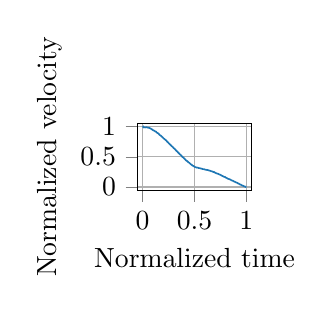
\begin{tikzpicture}

\definecolor{color0}{rgb}{0.12156862745098,0.466666666666667,0.705882352941177}

\begin{axis}[
xlabel={Normalized time},
ylabel={Normalized velocity},
xmin=-0.05, xmax=1.05,
ymin=-0.05, ymax=1.05,
width=\figurewidth,
height=\figureheight,
tick align=outside,
tick pos=left,
xmajorgrids,
x grid style={white!69.01960784313725!black},
ymajorgrids,
y grid style={white!69.01960784313725!black}
]
\addplot [semithick, color0, forget plot]
table {%
0 0.985915492957746
0.00680274027029168 1
0.0136054805405858 0.987323943661972
0.0204082208108775 0.988732394366197
0.0272110282176721 0.987323943661972
0.0340137684879662 0.991549295774648
0.0408165087582578 0.988732394366197
0.0476192490285519 0.987323943661972
0.0544219892988436 0.980281690140845
0.0612247295691377 0.98169014084507
0.0680274698394294 0.977464788732394
0.0748302101097235 0.970422535211268
0.0816329503800152 0.963380281690141
0.0884356906503093 0.957746478873239
0.095238430920601 0.947887323943662
0.102043319558936 0.940845070422535
0.115648800099522 0.929577464788732
0.122451540369816 0.919718309859155
0.129254280640107 0.916901408450704
0.136057020910402 0.902816901408451
0.142859761180693 0.894366197183099
0.149662501450987 0.890140845070422
0.156465241721279 0.87887323943662
0.163267981991573 0.863380281690141
0.170070722261865 0.856338028169014
0.176873462532159 0.849295774647887
0.183676202802451 0.835211267605634
0.190478943072745 0.828169014084507
0.197281683343036 0.814084507042254
0.20408442361333 0.802816901408451
0.210887163883622 0.794366197183099
0.217689904153916 0.784507042253521
0.224492644424208 0.774647887323944
0.231295384694502 0.763380281690141
0.238098124964794 0.746478873239437
0.244900865235088 0.740845070422535
0.251703672641882 0.725352112676056
0.258506412912174 0.714084507042253
0.265309153182468 0.704225352112676
0.27211189345276 0.691549295774648
0.278914633723054 0.67887323943662
0.285717373993346 0.670422535211267
0.292517965895596 0.659154929577465
0.299320706165891 0.64225352112676
0.306123446436182 0.638028169014084
0.312926119569973 0.623943661971831
0.319728926976768 0.609859154929577
0.326531667247062 0.598591549295775
0.333334407517354 0.588732394366197
0.340137147787648 0.574647887323944
0.34693988805794 0.563380281690141
0.353742628328234 0.552112676056338
0.360545368598525 0.538028169014084
0.367348108868819 0.530985915492958
0.374150849139111 0.519718309859155
0.380953589409405 0.501408450704225
0.394559069949991 0.485915492957746
0.401361810220283 0.470422535211268
0.408164550490577 0.461971830985915
0.414967290760868 0.446478873239437
0.421770031031163 0.436619718309859
0.428572771301454 0.430985915492958
0.435375511571748 0.419718309859155
0.44217825184204 0.408450704225352
0.448980992112334 0.401408450704225
0.455783732382626 0.390140845070422
0.46258647265292 0.37887323943662
0.469389212923212 0.373239436619718
0.476191953193506 0.361971830985915
0.482994693463797 0.352112676056338
0.489797433734091 0.349295774647887
0.496600174004383 0.340845070422535
0.503402914274677 0.332394366197183
0.517008394815263 0.325352112676056
0.523811135085555 0.32112676056338
0.530613875355849 0.322535211267606
0.53741661562614 0.315492957746479
0.551020149208187 0.312676056338028
0.557822889478481 0.308450704225352
0.564625629748773 0.305633802816901
0.571428370019067 0.302816901408451
0.578231110289358 0.297183098591549
0.591836590829944 0.295774647887324
0.598639331100238 0.290140845070422
0.612244811640824 0.285915492957746
0.619047551911116 0.283098591549296
0.62585029218141 0.28169014084507
0.632653032451702 0.280281690140845
0.639455772721996 0.274647887323944
0.653061253262581 0.267605633802817
0.659863993532876 0.261971830985915
0.673469474073461 0.257746478873239
0.680272214343753 0.249295774647887
0.687074954614047 0.250704225352113
0.693877694884339 0.242253521126761
0.700680435154633 0.236619718309859
0.707483175424925 0.229577464788732
0.714285915695219 0.225352112676056
0.72108865596551 0.22112676056338
0.727891396235804 0.219718309859155
0.734694136506096 0.212676056338028
0.74149687677639 0.205633802816901
0.748299617046682 0.204225352112676
0.755102357316976 0.195774647887324
0.761905097587268 0.190140845070423
0.768707837857562 0.184507042253521
0.775510578127853 0.177464788732394
0.782313318398147 0.171830985915493
0.789116058668439 0.167605633802817
0.795918798938733 0.164788732394366
0.802721539209025 0.154929577464789
0.809524279479319 0.150704225352113
0.816327019749611 0.142253521126761
0.823129760019905 0.136619718309859
0.829932500290196 0.133802816901408
0.836735240560491 0.129577464788732
0.843537980830782 0.125352112676056
0.850340721101076 0.11830985915493
0.857142454323848 0.109859154929577
0.863945194594142 0.107042253521127
0.870747934864434 0.102816901408451
0.877550675134728 0.0943661971830986
0.88435341540502 0.0915492957746479
0.891156155675314 0.0845070422535211
0.897958895945606 0.0774647887323944
0.9047616362159 0.0746478873239437
0.911564376486191 0.0690140845070423
0.918367116756485 0.0605633802816902
0.925169857026777 0.0577464788732394
0.931972597297071 0.0492957746478873
0.938775337567363 0.0422535211267606
0.945578077837657 0.0394366197183099
0.952380818107949 0.0323943661971831
0.959183558378243 0.0267605633802817
0.965986298648534 0.0225352112676056
0.972789038918828 0.0169014084507042
0.97959177918912 0.0112676056338028
0.986394519459414 0.00845070422535212
0.993197259729706 0.00140845070422538
1 0
};
\end{axis}

\end{tikzpicture}
	\end{figure}
\end{frame}

\begin{frame}{Measure performance}
	We can use the following performance measure:
	\begin{equation}
		J = \prod_{i=1}^n \int f(z,y_i) p(z) dz = \prod_{i=1}^n E[f(z,y_i)]
	\end{equation}
	\begin{itemize}
		\item $y_i$ denotes a normalized test curve (from real-life data).
		\item $z$ denotes generated (spline) parameters.
		\item $f(z,y_i)$ is a \emph{similarity function} that \emph{measures} how well the generated curve (using $z$) looks like the test curve $y_i$.
	\end{itemize}
	\pause
	Why such a strange function? Consider $f(z,y_i) = \delta(z-y_i)$ (assume we can subtract $y_i$ from $z$, $\delta(\cdot)$ represents Dirac function) and we get `just' cross-validation with likelihood:
	\begin{equation}
		J = \prod_{i=1}^n p(y_i)
	\end{equation}
\end{frame}


\begin{frame}{Measure performance}
	We can estimate $J$ using a Monte Carlo approach with large $N$:
	\begin{equation}
		J \approx \prod_{i=1}^n \sum_{j=1}^N f(z_j, y_i), \quad z_j \sim p(Z)
	\end{equation}
	How to define $f(z,y)$? \pause One approach involves the product integral ($g_z(t)$ is the spline generated with parameters $z$):
	\begin{equation}
		f(z, y) = \prod_{t=0}^1 \left( \frac{1}{\sqrt{2\pi\sigma^2}} \exp \left\{ -\frac{\left(y(t) - g_z(t)\right)^2}{2\sigma^2} \right\} \right)^{dt}
	\end{equation}
	The intuition behind this function is that the generated curve should match everywhere, not at only one time instant (then a normal integral would suffice).
\end{frame}

\begin{frame}{Simple case example}
	\begin{figure}
		\centering
		% This file was created by matplotlib2tikz v0.6.14.
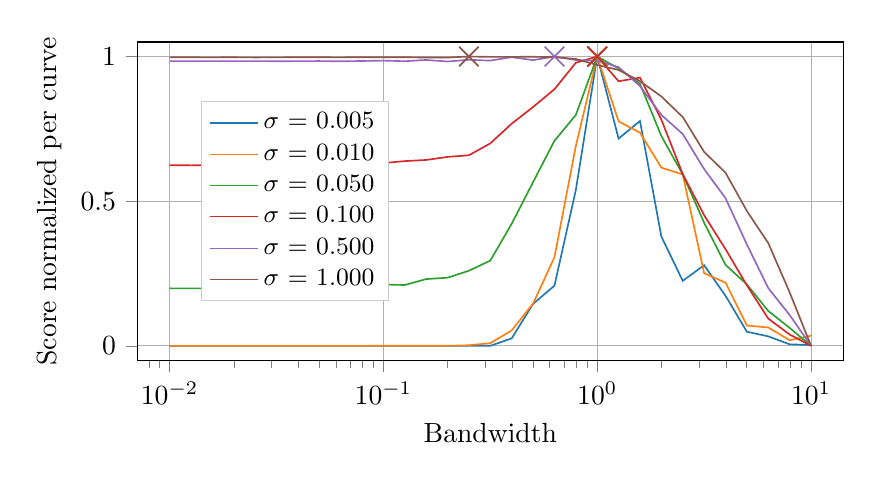
\begin{tikzpicture}

\definecolor{color4}{rgb}{0.580392156862745,0.403921568627451,0.741176470588235}
\definecolor{color5}{rgb}{0.549019607843137,0.337254901960784,0.294117647058824}
\definecolor{color0}{rgb}{0.12156862745098,0.466666666666667,0.705882352941177}
\definecolor{color1}{rgb}{1,0.498039215686275,0.0549019607843137}
\definecolor{color3}{rgb}{0.83921568627451,0.152941176470588,0.156862745098039}
\definecolor{color2}{rgb}{0.172549019607843,0.627450980392157,0.172549019607843}

\begin{axis}[
xlabel={Bandwidth},
ylabel={Score normalized per curve},
xmin=0.00707945784384139, xmax=14.1253754462275,
ymin=-0.05, ymax=1.05,
xmode=log,
width=300pt,
height=160pt,
tick align=outside,
tick pos=left,
xmajorgrids,
x grid style={white!69.019607843137251!black},
ymajorgrids,
y grid style={white!69.019607843137251!black},
legend style={at={(0.09,0.5)}, anchor=west, draw=white!80.0!black},
legend entries={{$\sigma$ = 0.005},{$\sigma$ = 0.010},{$\sigma$ = 0.050},{$\sigma$ = 0.100},{$\sigma$ = 0.500},{$\sigma$ = 1.000}},
legend cell align={left}
]
\addlegendimage{no markers, color0}
\addlegendimage{no markers, color1}
\addlegendimage{no markers, color2}
\addlegendimage{no markers, color3}
\addlegendimage{no markers, color4}
\addlegendimage{no markers, color5}
\addplot [semithick, color0]
table {%
0.01 0
0.0125892541179417 3.45772981158938e-14
0.0158489319246111 4.63409779464337e-14
0.0199526231496888 1.44873072719401e-13
0.0251188643150958 1.99156297046487e-13
0.0316227766016838 4.40127970898054e-13
0.0398107170553497 7.59549531744384e-13
0.0501187233627272 1.56646629536674e-12
0.0630957344480193 3.82695176499514e-12
0.0794328234724281 1.14859712910995e-11
0.1 2.56090937937578e-11
0.125892541179417 2.22997251700408e-10
0.158489319246111 3.43509788493226e-09
0.199526231496888 1.52983568182557e-07
0.251188643150958 1.36551103668467e-07
0.316227766016838 3.25863863615824e-05
0.398107170553497 0.0256907561615501
0.501187233627272 0.144926086169419
0.630957344480193 0.207884760614761
0.794328234724282 0.538347731930234
1 1
1.25892541179417 0.716376085623372
1.58489319246111 0.777083672870848
1.99526231496888 0.377836725769632
2.51188643150958 0.224589443615349
3.16227766016838 0.278635237242103
3.98107170553497 0.173097406030044
5.01187233627272 0.0486957961204249
6.30957344480194 0.0327342432696328
7.94328234724282 0.00526458447070756
10 0.00270552142319118
};
\addplot [semithick, color0, mark=x, mark size=5, mark options={solid}, only marks, forget plot]
table {%
1 1
};
\addplot [semithick, color1]
table {%
0.01 0
0.0125892541179417 7.10094370372152e-08
0.0158489319246111 5.21561087913403e-08
0.0199526231496888 9.72967979089316e-08
0.0251188643150958 2.56250082524174e-07
0.0316227766016838 4.10158728766311e-07
0.0398107170553497 5.48312122562301e-07
0.0501187233627272 7.70561536838568e-07
0.0630957344480193 1.96199378903389e-06
0.0794328234724281 3.12799407949813e-06
0.1 5.74753542675034e-06
0.125892541179417 1.24382585605373e-05
0.158489319246111 3.04648190894159e-05
0.199526231496888 7.94417937545628e-05
0.251188643150958 0.00204134788492363
0.316227766016838 0.0090604670329023
0.398107170553497 0.0533258588760914
0.501187233627272 0.14573696048373
0.630957344480193 0.306068954536085
0.794328234724282 0.690767402705991
1 1
1.25892541179417 0.775862831301648
1.58489319246111 0.736674913239406
1.99526231496888 0.615926696224473
2.51188643150958 0.592108721846232
3.16227766016838 0.251265324442236
3.98107170553497 0.218485399857015
5.01187233627272 0.0701633305809969
6.30957344480194 0.0633794210688501
7.94328234724282 0.0193606222179061
10 0.035133756096109
};
\addplot [semithick, color1, mark=x, mark size=5, mark options={solid}, only marks, forget plot]
table {%
1 1
};
\addplot [semithick, color2]
table {%
0.01 0.198757419559841
0.0125892541179417 0.198552510341383
0.0158489319246111 0.198693826746533
0.0199526231496888 0.199139866697188
0.0251188643150958 0.198254555626781
0.0316227766016838 0.199287307649665
0.0398107170553497 0.200648938029905
0.0501187233627272 0.199746164436195
0.0630957344480193 0.201893634744242
0.0794328234724281 0.206456861730369
0.1 0.212045558495366
0.125892541179417 0.210191370961082
0.158489319246111 0.230632422854846
0.199526231496888 0.23553546528526
0.251188643150958 0.259538385651183
0.316227766016838 0.294635283995112
0.398107170553497 0.421552711191689
0.501187233627272 0.565645559303058
0.630957344480193 0.708657486588031
0.794328234724282 0.797725135295843
1 1
1.25892541179417 0.958626465917236
1.58489319246111 0.90575084206707
1.99526231496888 0.725044483490716
2.51188643150958 0.592641927876395
3.16227766016838 0.425581094025592
3.98107170553497 0.27998694504141
5.01187233627272 0.212154875840917
6.30957344480194 0.12041808077881
7.94328234724282 0.0619783792470194
10 0
};
\addplot [semithick, color2, mark=x, mark size=5, mark options={solid}, only marks, forget plot]
table {%
1 1
};
\addplot [semithick, color3]
table {%
0.01 0.624092994824543
0.0125892541179417 0.623873617845941
0.0158489319246111 0.623990952475475
0.0199526231496888 0.623697730680669
0.0251188643150958 0.623996506285411
0.0316227766016838 0.625393842293304
0.0398107170553497 0.626951385459326
0.0501187233627272 0.625744487299428
0.0630957344480193 0.627412764412564
0.0794328234724281 0.62823927670166
0.1 0.63175700444986
0.125892541179417 0.638445388804656
0.158489319246111 0.6424613466771
0.199526231496888 0.652926639818827
0.251188643150958 0.658713839636203
0.316227766016838 0.699662612793462
0.398107170553497 0.767810112169875
0.501187233627272 0.825431142800018
0.630957344480193 0.886838305984548
0.794328234724282 0.978356964920904
1 1
1.25892541179417 0.91450175817467
1.58489319246111 0.9269847958991
1.99526231496888 0.781881520251036
2.51188643150958 0.593585398304157
3.16227766016838 0.451569335925889
3.98107170553497 0.334105470092901
5.01187233627272 0.209022117578504
6.30957344480194 0.0940190285121043
7.94328234724282 0.0390820881087768
10 0
};
\addplot [semithick, color3, mark=x, mark size=5, mark options={solid}, only marks, forget plot]
table {%
1 1
};
\addplot [semithick, color4]
table {%
0.01 0.984063129951187
0.0125892541179417 0.984149835771952
0.0158489319246111 0.984161924202251
0.0199526231496888 0.984177669399439
0.0251188643150958 0.984157866042631
0.0316227766016838 0.983790935809609
0.0398107170553497 0.983968226848383
0.0501187233627272 0.984253289702716
0.0630957344480193 0.98343538276351
0.0794328234724281 0.984497635223848
0.1 0.98584551944141
0.125892541179417 0.983725320974544
0.158489319246111 0.988067516838301
0.199526231496888 0.982757216856586
0.251188643150958 0.98864760086515
0.316227766016838 0.985840879317049
0.398107170553497 0.997690836597155
0.501187233627272 0.987475223195824
0.630957344480193 1
0.794328234724282 0.987926512919797
1 0.985664512446548
1.25892541179417 0.963041581683622
1.58489319246111 0.898017976488242
1.99526231496888 0.798005872180785
2.51188643150958 0.732225348764683
3.16227766016838 0.610972235472318
3.98107170553497 0.510494007379659
5.01187233627272 0.350211212569661
6.30957344480194 0.199386030727152
7.94328234724282 0.106510419151888
10 0
};
\addplot [semithick, color4, mark=x, mark size=5, mark options={solid}, only marks, forget plot]
table {%
0.630957344480193 1
};
\addplot [semithick, color5]
table {%
0.01 0.9971678051717
0.0125892541179417 0.99721927057446
0.0158489319246111 0.997110599591715
0.0199526231496888 0.997261266444183
0.0251188643150958 0.996819120965199
0.0316227766016838 0.997044632138514
0.0398107170553497 0.997392145410018
0.0501187233627272 0.997335026106395
0.0630957344480193 0.997029725064975
0.0794328234724281 0.997703380669255
0.1 0.997226689226201
0.125892541179417 0.997492818910047
0.158489319246111 0.99644398048946
0.199526231496888 0.996471764792833
0.251188643150958 1
0.316227766016838 0.9987252730855
0.398107170553497 0.998839106850672
0.501187233627272 0.999011636397847
0.630957344480193 0.997870780982989
0.794328234724282 0.991440084388769
1 0.970753111142074
1.25892541179417 0.95337067592214
1.58489319246111 0.914724295656003
1.99526231496888 0.861942997526599
2.51188643150958 0.790788352001693
3.16227766016838 0.670312910345563
3.98107170553497 0.598358912165044
5.01187233627272 0.466091835174457
6.30957344480194 0.355012316291236
7.94328234724282 0.184757937911024
10 0
};
\addplot [semithick, color5, mark=x, mark size=5, mark options={solid}, only marks, forget plot]
table {%
0.251188643150958 1
};
\end{axis}

\end{tikzpicture}
		\vspace{-0.5em}
		\caption{Normalized score versus the bandwidth for a simple case study with different values for $\sigma$.}
	\end{figure}
\end{frame}

\begin{frame}{Future work}
	\begin{columns}
		\begin{column}{0.46\textwidth}
			Use Singular Value Decomposition (SVD) to
			\begin{itemize}
				\item lower the number of parameters;
				\item effectively change kernel.
			\end{itemize}
		\end{column}
		\begin{column}{0.55\textwidth}
			\begin{figure}
				\vspace{-2em}
				% This file was created by matplotlib2tikz v0.6.14.
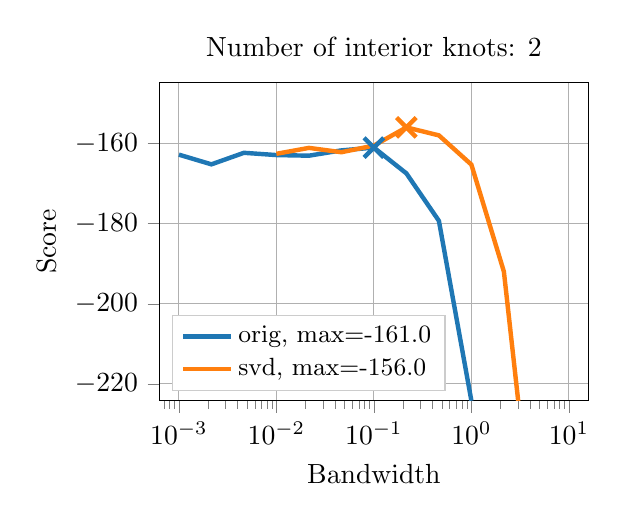
\begin{tikzpicture}

\definecolor{color1}{rgb}{1,0.498039215686275,0.0549019607843137}
\definecolor{color0}{rgb}{0.12156862745098,0.466666666666667,0.705882352941177}

\begin{axis}[
title={Number of interior knots: 2},
xlabel={Bandwidth},
ylabel={Score},
xmin=0.000630957344480194, xmax=15.8489319246111,
ymin=-224.189971573679, ymax=-144.782638312349,
xmode=log,
width=200pt,
height=160pt,
tick align=outside,
tick pos=left,
xmajorgrids,
x grid style={white!69.019607843137251!black},
ymajorgrids,
y grid style={white!69.019607843137251!black},
legend entries={{orig, max=-161.0},{svd, max=-156.0}},
legend cell align={left},
legend style={at={(0.03,0.03)}, anchor=south west, draw=white!80.0!black}
]
\addlegendimage{ultra thick, no markers, color0}
\addlegendimage{ultra thick, no markers, color1}
\addplot [ultra thick, color0]
table {%
0.001 -162.788480806602
0.00215443469003188 -165.20908464927
0.00464158883361278 -162.328839700755
0.01 -162.894086028145
0.0215443469003188 -163.048235338592
0.0464158883361278 -161.725459550645
0.1 -161.028188209683
0.215443469003188 -167.464121758257
0.464158883361278 -179.302600897359
1 -224.189971573679
};
\addplot [ultra thick, color0, mark=x, mark size=5, mark options={solid}, only marks, forget plot]
table {%
0.1 -161.028188209683
};
\addplot [ultra thick, color1]
table {%
0.01 -162.579092135606
0.0215443469003188 -161.101296218654
0.0464158883361278 -162.181949646304
0.1 -160.5240500964
0.215443469003188 -155.983015894602
0.464158883361278 -157.977551112033
1 -165.279039388593
2.15443469003188 -191.966290817474
4.64158883361278 -265.208066719389
10 -379.990567539667
};
\addplot [ultra thick, color1, mark=x, mark size=5, mark options={solid}, only marks, forget plot]
table {%
0.215443469003188 -155.983015894602
};
\end{axis}

\end{tikzpicture}
			\end{figure}
		\end{column}
	\end{columns}
\end{frame}

\begin{frame}{Future work}
	Use of copulas \cite{Schmidt2007, scaillet2007estimationcopulas, aas2009paircopula}
	\begin{itemize}
		\item Copulas are well-known for being good in estimating the tails of PDFs.
		\item Work in progress...
		\item Theory is promising, but no good working example so far.
	\end{itemize}
\end{frame}

\section{Conclusion}
\stepcounter{subsection}
\begin{frame}{Conclusion}
	\begin{itemize}
		\item Parametrization and PDF estimation are crucial for the scenario generation.
		\item We need a good measure to quantify how good the parametrization and PDF estimation are.
		\item Lots of future work...
	\end{itemize}
\end{frame}

\section{References}
\stepcounter{subsection}
\begin{frame}{References}
\end{frame}

\begin{frame}[allowframebreaks]
	%\frametitle{References}  % This gives an error...
	\scriptsize{\bibliographystyle{ieeetran}}
	\bibliography{../bib}
\end{frame}

\end{document}